\chapter{Adding relationships in Gaussian Process}
\label{chapAddingEquationsInGP}

\section{Multi-output Gaussian Process}\label{sec:mogp}

\noindent Given a dataset for multiple outputs \(\{(x_{i}, y_{i})\}\) for \(i \in [1; D]\) we define the joint output vector \(Y = [y_{1}; y_{2}; y_{3}; \ldots; y_{D}]\) such that all the output values are stacked one after the other. Similarly, we define the joint input matrix as \(X = [x_{1}; x_{2}; x_{3}; \ldots; x_{D}]\). For the sake of simplicity, suppose we measure two outputs  \(y_{1}\) and \(y_{2}\) with some error, while the true physical process is defined by latent variables \(f_{1}\) and \(f_{2}\) equation \ref{eq:physicalRelation}. The operator \(g(.)\) can be a known physical equation or a computer code between the outputs, it basically represents a transformation from one output to another. 

\subsection{Related Work}\label{subsec:MOGPrelatedWork}
Earlier work developing such joint-covariance functions \cite{bonilla_multi-task_2008} have focused on  building different outputs as a combination of a set of latent functions. GP priors are placed independently over all the latent functions thereby inducing a correlated covariance function. More recently it has been shown that convolution processes \cite{journals/jmlr/AlvarezLL09} ,   \cite{Boyle05dependentgaussian} can be used to develop joint-covariance functions for differential equations. In a convolution process framework output functions are generated by convolving several latent functions with a smoothing kernel function. In the current paper we assume one output function to be independent and evaluate the remaining auto- and cross-covariance functions exactly if the physical relation between them is linear \cite{NIPSDerivativeGP} or use approximate joint-covariance for non-linear physics-based relationships between the outputs \cite{Constantinescu2013}.

\subsection{Multi-output Joint-covariance kernels}\label{sub:MOGPs}
A GP prior in such a setting with 2 output variables is expressed in equation \ref{eq:mogpJointPrior}.  

   \begin{equation}\label{eq:mogpJointPrior}
   \begin{bmatrix}
   f_{1}\\
   f_{2}
   
   \end{bmatrix} \sim GP\begin{bmatrix}
   \begin{pmatrix}
   0\\ 
   0
   \end{pmatrix} ,& 
   \begin{pmatrix}
   K_{11}  & K_{12}\\ K_{21}
    & K_{22}
   \end{pmatrix}
   \end{bmatrix}
   \end{equation}
   
   
   \(K_{12}\) and \(K_{21}\) are cross-covariances between the two inputs \(x_{1}\) and \(x_{2}\). \(K_{22}\) is the auto-covariance function of independent output, while \(K_{11}\) is the auto-covariance of the dependent output variable. The full covariance matrix \(K_{XX}\) is also called the joint-covariance. While, the joint error matrix will be denoted by \(\Sigma\);
         \begin{equation}\label{eq:sigmaToError}
         \Sigma = 
          \begin{bmatrix}
          \sigma _{n1}^{2} & 0 \\ 
          0 & \sigma _{n2}^{2}
          \end{bmatrix} 
         \end{equation}
         
      Where, \(\epsilon_{n1}\) and \(\epsilon_{n2}\) are measurement error sampled from a white noise gaussian \(\mathcal{N}(0, \sigma_{n1})\) and \(\mathcal{N}(0, \sigma_{n2})\). 
      
    For a linear operator \(g(.)\) the joint-covariance matrix can be derived analytically \cite{Stein1999Springer}, due to the affine property of Gaussian's equation \ref{eq:exactJointCovariance}. 
   
    \begin{equation}\label{eq:exactJointCovariance}
    \begin{bmatrix}
    f_{1}\\
    f_{2}
      
    \end{bmatrix} \sim GP\begin{bmatrix}
    \begin{pmatrix}
    0\\ 
    0
    \end{pmatrix} ,& 
    \begin{pmatrix}
    g(g(K_{22}, x_{2}), x_{1}) & g(K_{22}, x_{1})\\ g(K_{22}, x_{2}) & K_{22}
    \end{pmatrix} 
    \end{bmatrix}
    \end{equation}
      
   Using the known relation between outputs we have successfully correlated two GP priors from equation \ref{eq:physicalRelation}. This effectively means that when we randomly draw a function \(f_{2}\) it will result in a correlated draw of \(f_{1}\) such that the two draws satisfy the equation \ref{eq:physicalRelation}. We have effectively represented the covariance function \(K_{11}\) in terms of the hyperparameters of covariance function \(K_{22}\) using the known relation between outputs.

\begin{figure}[!t]
  \centering
  \subfigure[Joint draws between \(f_{1}\) \(red\) and \(f_{2}\) \(blue\) such that \(f_{1} = \frac{\partial f_{2}}{\partial x}\).]
  {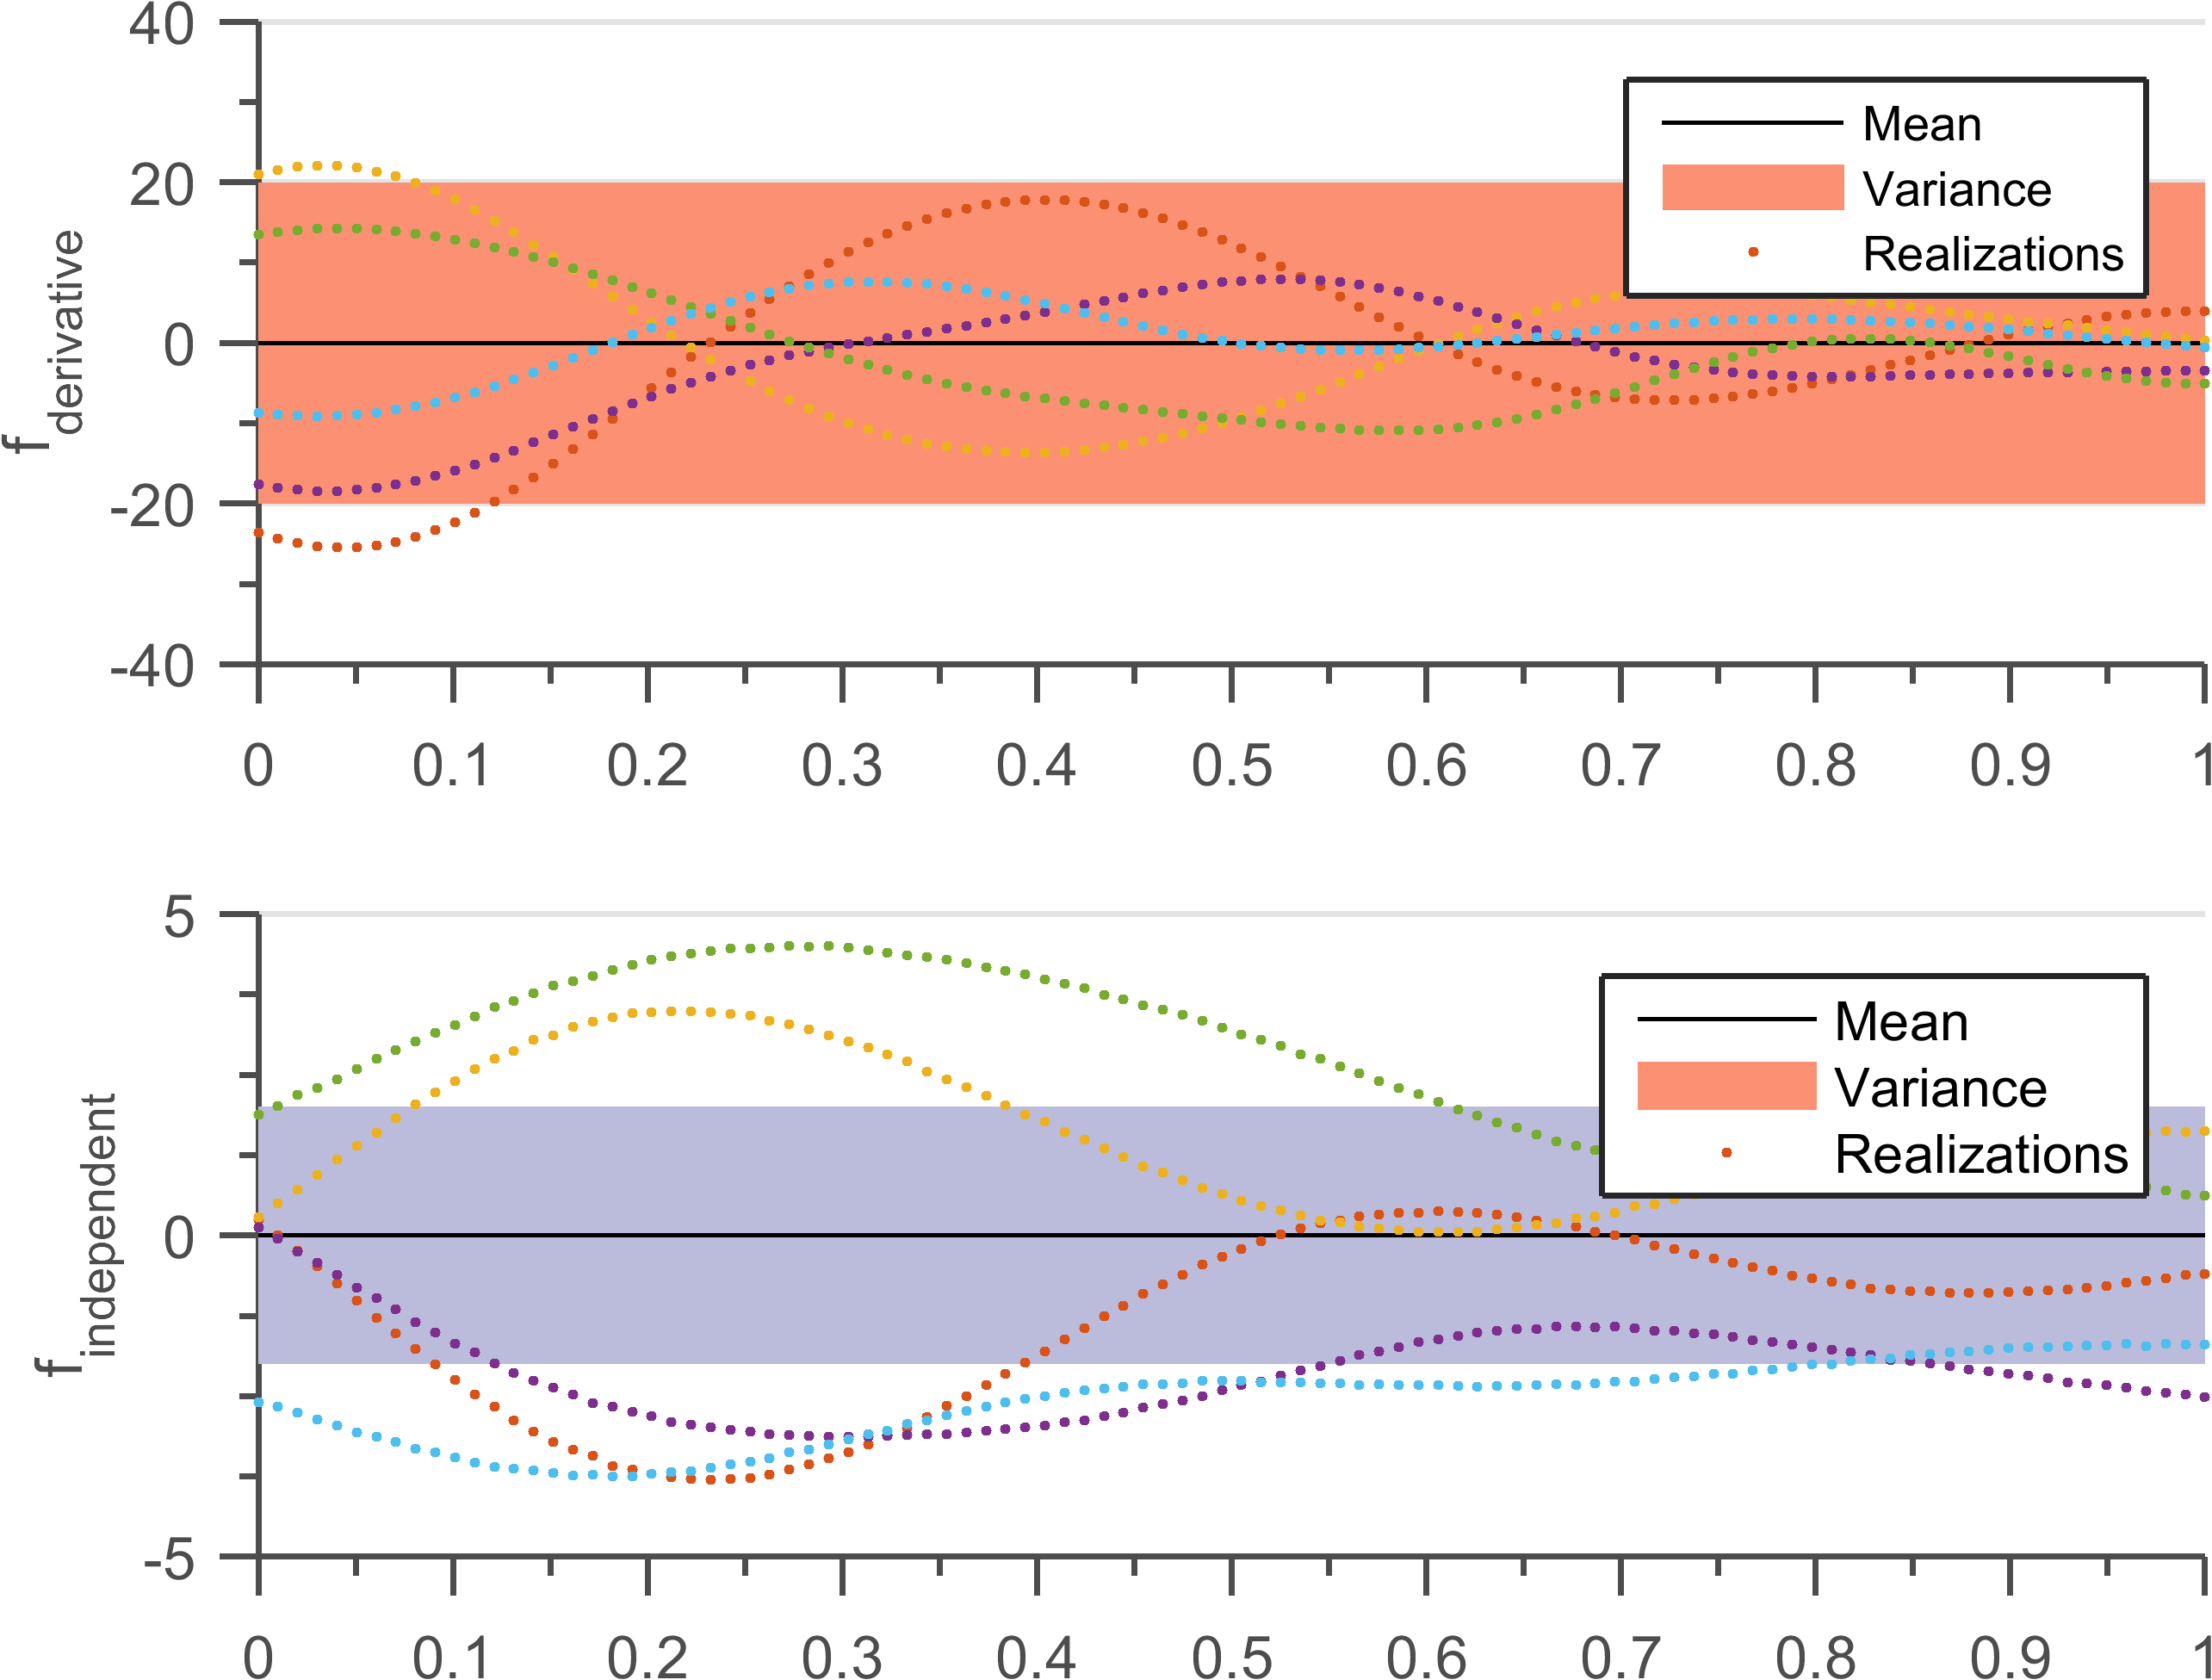
\includegraphics[width=0.485\textwidth]{images/drawsPriorDifferentialRelationship}\label{subfig:drawsPriorDifferentialRelationship}}\quad
  \subfigure[Joint draws between \(f_{1}\) \(red\) and \(f_{2}\) \(blue\) such that \(f_{1} = \int f_{2}\).]
  {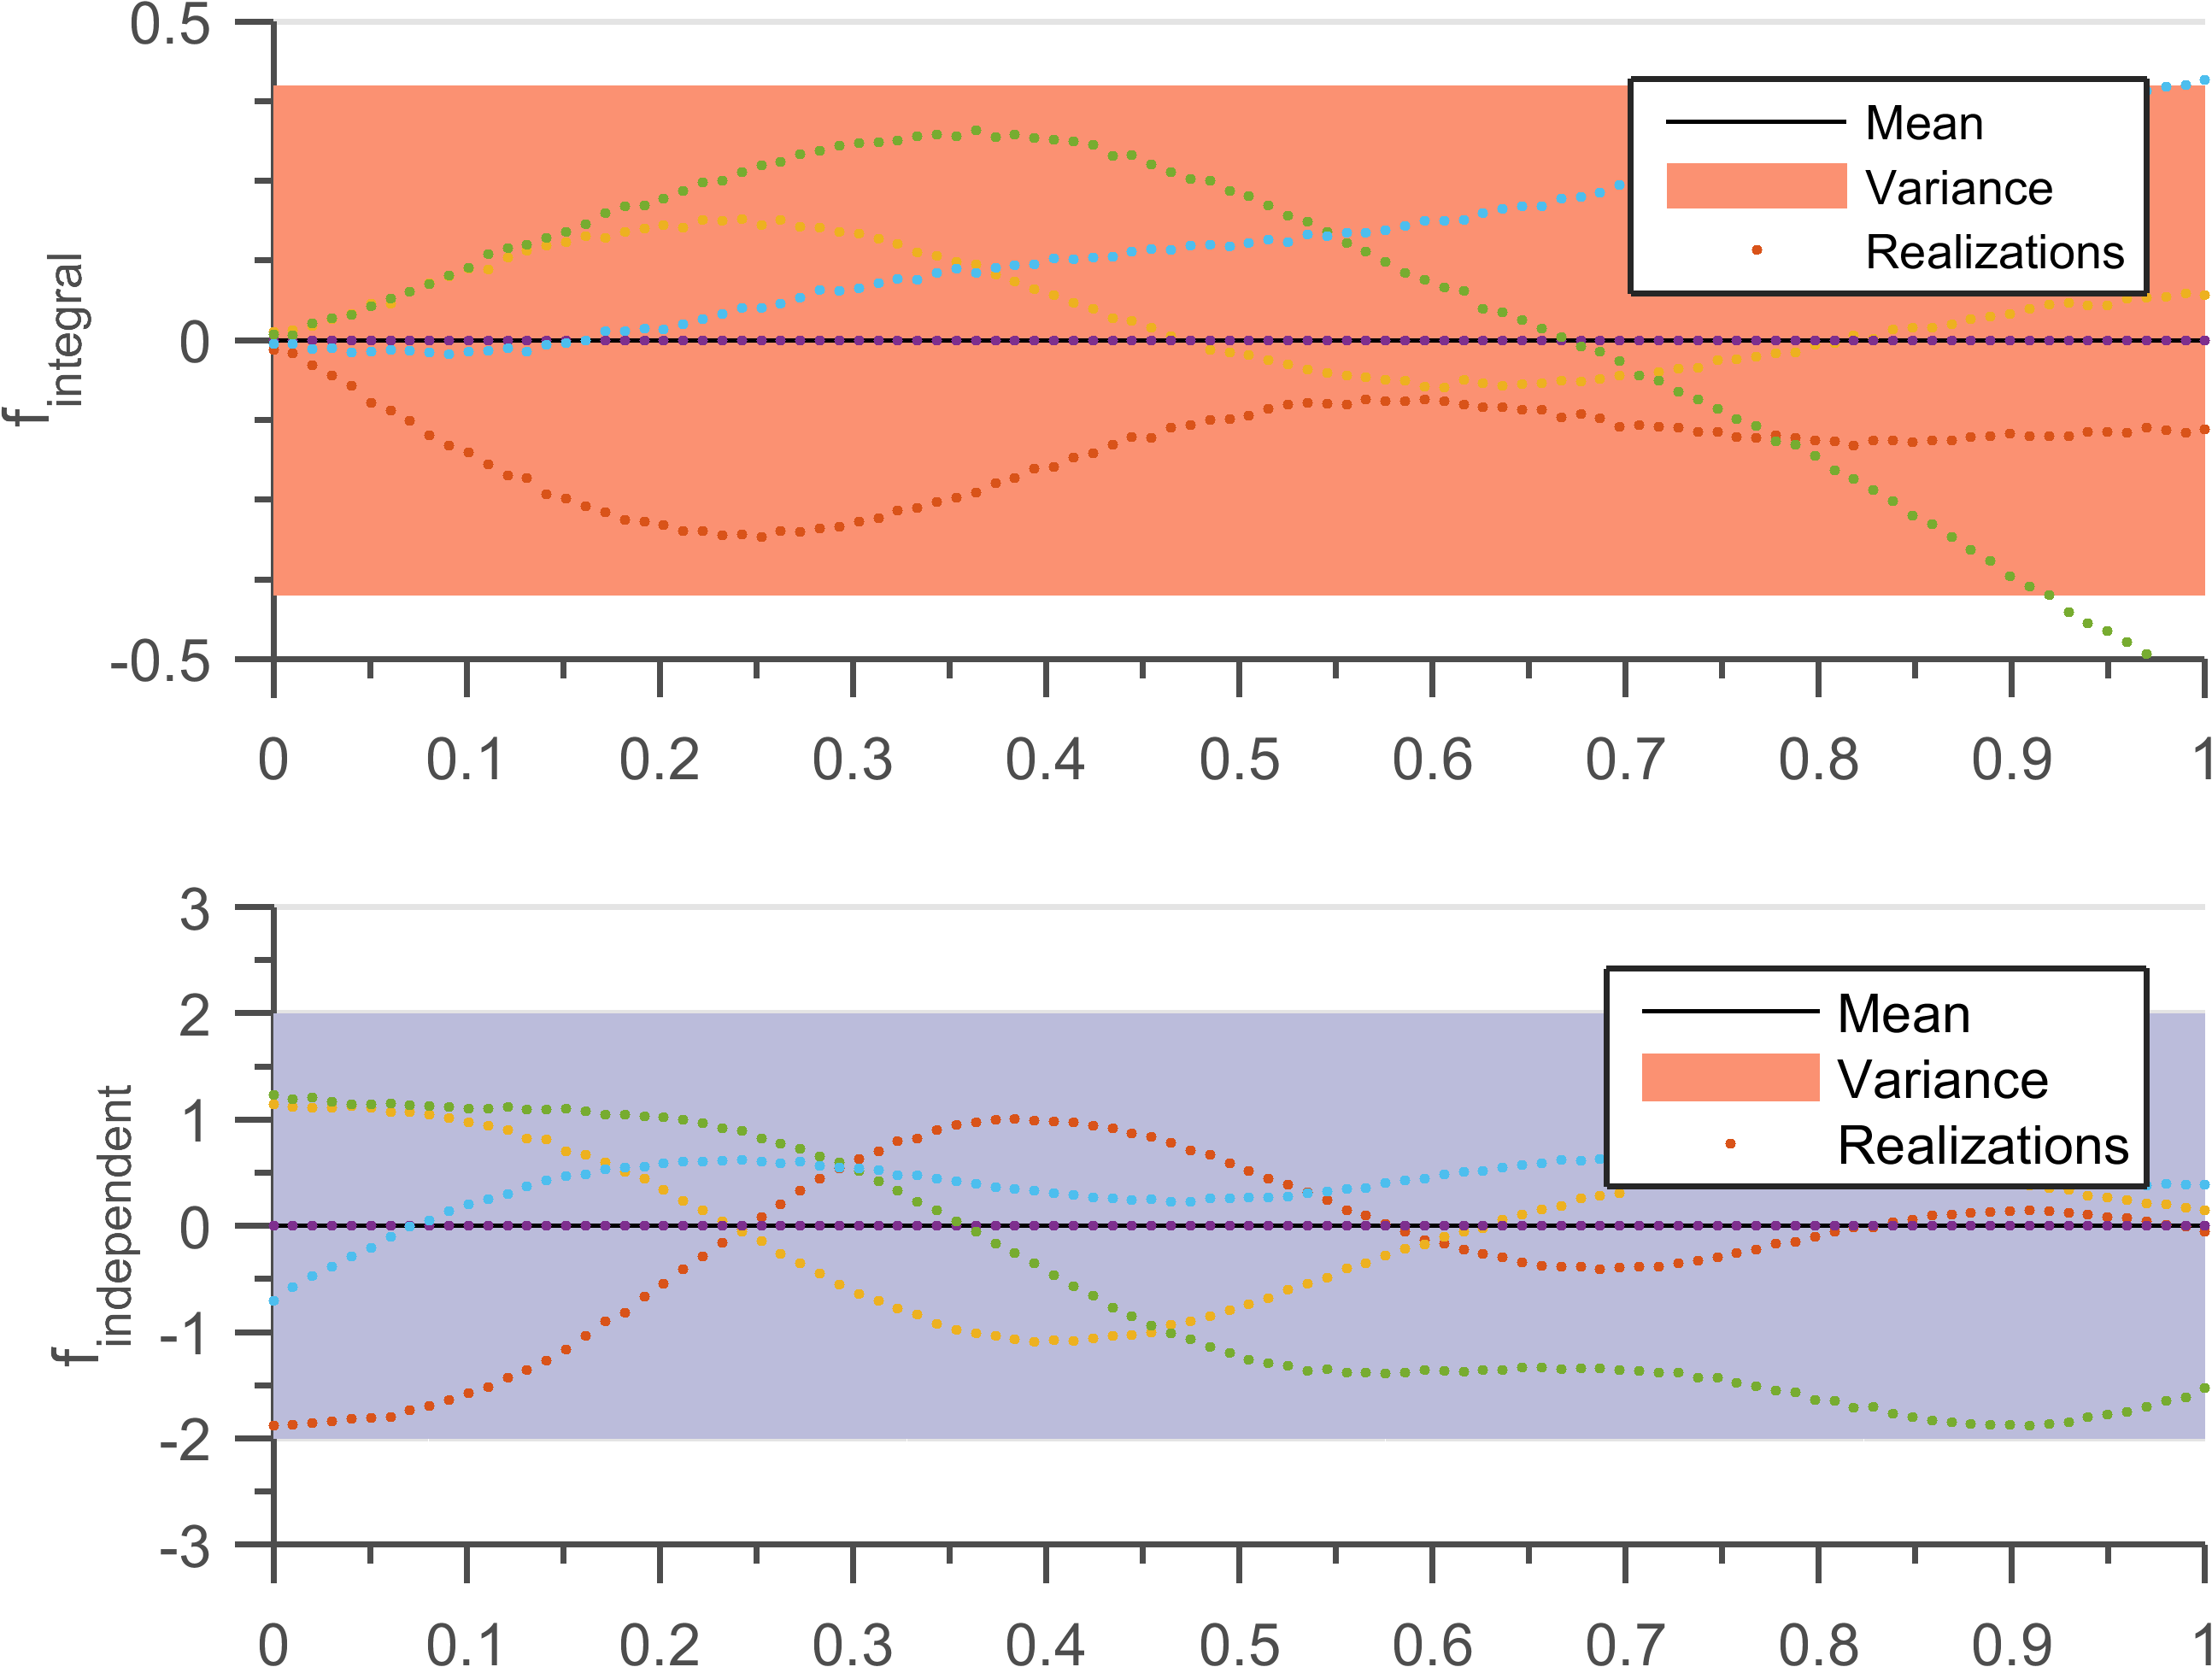
\includegraphics[width=0.485\textwidth]{images/drawsPriorIntegralRelationship}\label{subfig:drawsPriorIntegralRelationship}}
  \caption{Multi-Output Gaussian Process Random Draws}
\end{figure}

Without loss of generality we can assume that the independent output \(f_{2}\) belongs to a family of functions defined by a Squared Exponential kernel. The joint-covariance between \(f_{1}\) and \(f_{2}\), means that a random draw of independent function \(f_{2}\) will result in a correlated draw of the function \(f_{1}\). The fig: \ref{subfig:drawsPriorDifferentialRelationship} shows random draws coming from a differential relationship between \(f_{1}\) (red) and \(f_{2}\) (blue) such that \(f_{1} = \frac{\partial f_{2}}{\partial x}\). We can see that the top figure is derivative of the bottom one since \(f_{derivative}\) goes to zero where \(f_{independent}\) goes to maxima or minima. Similarly, the fig: \ref{subfig:drawsPriorIntegralRelationship} shows random draws coming from an integral relationship between \(f_{1}\) (red) and \(f_{2}\) (blue) such that \(f_{1} = \int f_{2}\). We can see that the top figure is integral of the bottom one since \(f_{independent}\) goes to zero where \(f_{integral}\) goes to maxima or minima. 

\subsection{GP Regression Using Joint-Covariance }\label{sub:GPUsingJointKernel}


We start with defining a zero-mean prior for our observations and make predictions for \(y_{1}\left ( x_{*} \right ) = y_{*1}\) and \(y_{2}\left ( x_{*} \right ) = y_{*2}\). The corresponding prior according to equation \ref{eq:mogpJointPrior} and \ref{eq:sigmaToError} will be:
 
 \begin{equation}\label{eq:MOGPPrior}
 \begin{bmatrix}
   Y(X))\\ 
   Y(X_{*}))
   \end{bmatrix} = GP\begin{bmatrix}
   \begin{bmatrix}
   0\\ 
   0
   \end{bmatrix}, 
   & 
   \begin{bmatrix}
   K_{XX} + \Sigma & K_{XX_{*}}\\ 
   K_{X_{*}X} & K_{X_{*}X_{*}} + \Sigma
   \end{bmatrix} 

   \end{bmatrix} 
 \end{equation}

  
  The posterior distribution is then given as a normal distribution with expectation and covariance matrix given by \cite{Rasmussen2005}
  \begin{equation}\label{eq:predictiveMOMean}
  m(y_{*}) = K_{X_{*}X}\left ( K_{XX} \right )^{-1}Y
  \end{equation}
  \begin{equation}\label{eq:predictiveMOCovariance}
  Cov(y_{*}) = K_{X_{*}X_{*}} - K_{X_{*}X}\left ( K_{XX} \right )^{-1}K_{XX_{*}}
  \end{equation}
  
  Here, the elements \(K_{XX}\), \(K_{X_{*}X}\) and \(K_{X_{*}X_{*}}\) are block covariances derived from equations \ref{eq:exactJointCovariance}. Due to the bayesian setting we have basically eliminated all the functions that do not pass through the points defined by the observed data.
  
  The joint-covariance matrix depends on several hyperparameters \(\theta\). They define a basic shape of the GP prior. To end up with good predictions it is important to start with a good GP prior. We minimize the negative log-marginal likelihood to find a set of good hyperparameters. This leads to an optimization problem where the objective function is given by equation \ref{eq:exactMONLML} 
  
  \begin{equation}\label{eq:exactMONLML}
\log(\mathbb{P}(y\mid X, \theta )) = \log[GP(Y| 0, K_{XX} + \Sigma )]
  \end{equation}
  
  With its gradient given by equation \ref{eq:gradientNLML}
  \begin{multline}\label{eq:gradientNLML}
 \frac{\partial }{\partial \theta}\log(\mathbb{P}(y\mid X, \theta )) = 
\frac{1}{2}Y^{T}K_{XX}^{-1}\frac{\partial K_{XX}}{\partial \theta}K_{XX}^{-1}Y \\
- \frac{1}{2}tr(K_{XX}^{-1}\frac{\partial K_{XX}}{\partial \theta})  
  \end{multline}

\begin{figure}[!t]
  \centering
  \subfigure[Joint draws between \(f_{1}\) \(red\) and \(f_{2}\) \(blue\) such that \(f_{1} = \frac{\partial f_{2}}{\partial x}\). The posterior is conditioned such that \(f_{1} = 5; x = 0\) and \(f_{2} = 0; x = 0\). The draws from the posterior follow the relationship between outputs and also the conditioning.]
  {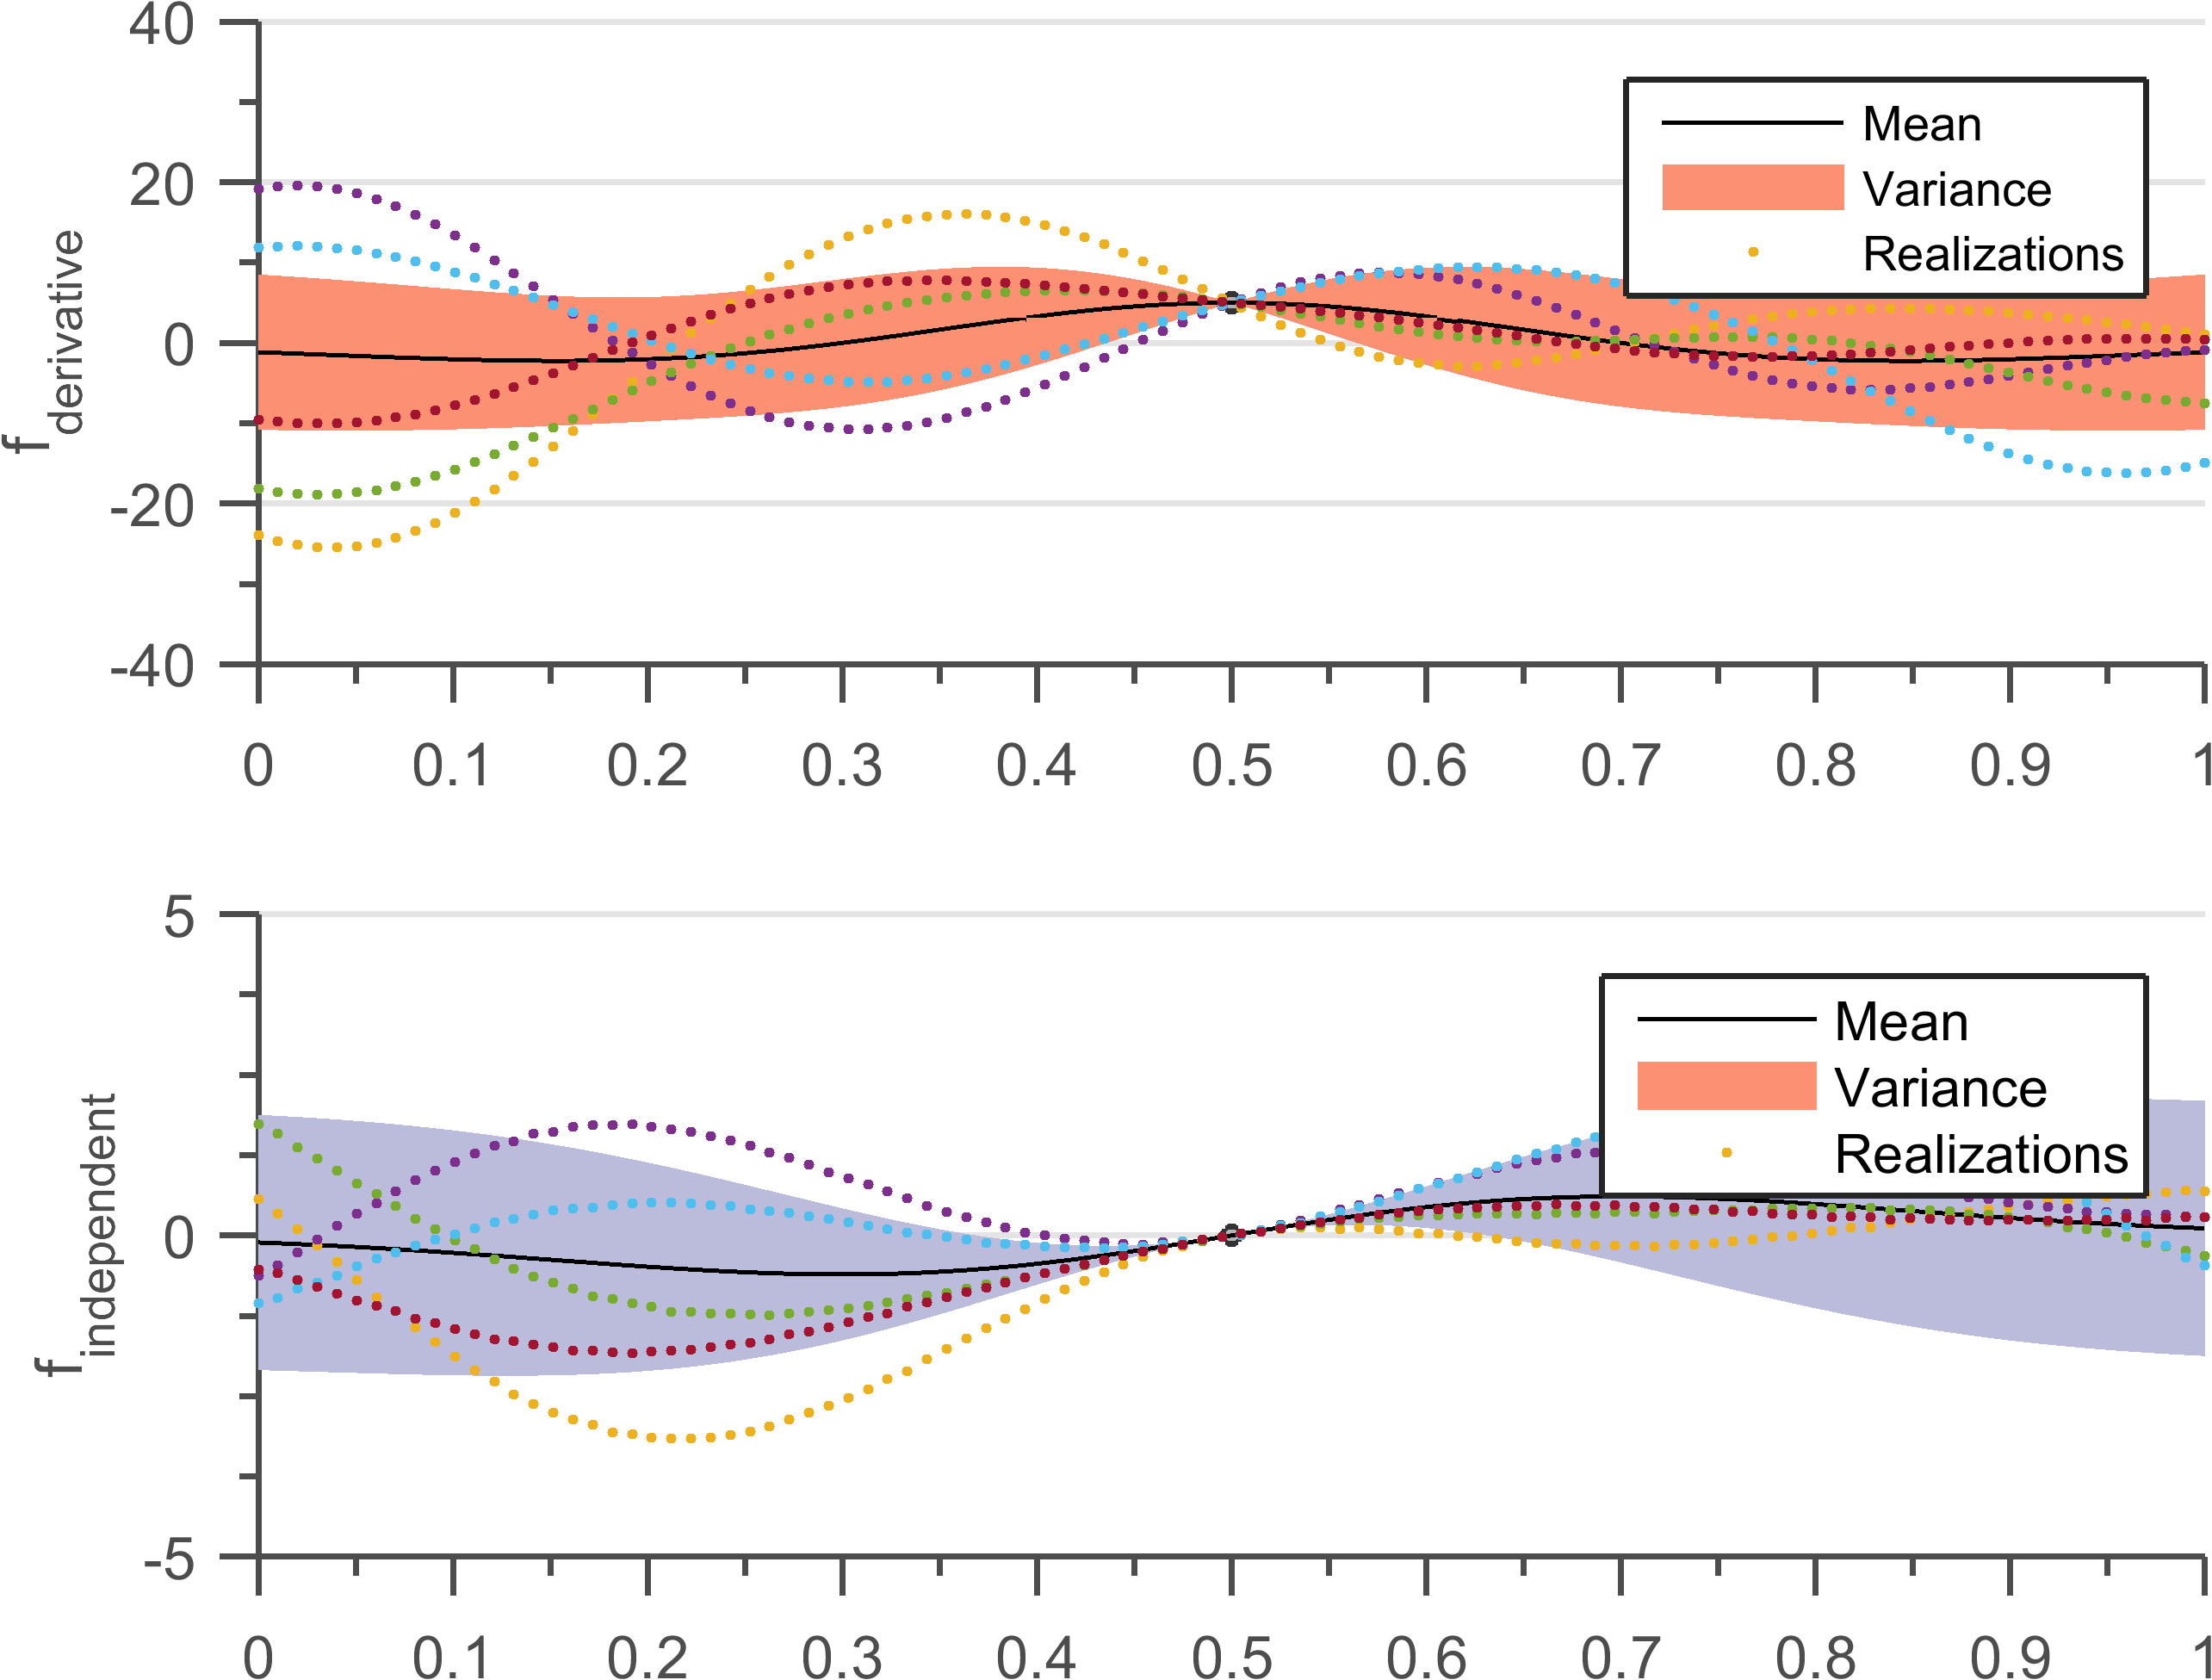
\includegraphics[width=0.485\textwidth]{images/drawsDifferentialRelationship}\label{subfig:drawsDifferentialRelationship}}\quad
  \subfigure[Joint draws between \(f_{1}\) \(red\) and \(f_{2}\) \(blue\) such that \(f_{1} = \int f_{2}\). The posterior is conditioned such that \(f_{1} = 0; x = 0\) and \(f_{1} = 0; x = 1\). The draws from the posterior follow the relationship between outputs and also the conditioning.]
  {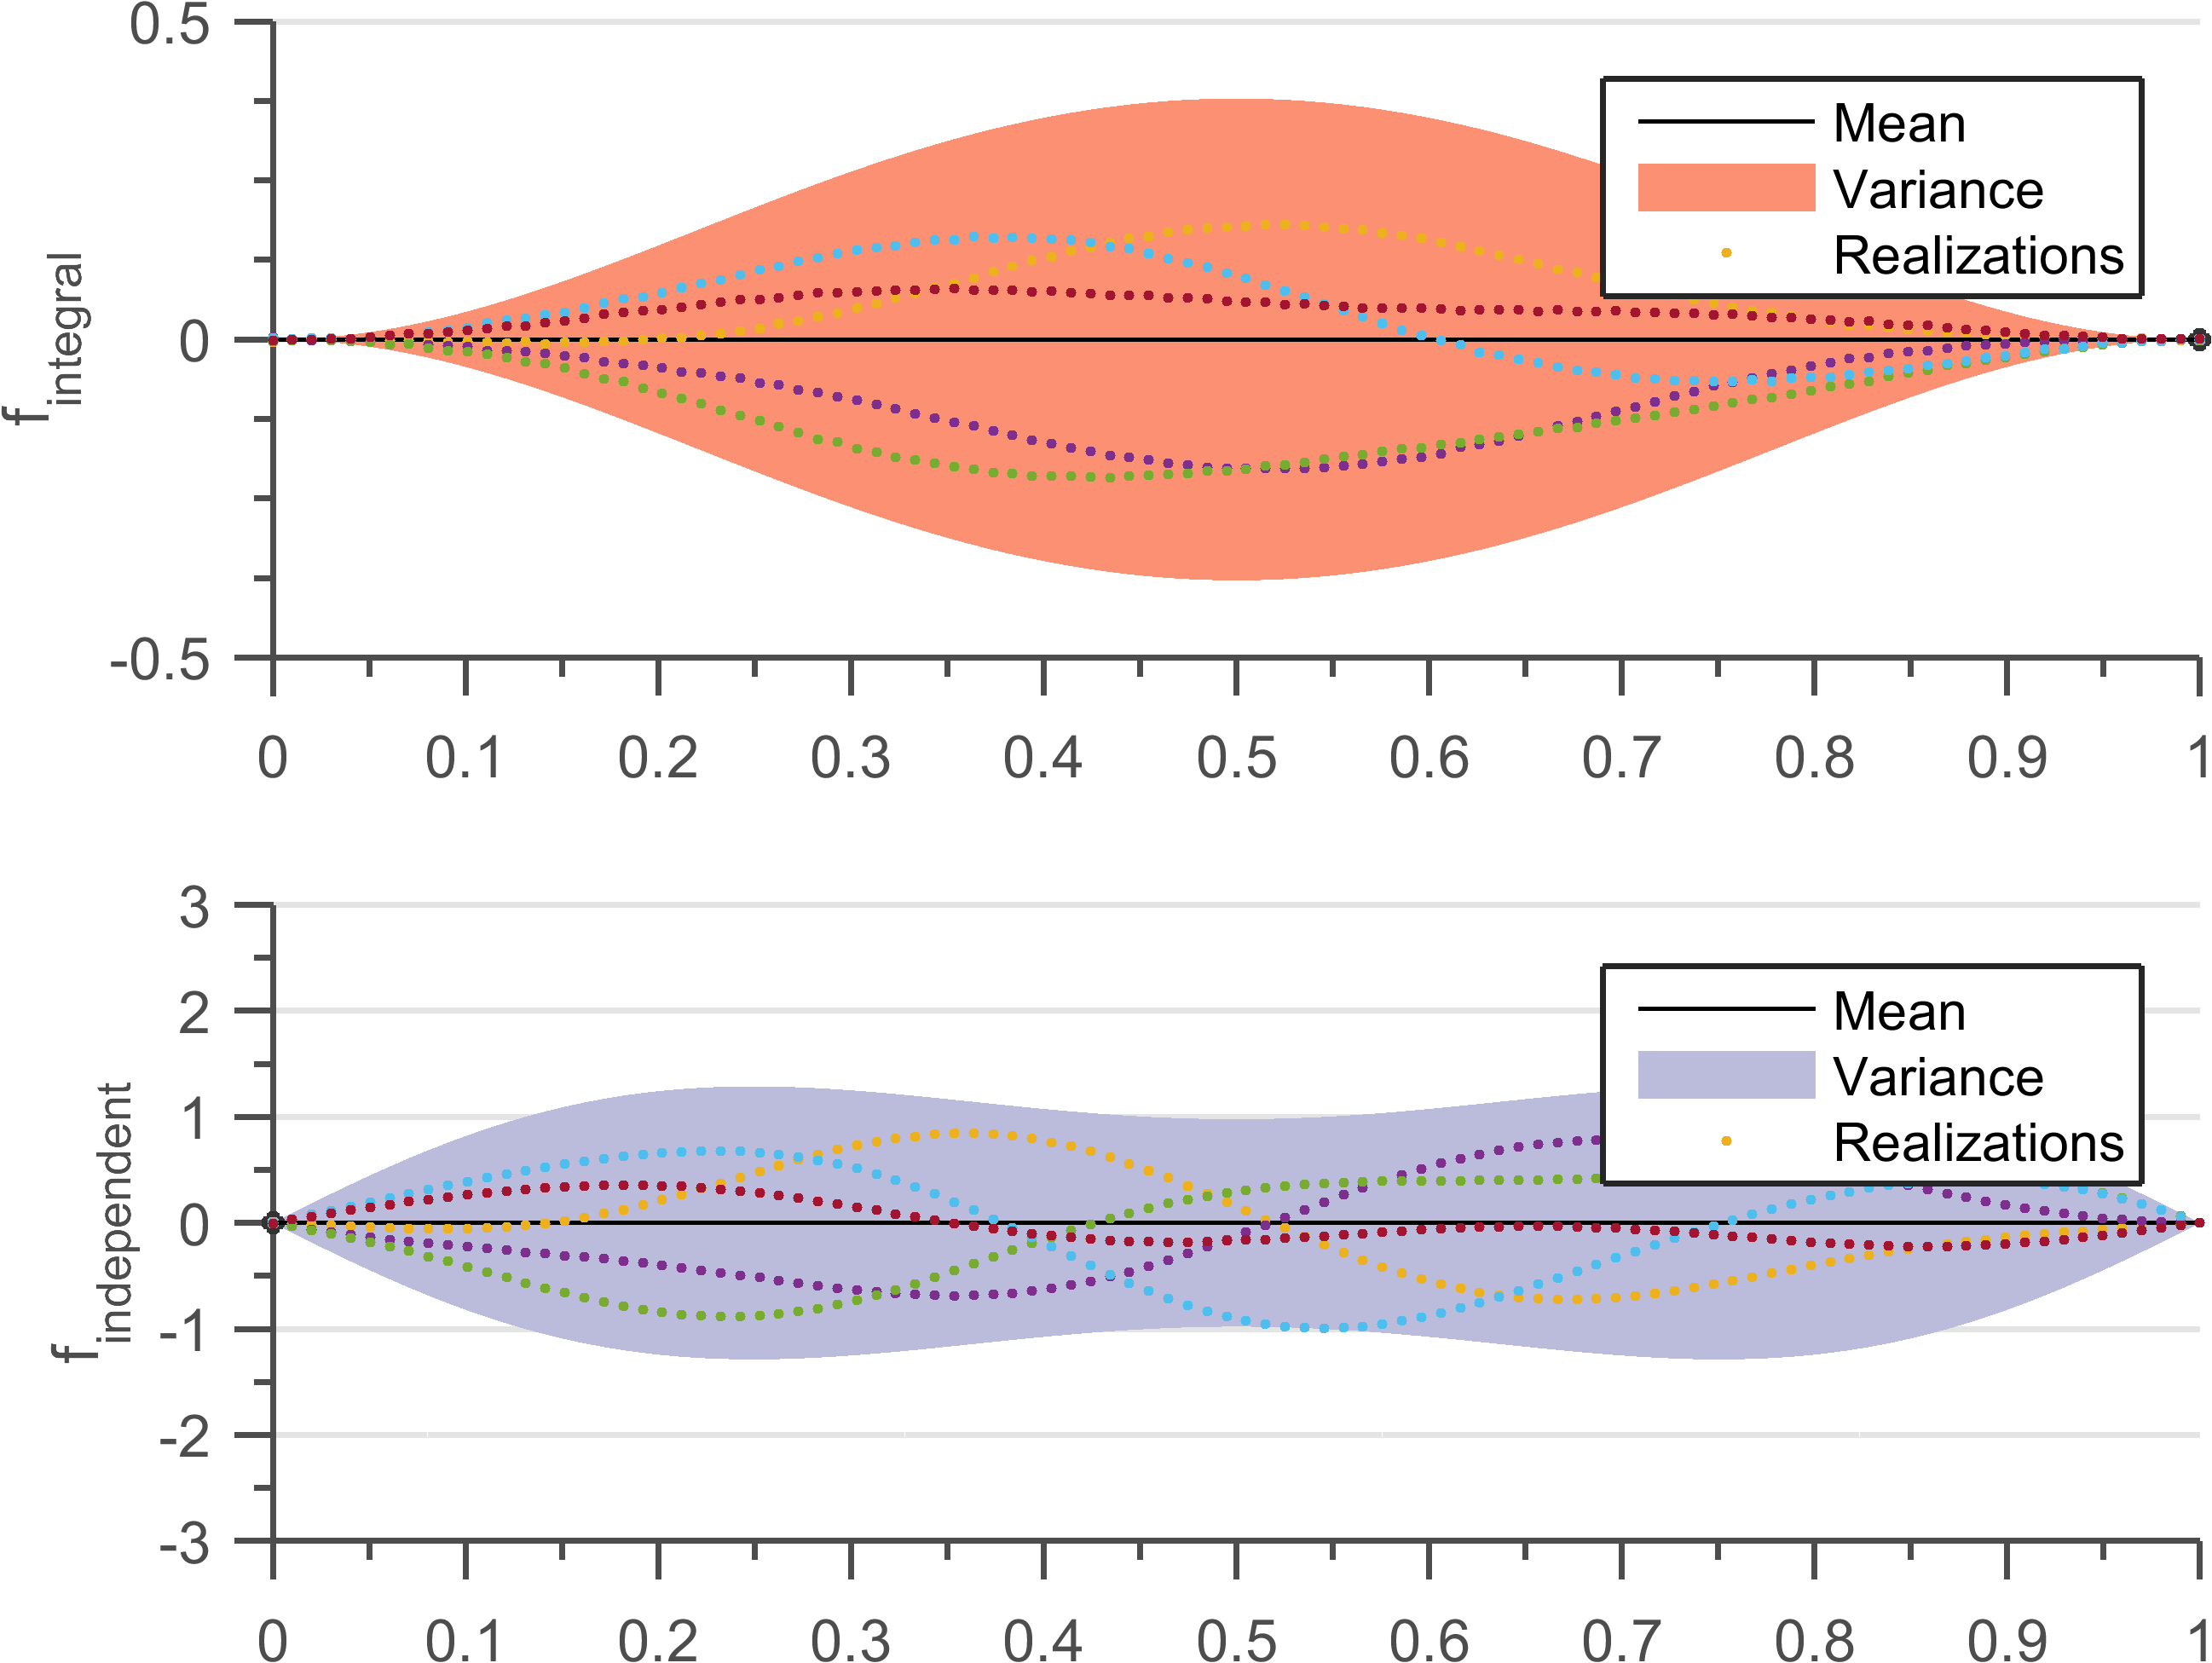
\includegraphics[width=0.485\textwidth]{images/drawsIntegralRelationship}\label{subfig:drawsIntegralRelationship}}
  \caption{Multi-Output Gaussian Process Regression Predictions}
\end{figure}

Here the hyperparameters of the prior are \(\theta = \left \{ l_{2}, \sigma_{2}^{2}, \sigma _{n1}^{2}, \sigma _{n2}^{2} \right \}\). These correspond to the hyperparameters of the independent covariance function \(K_{22}\) and errors in the measurements \(\sigma _{n1}^{2}\) and \(\sigma _{n2}^{2}\). Calculating the negative log-marginal likelihood involves inverting the matrix \(K_{XX} + \Sigma\). The size of the \(K_{XX} + \Sigma\) matrix depends on total number of input points \(N\), hence inverting the matrix becomes intractable for large number of input points.    

The fig: \ref{subfig:drawsDifferentialRelationship} shows mean and variance for a differential relationship between independent function \(f_{2}\) (blue) and differential function \(f_{1}\) (red) and such that \(f_{1} = \frac{\partial f_{2}}{\partial x}\). We have conditioned the two functions such that \(f_{1} = 5; x = 0\) and \(f_{2} = 0; x = 0\). This means that the function \(f_{2}\) passes through \(0\) and has a derivative equal to \(5\) at \(x = 0\). We have not maximized the marginal likelihood for this case and the hyperparameters of \(K_{22}\) are \(\theta_{1} = 1; \theta_{2} = 0.2\). All the corresponding draws from the posterior GP also follow the conditioning. 

The fig: \ref{subfig:drawsIntegralRelationship} shows mean and variance for a integral relationship between independent function \(f_{2}\) (blue) and differential function \(f_{1}\) (red) and such that \(f_{1} = \int f_{2} . dx\). We have conditioned the two functions such that \(f_{1} = 0; x = 1\) and \(f_{1} = 0; x = 0\). This means that the function \(f_{2}\) has an integral \(0\) at the two points \([0, 1]\) . We have not maximized the marginal likelihood for this case and the hyperparameters of \(K_{22}\) are \(\theta_{1} = 1; \theta_{2} = 0.2\). All the corresponding draws from the posterior GP also follow the conditioning. We can observe that the draws will also have an integral \(0\) between the range \([0, 1]\).

In the next section we describe how to solve the problem of inverting huge \(K_{XX} + \Sigma\) matrices using approximate inference techniques.

\section{Results}\label{sec:results}
In this section we provide numerical illustration to the theoretical derivations in the earlier sections. We start with a synthetic problem where we try to learn the model over quadratic relationships. We compare the cross-validation error values of independent GPR with that of multi-output joint GPR. Finally, we compare the performance of our methods on flight-loads estimation for horizontal tail plane.

The basic toolbox used for this paper is GPML provided with \cite{Rasmussen2005}, we generate covariance functions to handle relationships as described in equations \ref{eq:exactJointCovariance} and \ref{eq:approxJointCoariance} using the ''Symbolic Math Toolbox" in MATLAB 2014b. All experiments were performed on an Intel quad-core processor with 4Gb RAM.

\subsection{Quadratic relation on Synthetic Data}\label{sub:experimentsSyntheticData}
We take the case of a quadratic operator \(g(.)\) equation \ref{eq:quadraticRelationship}. 
\begin{equation}\label{eq:quadraticRelationship}
f_{1} = f_{2}^2
\end{equation}

To generate the data we randomly draw a single function of \(f_{2}\) as described in equation \ref{eq:experimentalSET} for 50 equally spaced inputs between [-1, 1]. The data for \(f_{1}\) is the calculated using equation \ref{eq:quadraticRelationship}. The latent functions \(f's\) are then corrupted according to equation \ref{eq:experimentalSET} which gives us the outputs \(y's\). We finally hide the observations for \(y_{1}\) in the domain \(x = [-0.2, 0.2]\). We thus have our dataset for testing the performance of quadratic relationship. 

\begin{equation*}
f_{2} \sim  GP[0, K_{SE}(0.2, 1)]
\end{equation*}
\begin{equation*}
\sigma_{n2} \sim \mathcal{N}[0, 0.1]
\end{equation*}
\begin{equation}\label{eq:experimentalSET}
\sigma_{n1} \sim \mathcal{N}[0, 1]
\end{equation}
     
\(K_{SE}(0.2, 1)\) means squared exponential kernel with length scale 0.1 and variance as 1. \(\sigma_{n2}\) and \(\sigma_{n1}\) are the white noises added to the latent functions \(f_{1}\) and \(f_{2}\) respectively. Since the quadratic relationship \(g(.)\) is non-linear in nature we use the equation \ref{eq:approxJointCoariance} to calculate the auto- and cross-covariance functionsas explained in equation \ref{eq:jointKernelForQuadratic relationship}. 

\begin{equation*}
K_{12} = 2\mu_{y_{2}}(x_{1})K_{22}
\end{equation*}
\begin{equation}\label{eq:jointKernelForQuadratic relationship}
K_{11} = 4\mu_{y_{2}}(x_{1})^2K_{22}
\end{equation}

Here, \(\mu_{y_{2}}(x_{1})\) is the mean value of function \(y_{2}\) calculated at the input points \(x_{1}\). For the case of quadratic relationship the jacobian \(L\) as described in equation \ref{eq:approxJointCoariance} comes out to be \(2*\mu_{y_{2}}(x_{1})\). For non-linear operators \(g(.)\) the joint-covariance prior is depends on the mean value of \(f_{2}\). \(K_{22}\) and \(K_{11}\) are the auto-covariance functions calculated at the input points \(x_{1}\) and \(x_{2}\) as described in equation \ref{eq:approxJointCoariance} and equation \ref{eq:mogpJointPrior}. \(K_{12}\) is the cross-covariance function between the input points \(x_{1}\) and \(x_{2}\). We can observe that the joint-covariance has been expressed as a function of covariance \(K_{22}\) using equation \ref{eq:quadraticRelationship}.  

\begin{figure}[!t]
  \centering
  
  \subfigure[{Independent GP Regression for the two outputs \(y_{1}\) and \(y_{2}\). The solid black line represents the predicted mean while the shaded area denotes 1\(\sigma\) uncertainity region. The dashed black line represents the real value of \(f_{1}\). For \(y_{1}\) the data is hidden from section \(x = [-0.2, 0.2]\). We can observe the huge difference between the real data and the predicted mean values at zone with no data.}]
  {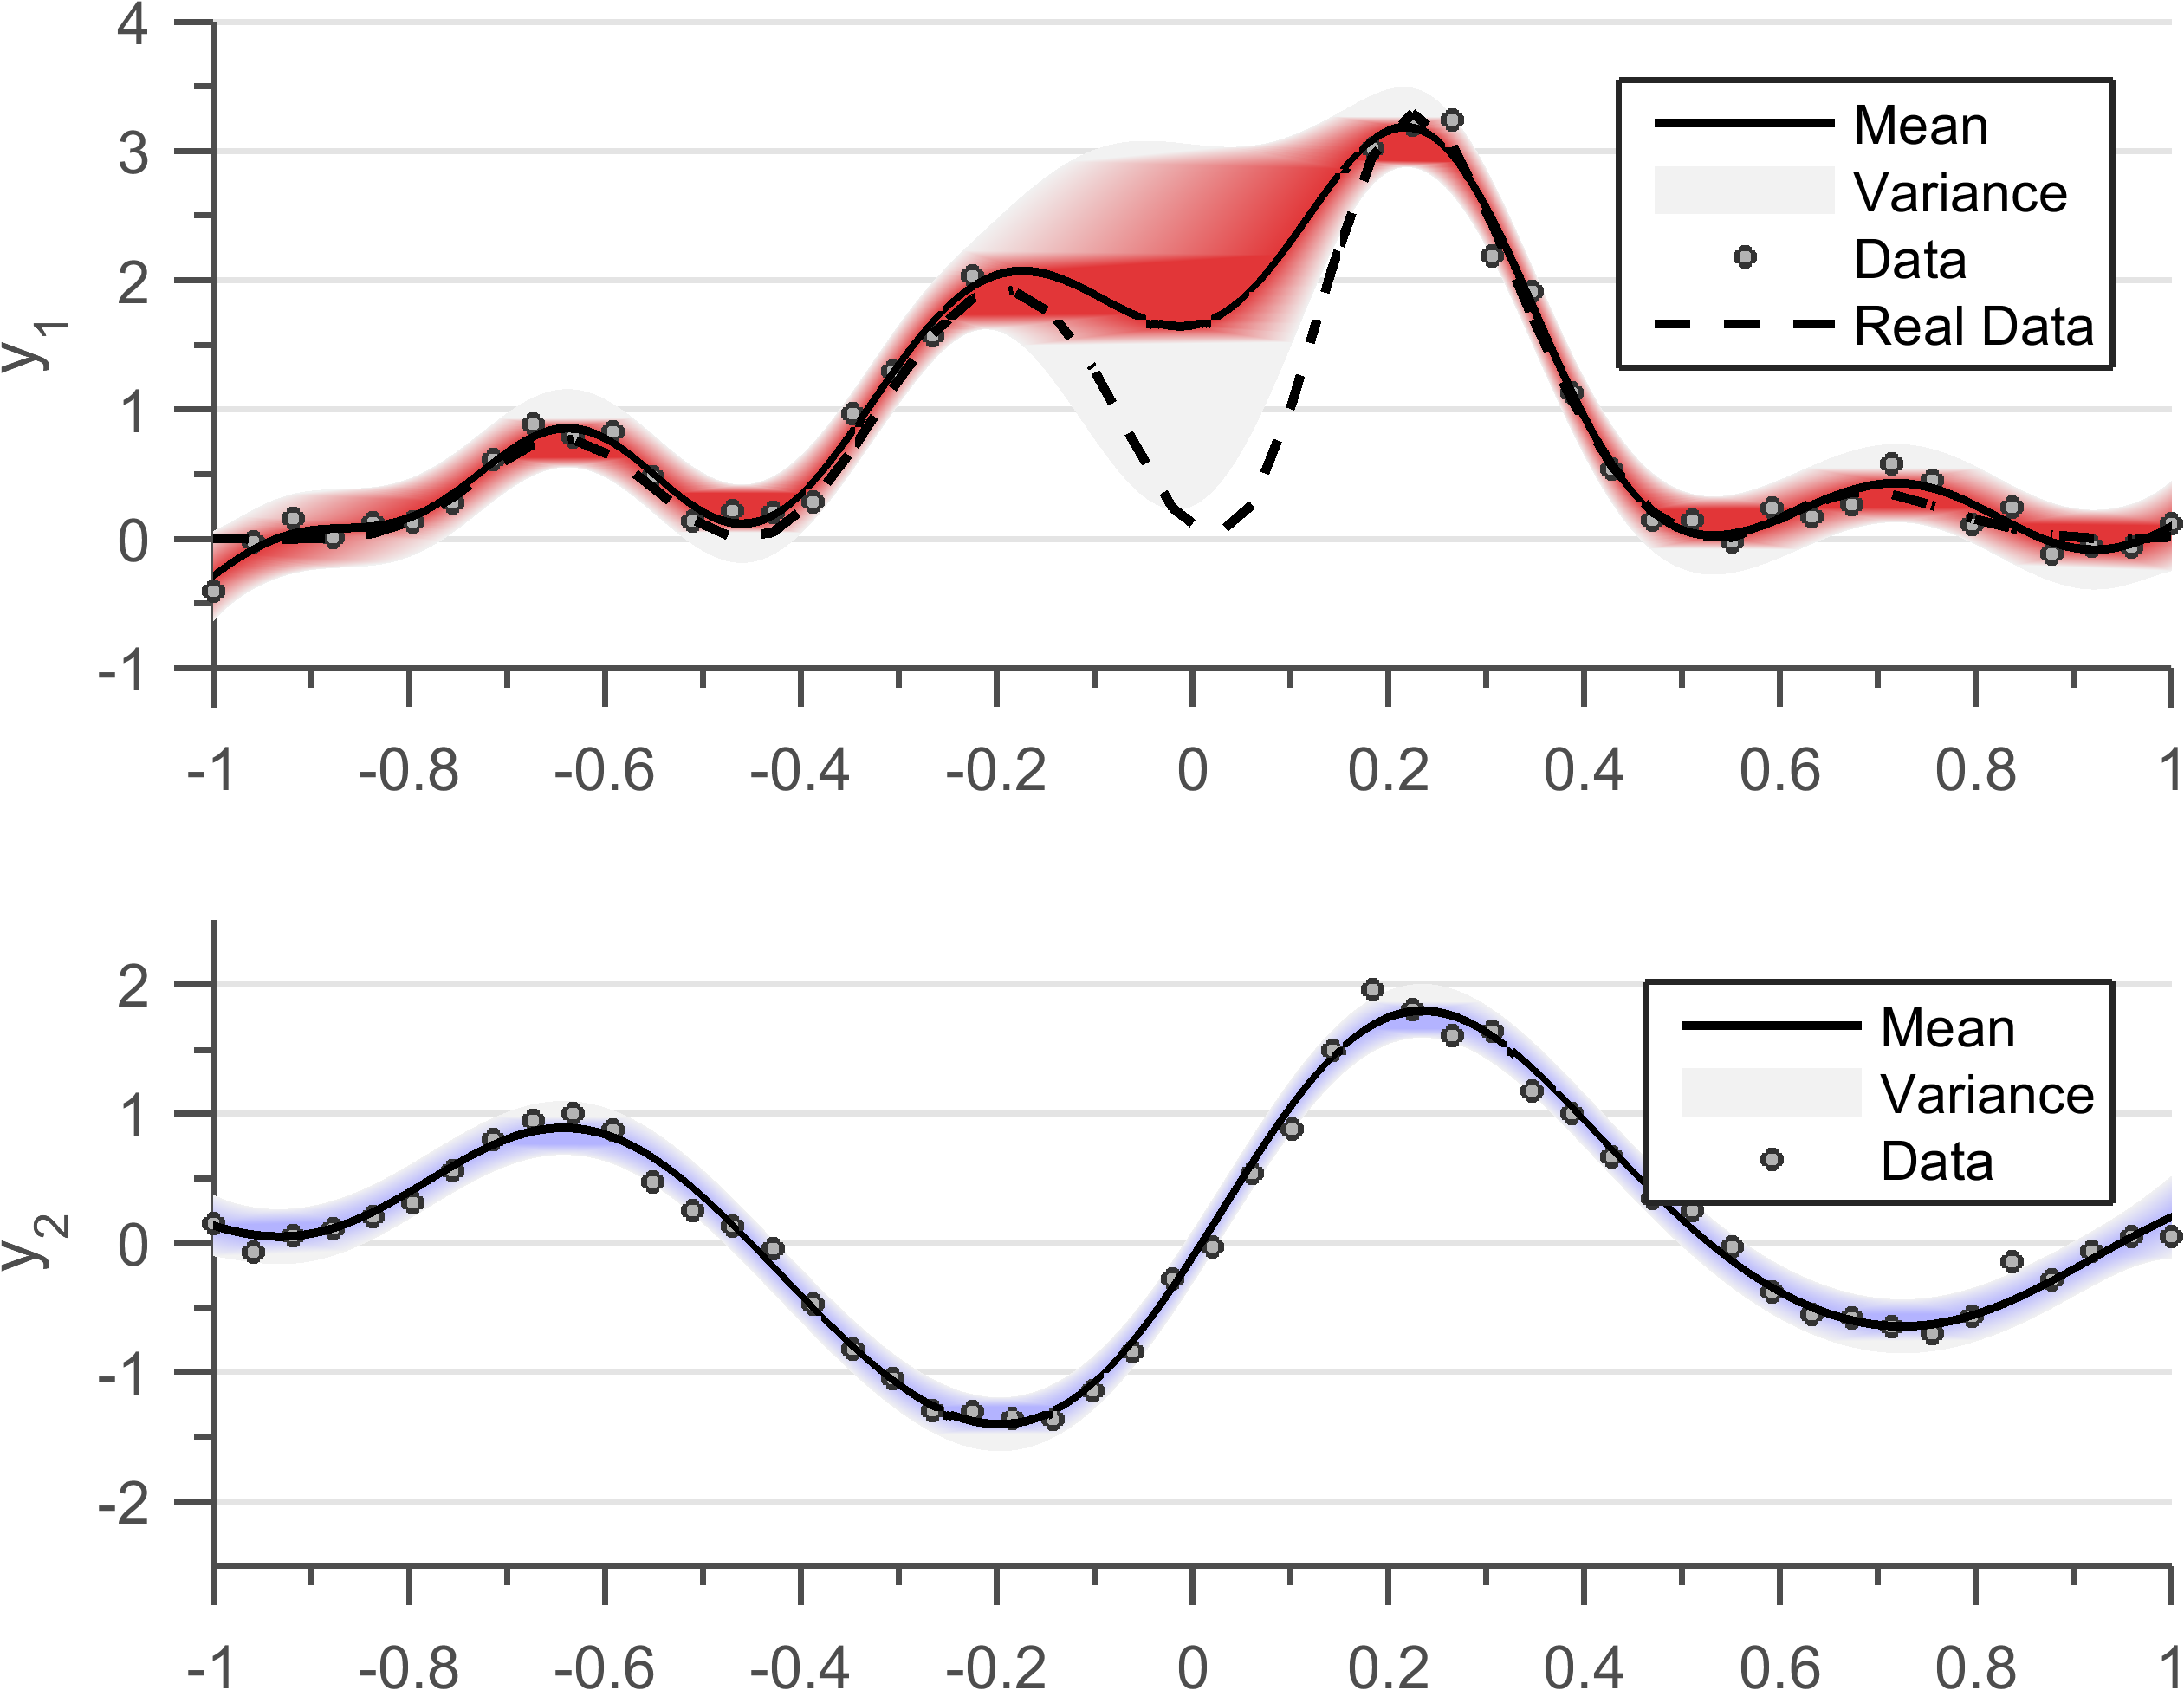
\includegraphics[width=0.45\textwidth]{images/quadraticRelationshipIndependent}
  \label{subfig:quadraticRelationshipIndependent}}\quad
  
  \subfigure[{Joint-GP Regression for the two outputs \(y_{1}\) and \(y_{2}\) related through equation \ref{eq:quadraticRelationship}. The solid black line represents the predicted mean while the shaded area denotes 1\(\sigma\) uncertainity region. The dashed black line represents the real value of \(f_{1}\). For \(y_{1}\) the data is hidden from section \(x = [-0.2, 0.2]\). We can observe the improved prediction between zone with no data because information is being shared between the two outputs.}]
  {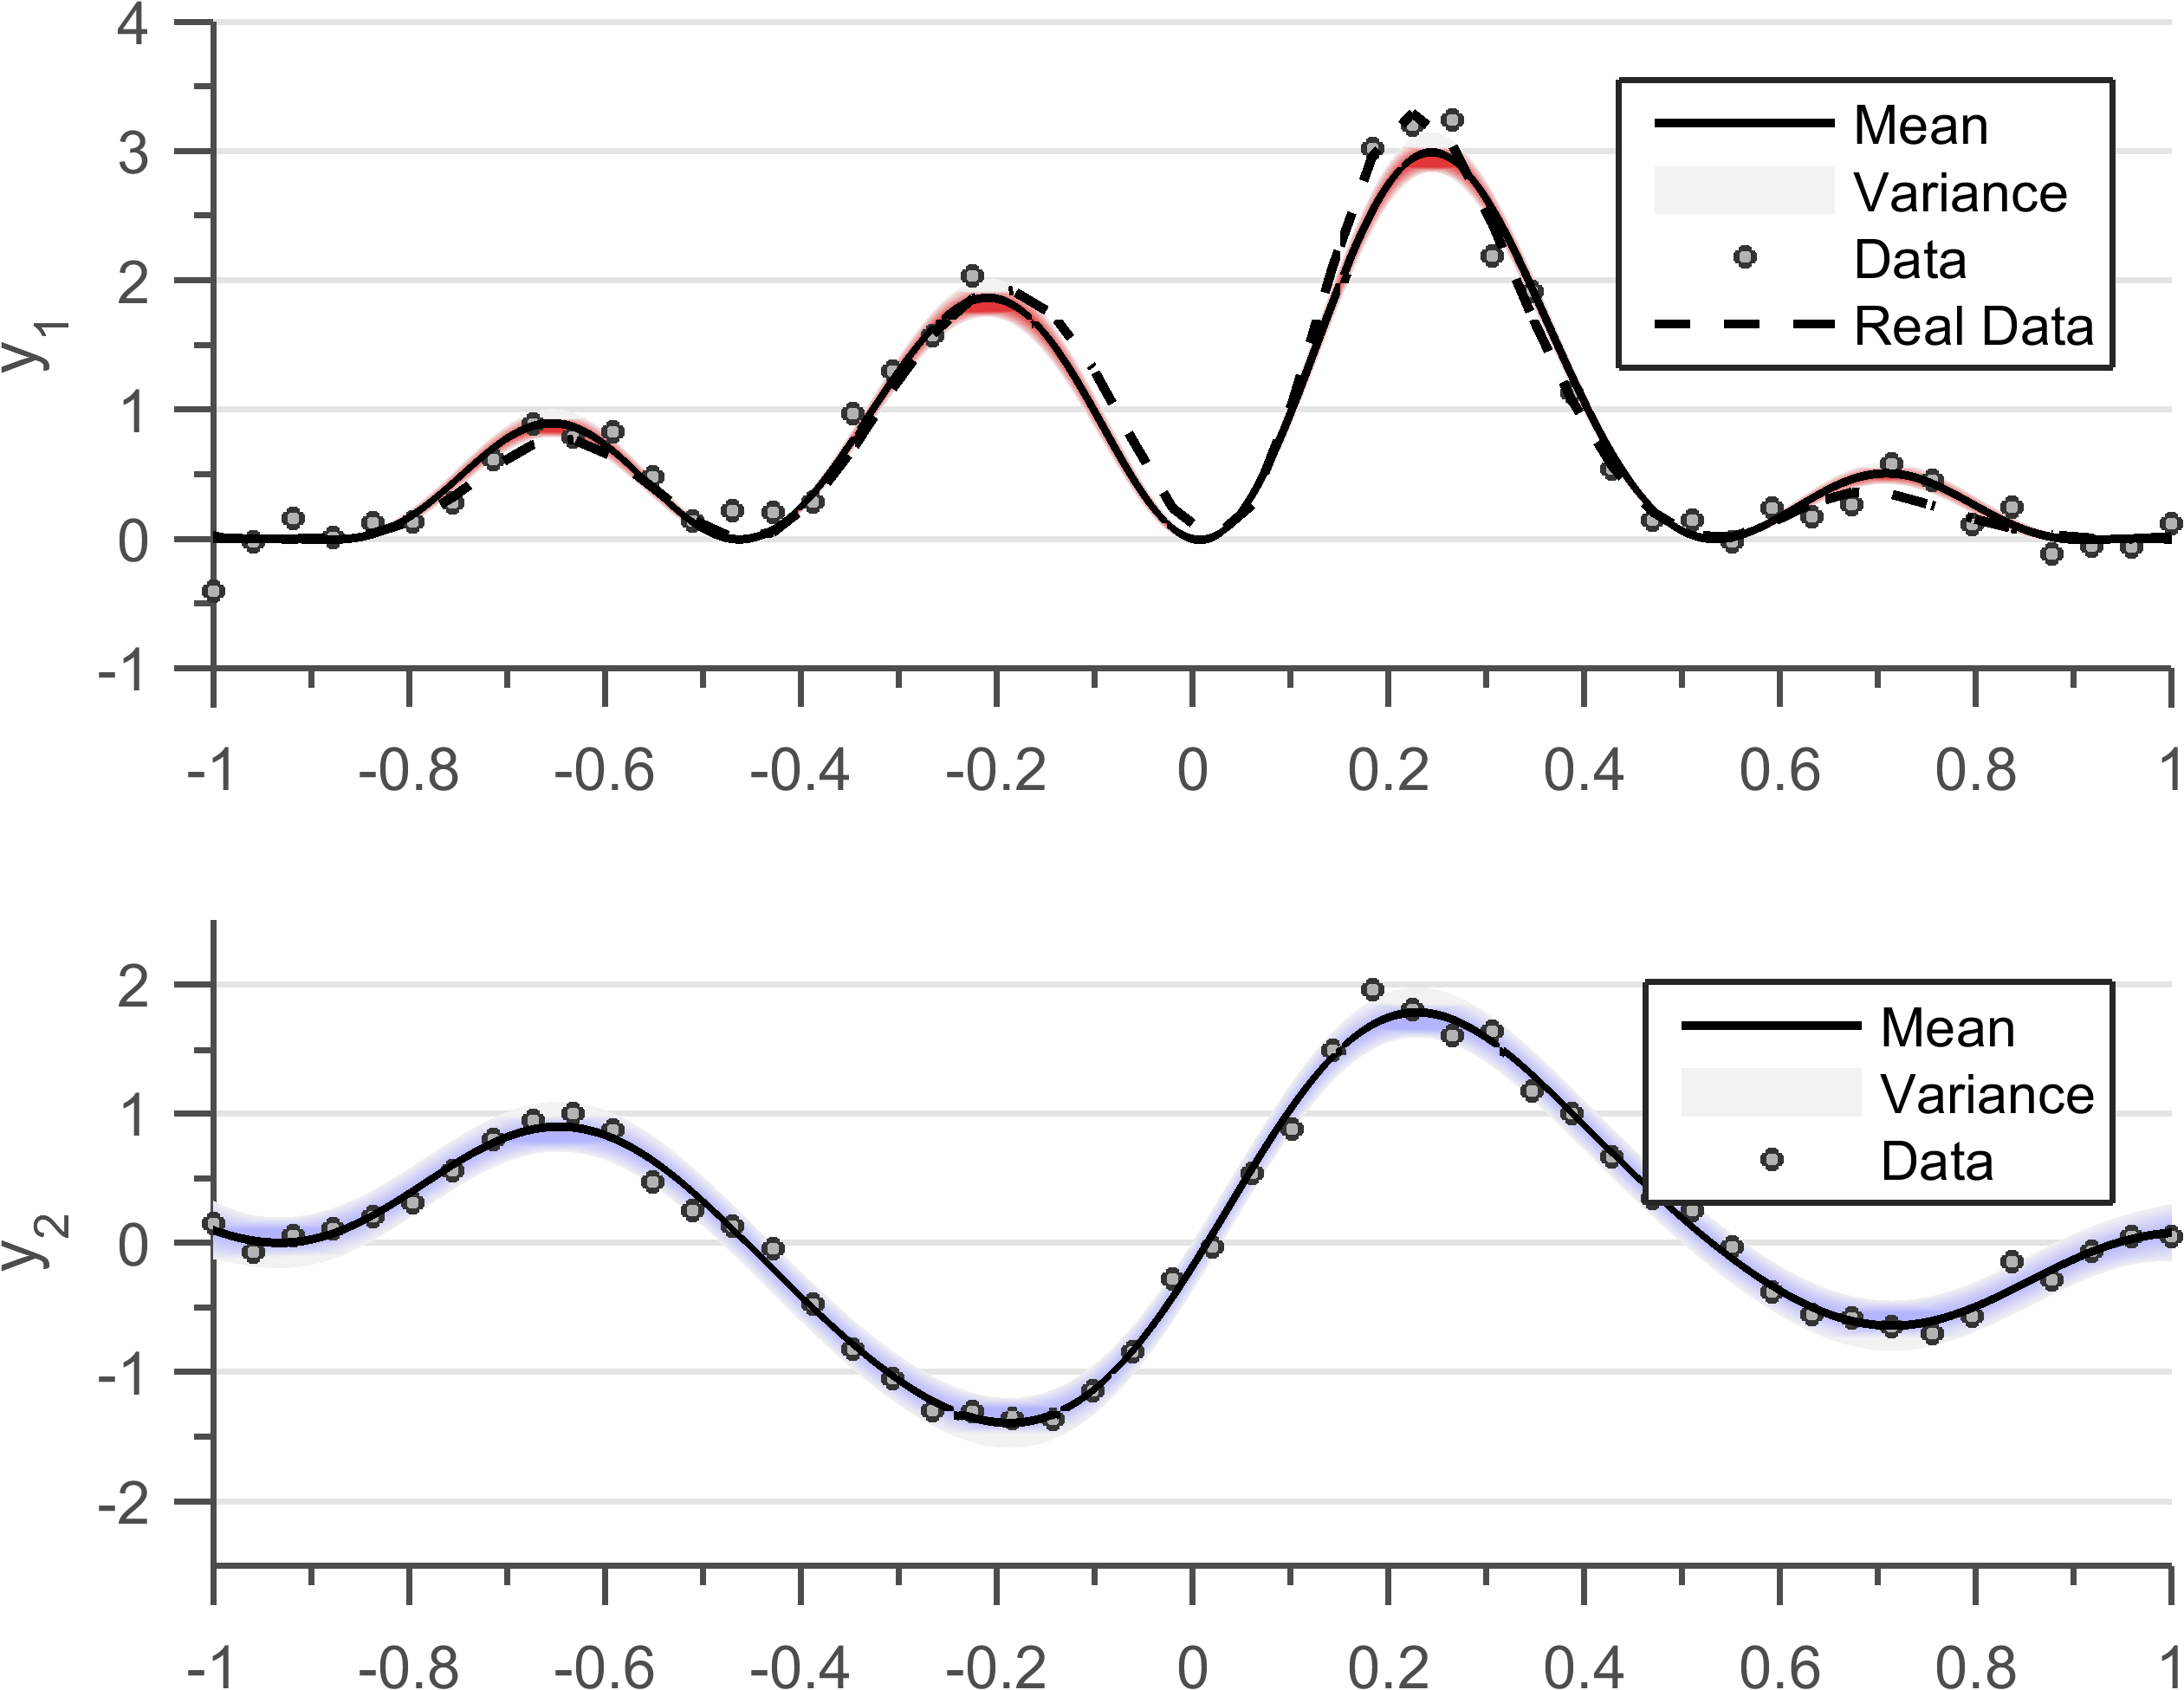
\includegraphics[width=0.45\textwidth]{images/quadraticRelationshipJointKernel}
  \label{subfig:quadraticRelationshipJointKernel}}
  
  \caption{GP Regression on Quadratic relationship}
\end{figure}\label{fig:GPMOQuadraticRelationship}


Figure \ref{subFigquadraticRelationshipIndependent} shows the independent fit of two GPR. For the case of \(y_{1}\) there is a huge difference between the real data and predicted mean at points where data is unavailable. Figure \ref{subFigquadraticRelationshipJointKernel} shows the joint-GP regression. Joint-GP model gives better prediction even in the absence of data for \(y_{1}\) because transfer of information is happening from observations of \(y_{2}\) present at those locations. For the case of \(y_{2}\) there is no significant improvement in the prediction of two methods. 

\begin{table}
\caption{mean RMSE errors for quadratic relationship}
\centering
\label{t:observed_psrs}
\begin{tabular}{rcc}
\noalign{\smallskip} \hline \hline \noalign{\smallskip}
 & RMSE \(y_{1}\) & RMSE \(y_{2}\) \\
\hline
Independent Single-output GPR & 1.74 & 0.14 \\
Joint Multi-output GPR & 0.26 & 0.12 \\
\noalign{\smallskip} \hline \noalign{\smallskip}
\end{tabular}
\label{table:rmseY1Y2}
\end{table}

Table \ref{table:rmseY1Y2} shows comparison of Root Mean Square Error (RMSE). 10 sets of experiments were run for 85\% of data as training set and 15\% of data as test set, the training and test sets were chosen randomly. We learn the optimal set of hyperparameters for on training data all 10 sets of experiments. Finally RMSE values are evaluated with respect to the test set. We see a significant improvement in performance for the case of joint multi-output GPR. 

\subsection{Flight Mechanics on Flight Test Data}\label{sub:experimentsFlightLoadsData}
Procuring data in engineering design is a costly exercise, a high-fidelity CFD simulation runs for days and a flight test campaign costs millions. In this context it is important to be data efficient while creating models with data. We leverage the knowledge of available relations between several data and 


In this section we conduct experiments, applying our approach on the flight loads data. We look at normalized data of a simple longitudinal maneuver. The maneuver is quasi-static which means that airplane is in equilibrium at all times and there are no dynamic effects observed by the aircraft. The two outputs in our case are coefficient of lift \(C_{z}\) on the Horizontal Tail Plane (HTP) and spanwise lift \(k_{z}\). We know that the integral of spanwise pressure will be equal to the coefficient of lift.

\begin{equation}\label{eq:relationCzKz}
\centering
C_{z}(\eta) = \int_{\eta_{edge}}^{\eta_{root}} k_{Z}(\eta)d\eta
\end{equation}.

Here, \(\eta_{edge}\) denotes the edge of horizontal tail span while \(\eta_{root}\) represents root of tail. The above equation is linear in nature and hence we will use equation \ref{eq:exactJointCovariance} to calculate the auto- and cross-covariance functions.

In practice, the coefficient of lift \(C_{z}\) is calculated using strain gauges on the HTP and the spanwise force is measured using pressure tappings. Chordwise pressures are measured at multiple \(\eta\) locations on the HTP, which are integrated chordwise to give spanwise lift distribution. We are trying to merge data coming from two different calculation chains flight mechanics and aerodynamics using a basic physics based relation and improve the performance of our model.

\begin{figure}[!ht]
  \centering
  \subfigure[{Joint multi-output GPR between \(K_{z}\) and \(C_{z}\) using a SE kernel and equation \ref{eq:relationCzKz}.}]
  {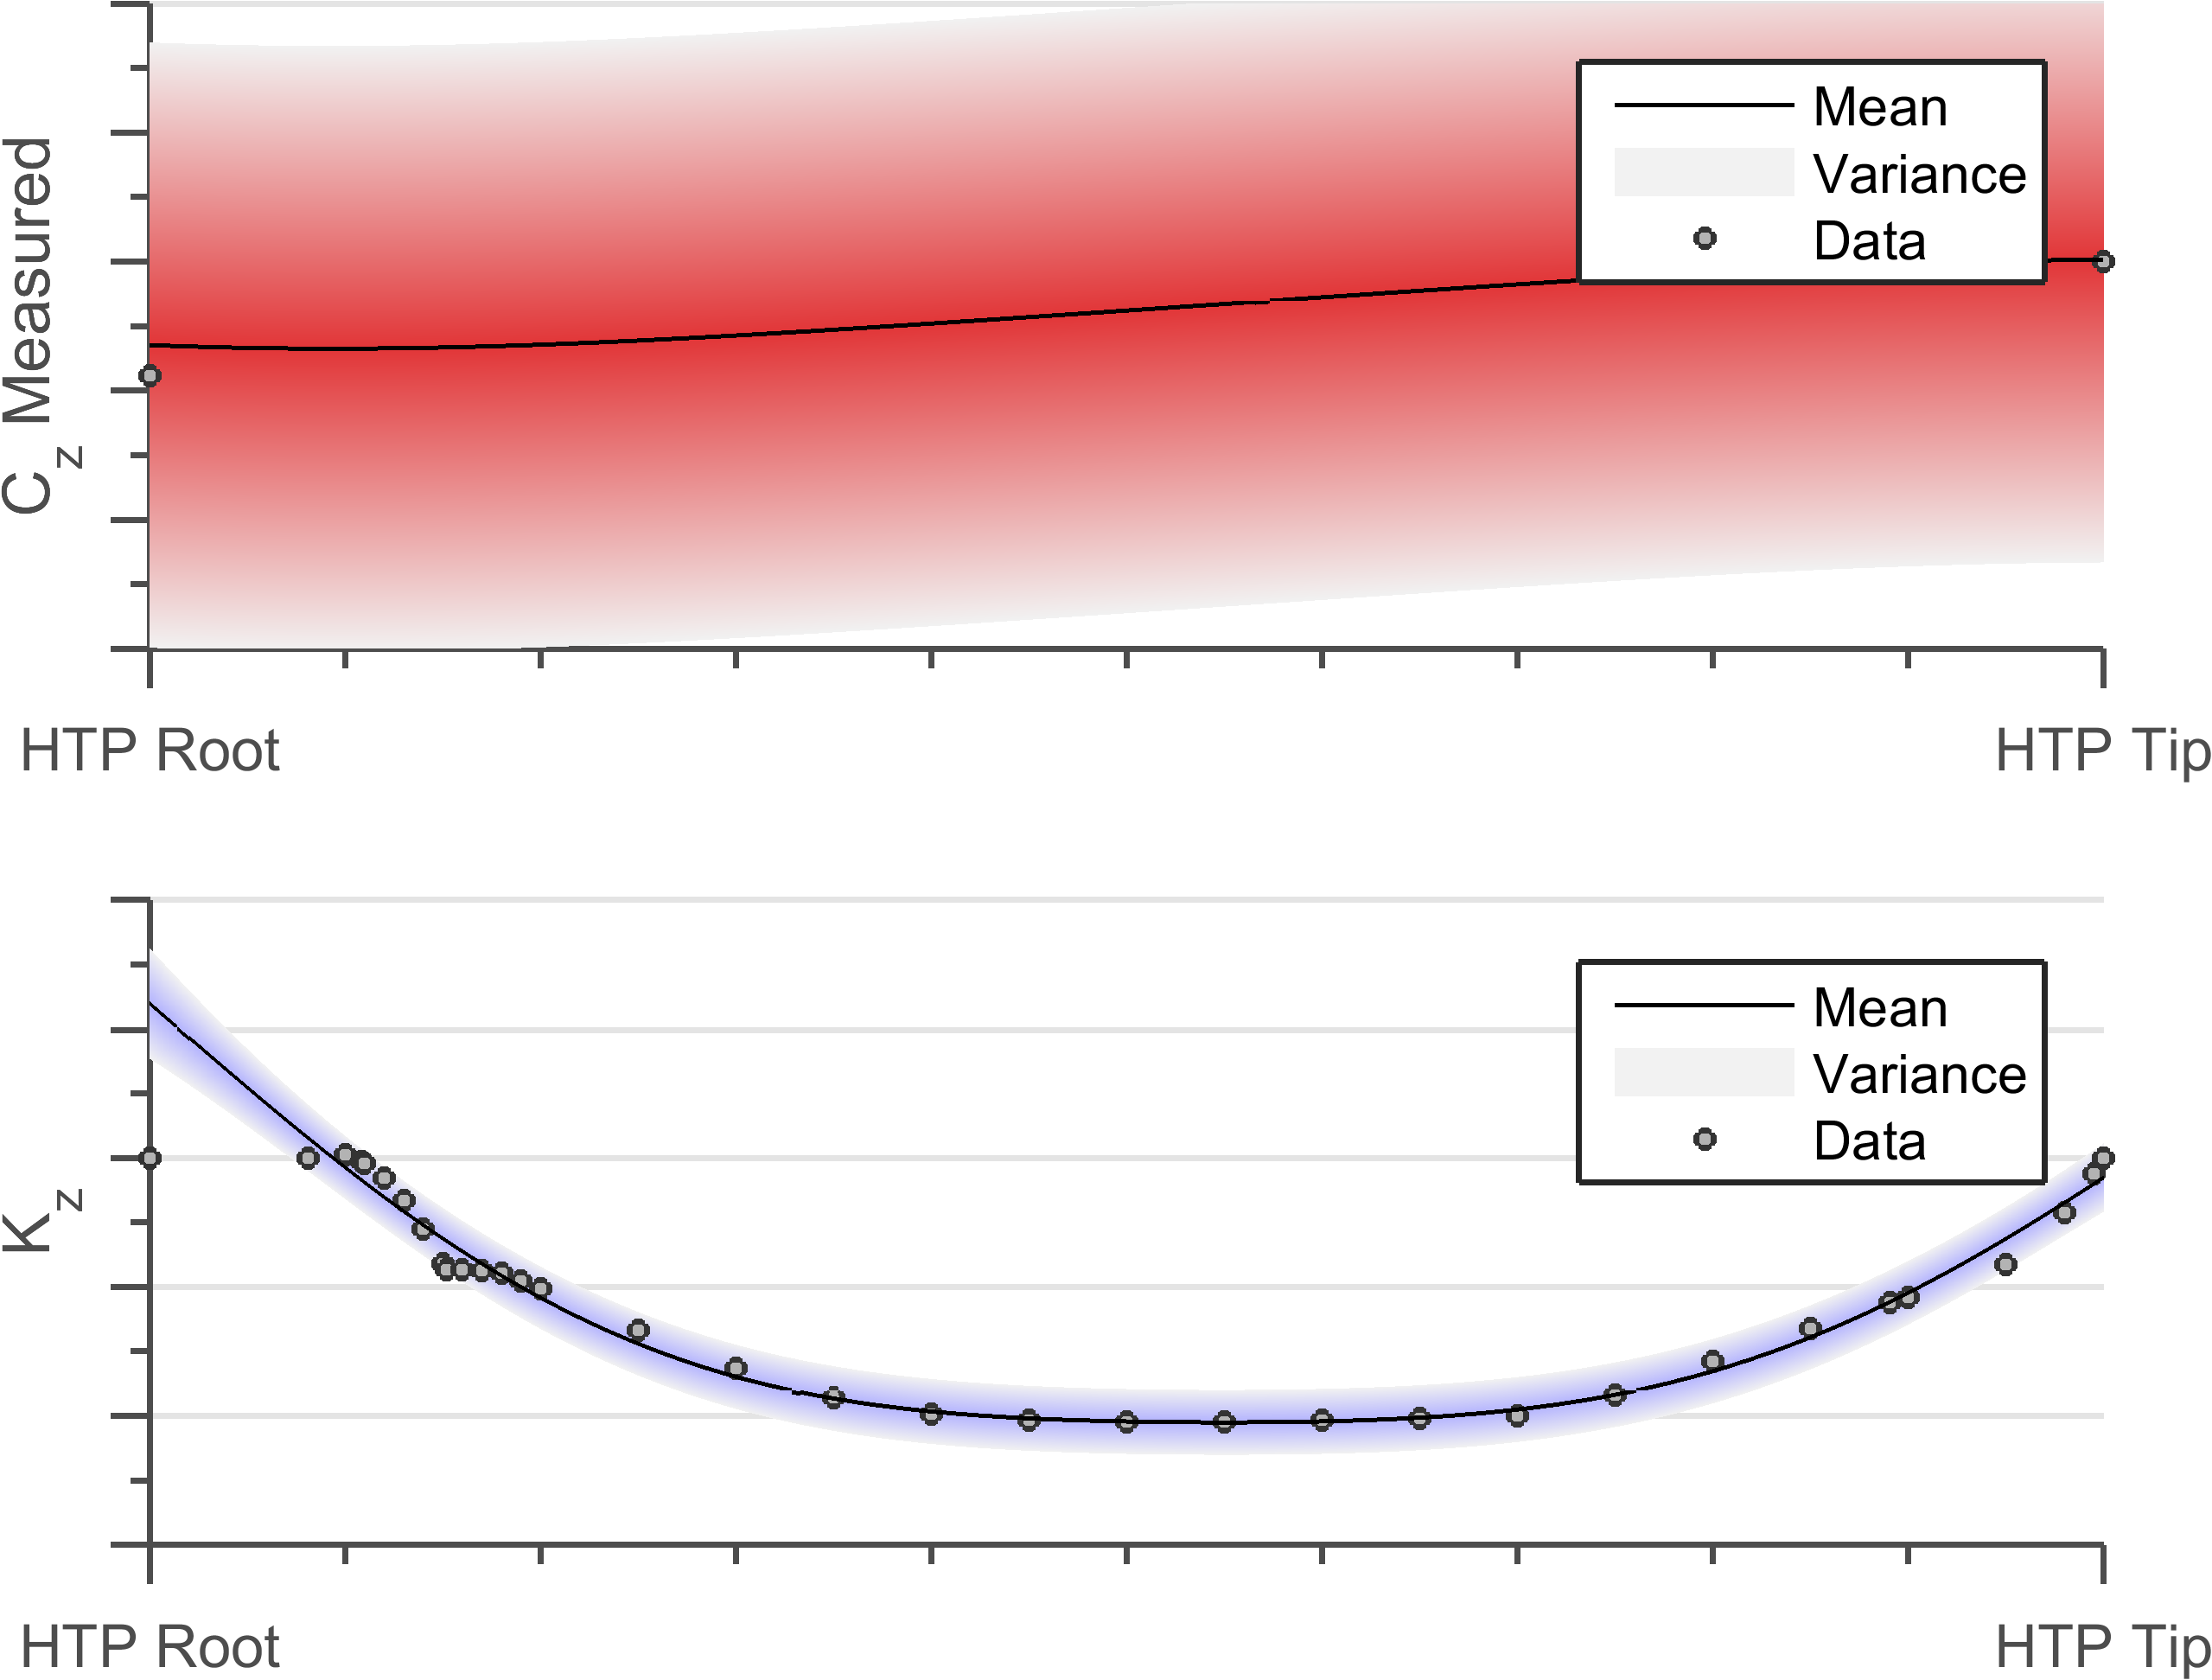
\includegraphics[width=0.45\textwidth]{images/KLPreFlightAndCzPreFlight_200_SE}\label{subfig:KLPreFlightAndCzPreFlight_200_SE}}\quad
  
  \subfigure[{Joint multi-output GPR between \(K_{z}\) and \(C_{z}\) using a twice differentiable Mat\'ern kernel and equation \ref{eq:relationCzKz}.}]
  {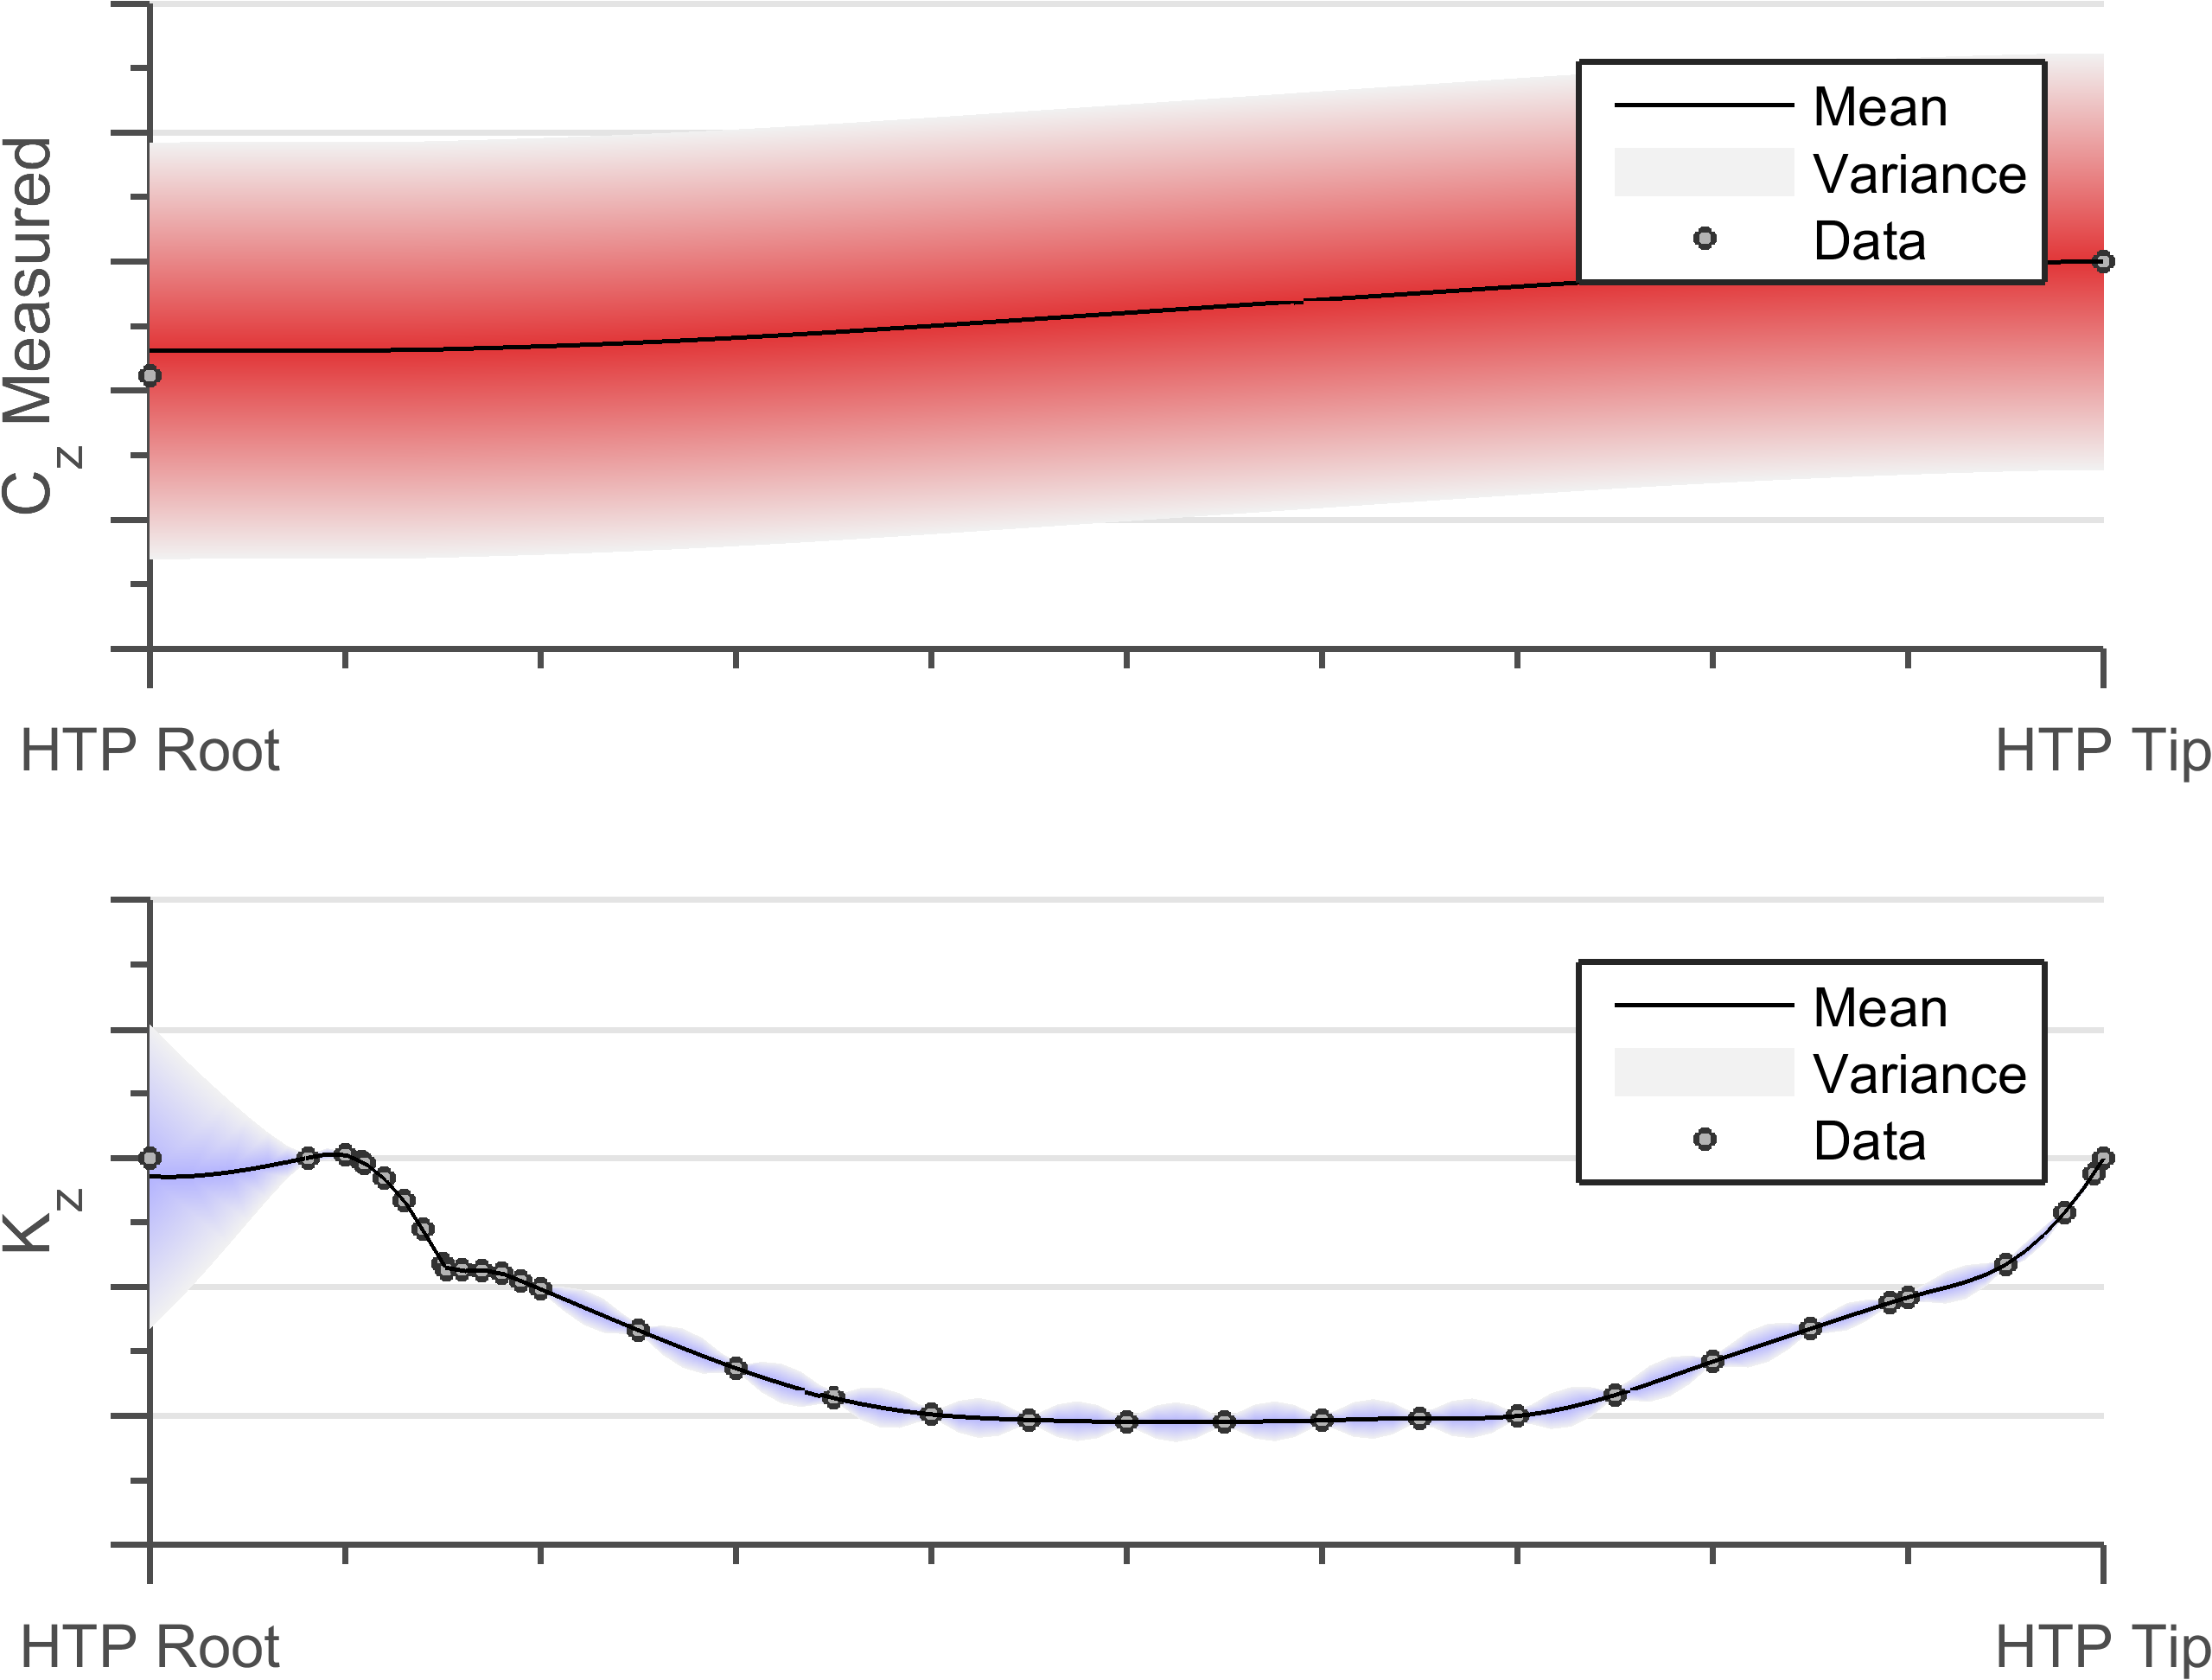
\includegraphics[width=0.45\textwidth]{images/KLPreFlightAndCzPreFlight_200_MAT5}\label{subfig:KLPreFlightAndCzPreFlight_200_MAT5}}
  \caption{Joint multi-output GPR on  \(K_{z}\) and \(C_{z}\) relationship}\label{fig:cztzRelationship}
\end{figure}


Figure \ref{fig:cztzRelationship} shows a comparison between two joint multi-output GPR on \(K_{z}\) and \(C_{z}\) using initial assumptions regarding order of differentiability. Figure \ref{subFigKLPreFlightAndCzPreFlight_200_SE} shows the effect of SE kernel (infinite differentiability) on the joint model. The SE kernel is a strong assumption for type of lift distribution. To accomodate for the value of measured \(C_{z}\) the error band increases and the boundary condition at HTP root is not satisfied. Moreover, we identify points in the figure \ref{subFigKLPreFlightAndCzPreFlight_200_SE} which fall out of the 95\% confidence band. We can claim with 95\% probability that if our lift distributions come from a family of highly differentiable functions these outliers do not satisfy the physics of the problem and can be termes as measurement errors.

Figure \ref{subFigKLPreFlightAndCzPreFlight_200_MAT5} shows the effect of twice differentiable Mat\'ern kernel on the joint model. The twice differentiable assumption gives our family of functions enough flexibility to follow the spanwise lift data. We observe that error estimates for \(C_{z}\) improves considerably while there is an increased uncertainity at the HTP root for \(K_{z}\). This loss in order of differentiability can be explained due to fuselage HTP interaction near HTP root. We can conclude that even though we are working with very basic assumptions of differentiability the choice of kernel is important in performing the predictions. 


\section{Approximating Inference}\label{sec:sparseGPRegression}
\noindent The above GP approach is intractable for large datasets. For a multi-output GP as defined in section \ref{sub:MOGPs} the covariance matrix is of size \(N\),  where \(\mathcal{O}\left ( N^{3} \right )\) time is needed for inference and \(\mathcal{O}\left ( N^{2} \right )\) memory for storage. Thus, we need to consider approximate methods in order to deal with large datasets. 

Inverting the covariance matrix takes considerable amount of time and memory during the process. Hence, almost all techniques to approximate inference try and approximate the inversion of covariance matrix \(K_{XX}\). If a covariance matrix is diagonal or block-diagonal in nature then methods such as mixture of experts are used eg. distributed GP. Whereas if the covariance matrix is more spread out and has similar terms in its cross diagonals then low-rank approximations are used eg. variational approximation. The remaining section details the two methods for approximating covariance matrix which can be later used to resolve equations \ref{eq:predictiveMOMean}, \ref{eq:predictiveMOCovariance} and \ref{eq:gradientNLML}.

\subsection{Variational Approximation on Multi-output GP}\label{sec:varMOGP}
Sparse methods use a small set of \(m\) function points as support or inducing variables. Suppose we use \(m\) inducing variables to construct our sparse GP. The inducing variables are the latent function values evaluated at inputs \(x_{M}\). Learning \(x_{M}\) and the hyperparameters \(\theta\) is the problem we need to solve in order to obtain a sparse GP method. An approximation to the true log marginal likelihood in equation \ref{eq:exactMONLML} can allow us to infer these quantities.

\begin{figure}[!t]
  \centering
  \subfigure[Full multi-output covariance matrix for fig: \ref{subfig:drawsIntegralRelationship}]
  {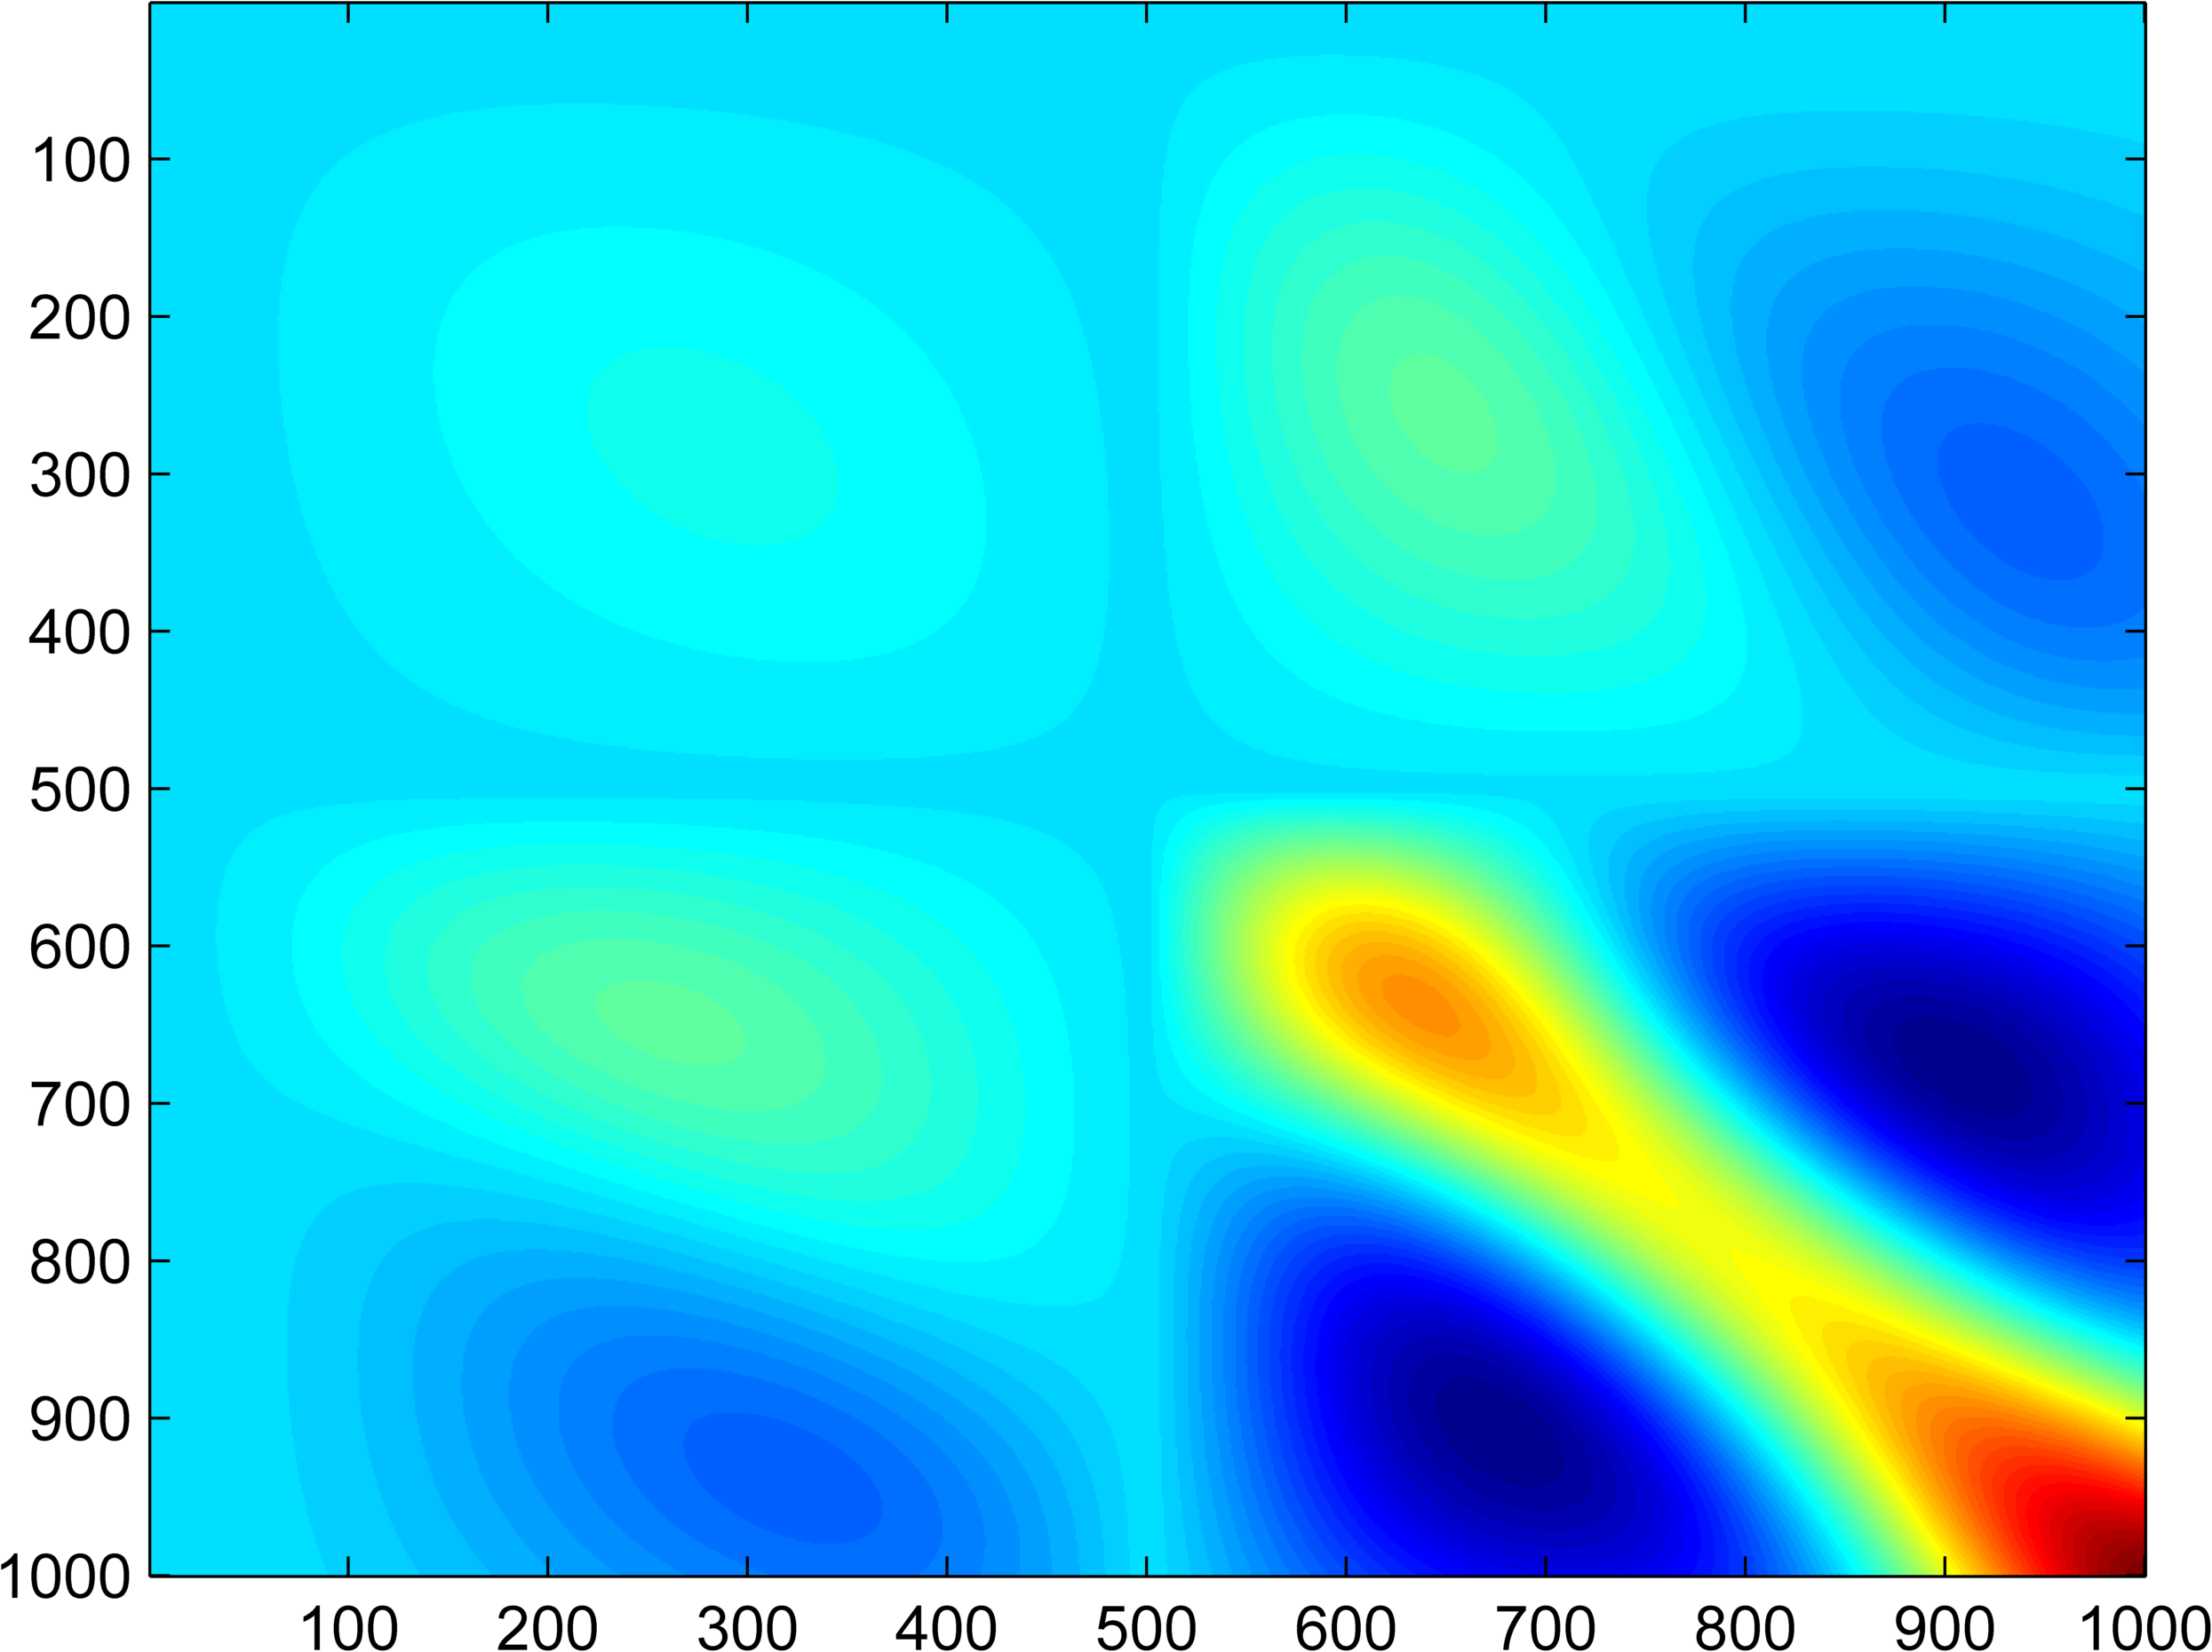
\includegraphics[width=0.45\textwidth]{images/kPredMultipleOutputIntegral}\label{subfig:kPredMultipleOutputIntegral}}\quad
  \subfigure[Approximated multi-output covariance matrix for fig: \ref{subfig:drawsIntegralRelationship}]
  {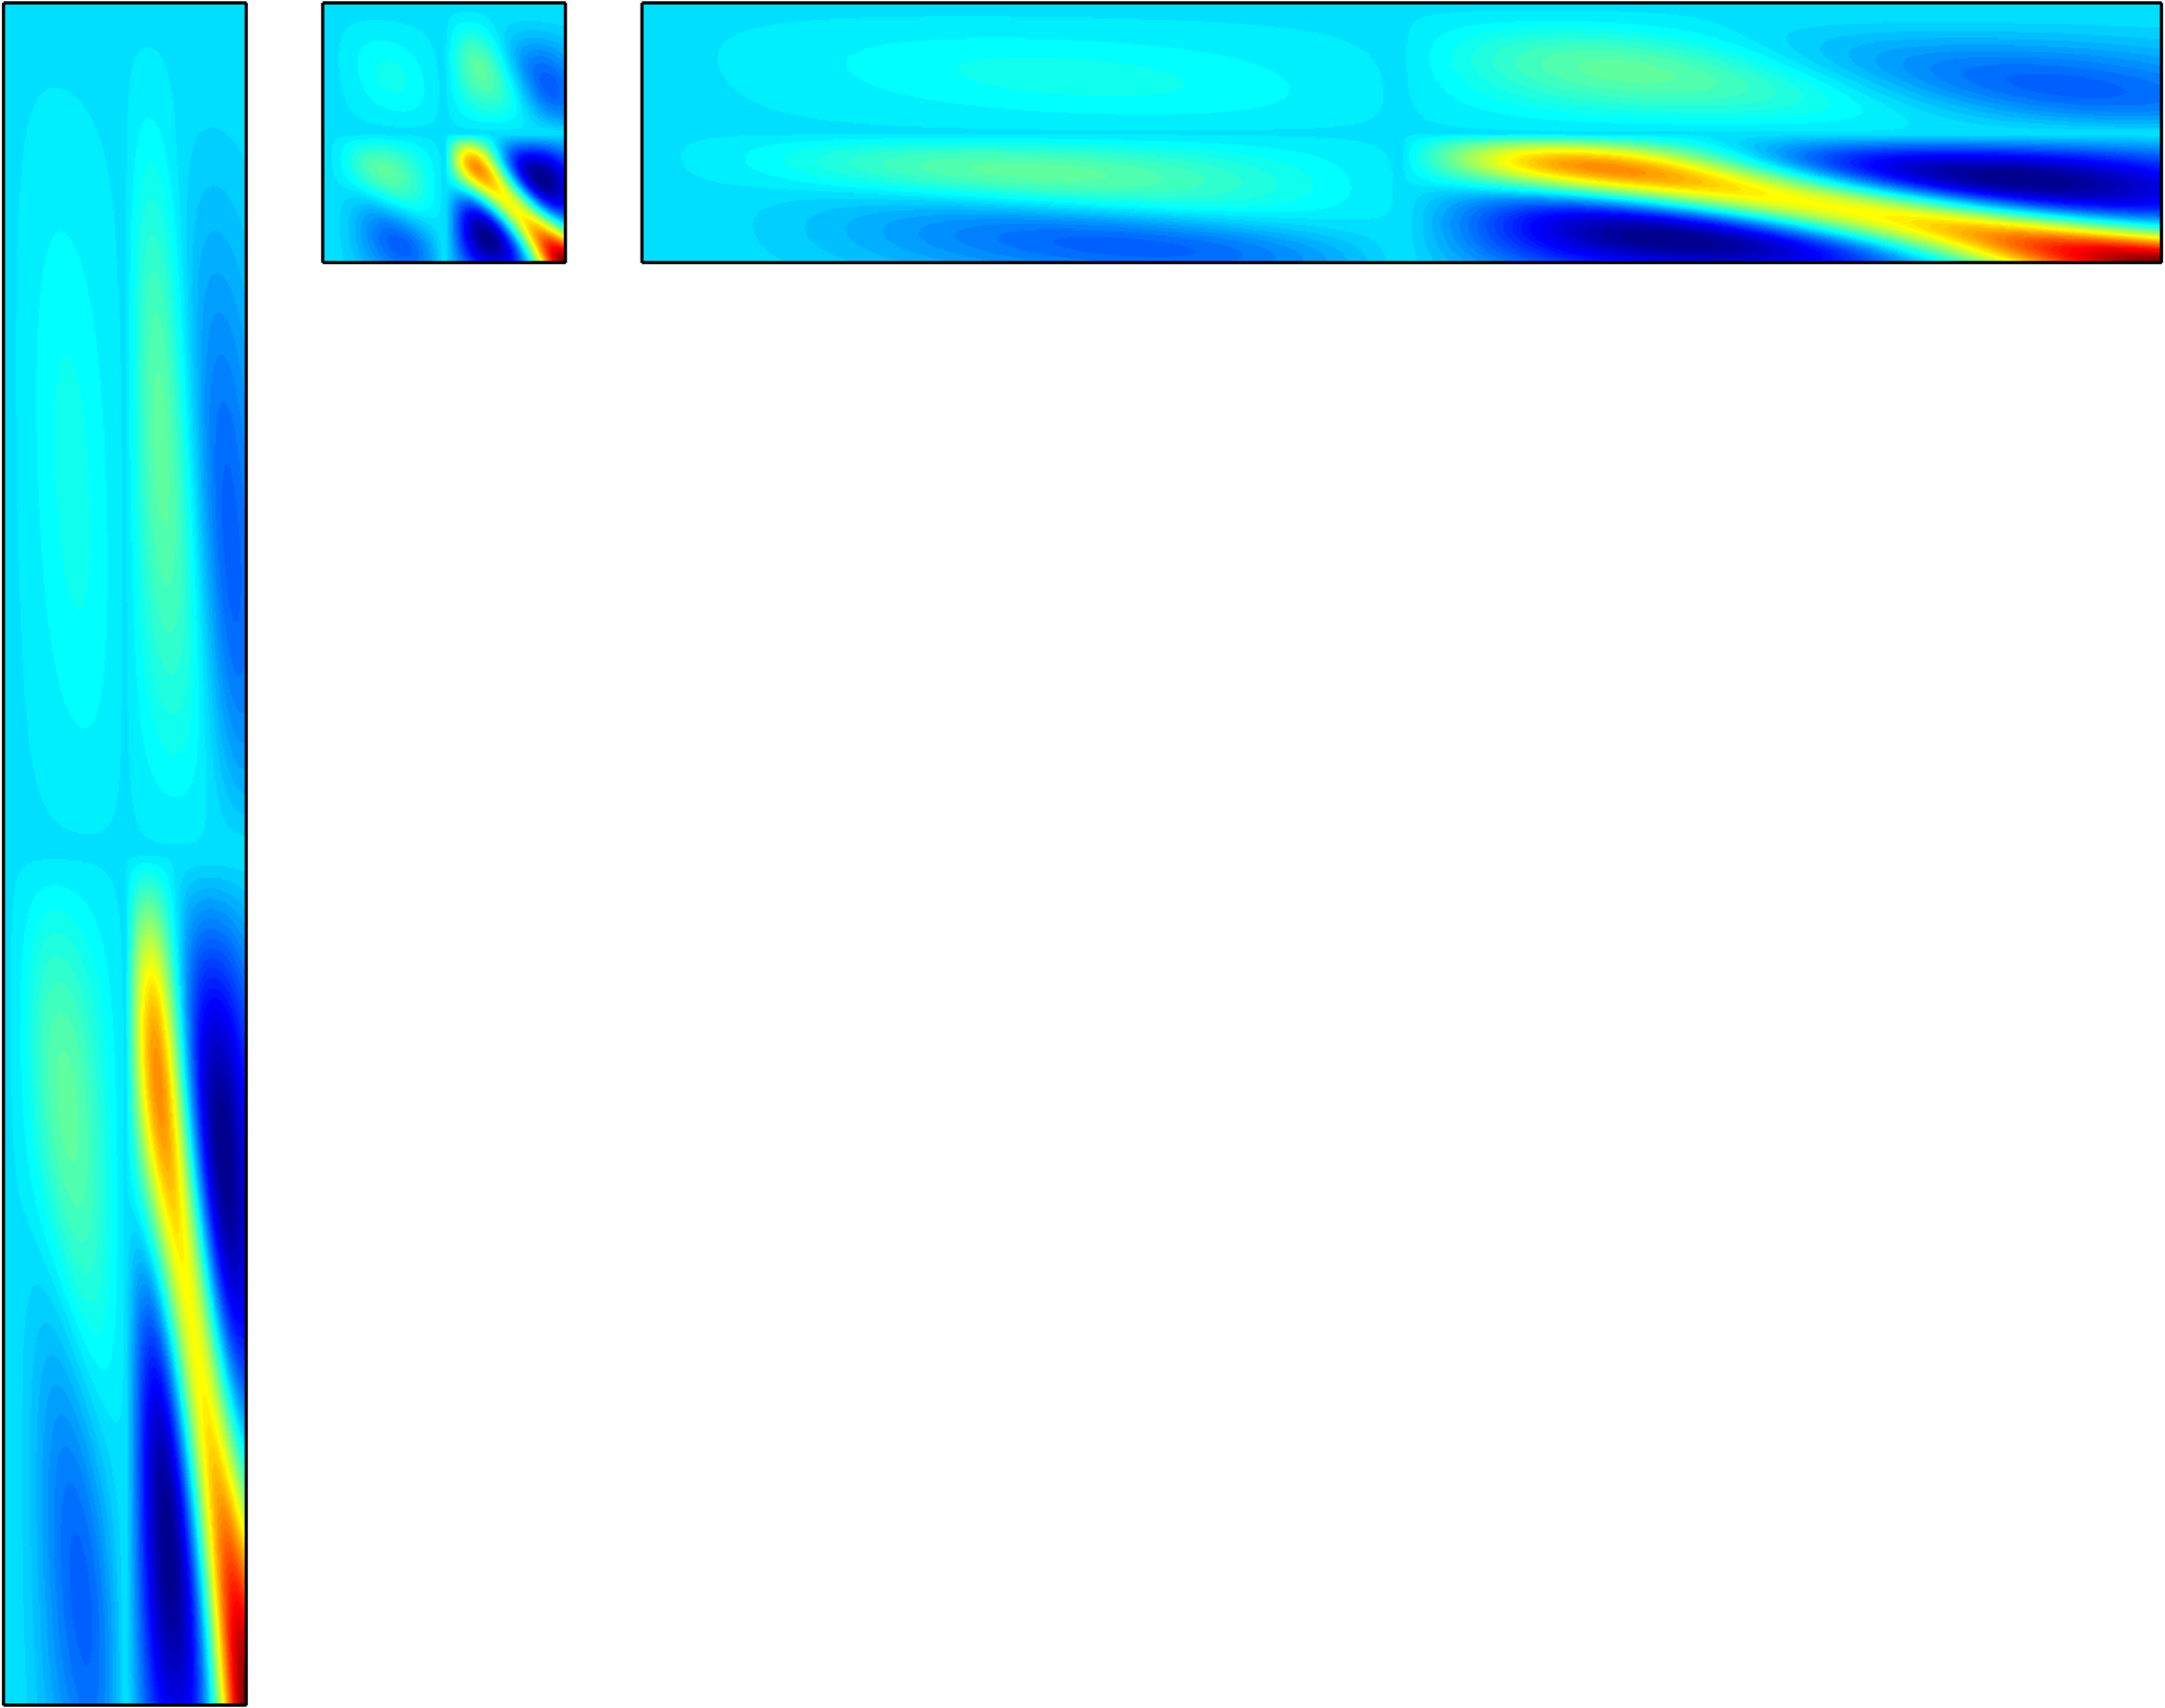
\includegraphics[width=0.45\textwidth]{images/kPredNystormMultipleOutputIntegral}\label{subfig:kPredNystormMultipleOutputIntegral}}
  \caption{Variational approximation of covariance matrix for Gaussian Process Regression}
\end{figure}


We try to approximate the joint-posterior distribution \(p(X| Y)\) by introducing a variational distribution \(q(X)\). In the case of varying number of inputs for different outputs, we place the inducing points over the input space and extend the derivation of \cite{Titsias09variationallearning} to multi-output case. 

\begin{equation}\label{eq:multiVariationalQ}
 q(X) = \mathcal{N}(X|  \mu, A)
\end{equation}
 
Here \(\mu\) and \(A\) are parameters of the variational distribution. We follow the derivation provided in \cite{Titsias09variationallearning} and obtain the lower bound of true marginal likelihood.

\begin{equation}\label{eq:lowerBoundMultiVarNLML}
F_{V} = log(\mathcal{N}[Y| 0, \sigma ^{2}I + Q_{XX}]) - \frac{1}{2\sigma ^{2}}Tr(\tilde{K})
\end{equation}

where \(Q_{XX} = K_{XX_{M}}K_{X_{M}X_{M}}^{-1}K_{X_{M}X}\) and \(\tilde{K} = K_{XX} - K_{XX_{M}}K_{X_{M}X_{M}}^{-1}K_{X_{M}X}\). \(K_{XX}\) is the joint-covariance matrix derived using equation \ref{eq:exactJointCovariance} using the input vector \(X\) defined in section \ref{sec:introduction}. \(K_{X_{M}X_{M}}\) is the joint-covariance function on the inducing points \(X_{M}\), such that \(X_{M} = [x_{M1}, x_{M2}, ..., x_{M2}]\). We assume that the inducing points \(x_{Mi}\) will be same for all the outputs, hence \(x_{M1} = x_{M2} = ... = x_{M2} = x_{M}\). While \(K_{XX_{M}}\) is the cross-covariance matrix between \(X\) and \(X_{M}\). 

Note that this bound consists of two parts. The first part is the log of a GP prior with the only difference that now the covariance matrix has a lower rank of \(MD\). This form allows the inversion of the covariance matrix to take place in \(\mathcal{O}\left ( N(MD)^{2} \right )\) time. The second part as discussed above can be seen as a penalization term that regularizes the estimation of the parameters. 

The bound can be maximized with respect to all parameters of the covariance function; both model hyperparameters and variational parameters. The optimization parameters are the inducing inputs \(x_{M}\), the hyperparameters \(\theta\) of the independent covariance matrix \(K_{22}\) and the error while measuring the outputs \(\sigma\). There is a trade-off between quality of the estimate and amount of time taken for the estimation process. On the one hand the number of inducing points determine the value of optimized negative log-marginal likelihood and hence the quality of the estimate. While, on the other hand there is a computational load of \(\mathcal{O}\left ( N(MD)^{2} \right )\) for inference. We increase the number of inducing points until the difference between two successive likelihoods is below a predefined quantity.   

\subsection{Distributed Inference on Multi-output GP}\label{sec:dMOGP}
An alternative to sparse approximations is to learn local experts on subset of data. Traditionally, each subset of data learns a different model from another, this is done to increase the expressiveness in the model \cite{rasmussen2002infinite}. The final predictions are then made by combining the predictions of local experts \cite{chen2009bagging}. 

An alternative way is to tie all the different experts using one single set of hyperparameters \cite{deisenroth2015distributed}. This is equivalent to assuming one single GP on the whole dataset such that there is no correlation across experts as seen in figure \ref{subfig:distributedFullKernelMatrix}. This tying of experts acts as a regularization and inhibits overfitting. Although ignoring correlation among experts is a strong assumption, it can be justified if the experts are chosen randomly and with enough overlap. 

\begin{figure}[!t]
  \centering
  \subfigure[Full multi-output covariance matrix for fig: \ref{subfig:drawsIntegralRelationship}]
  {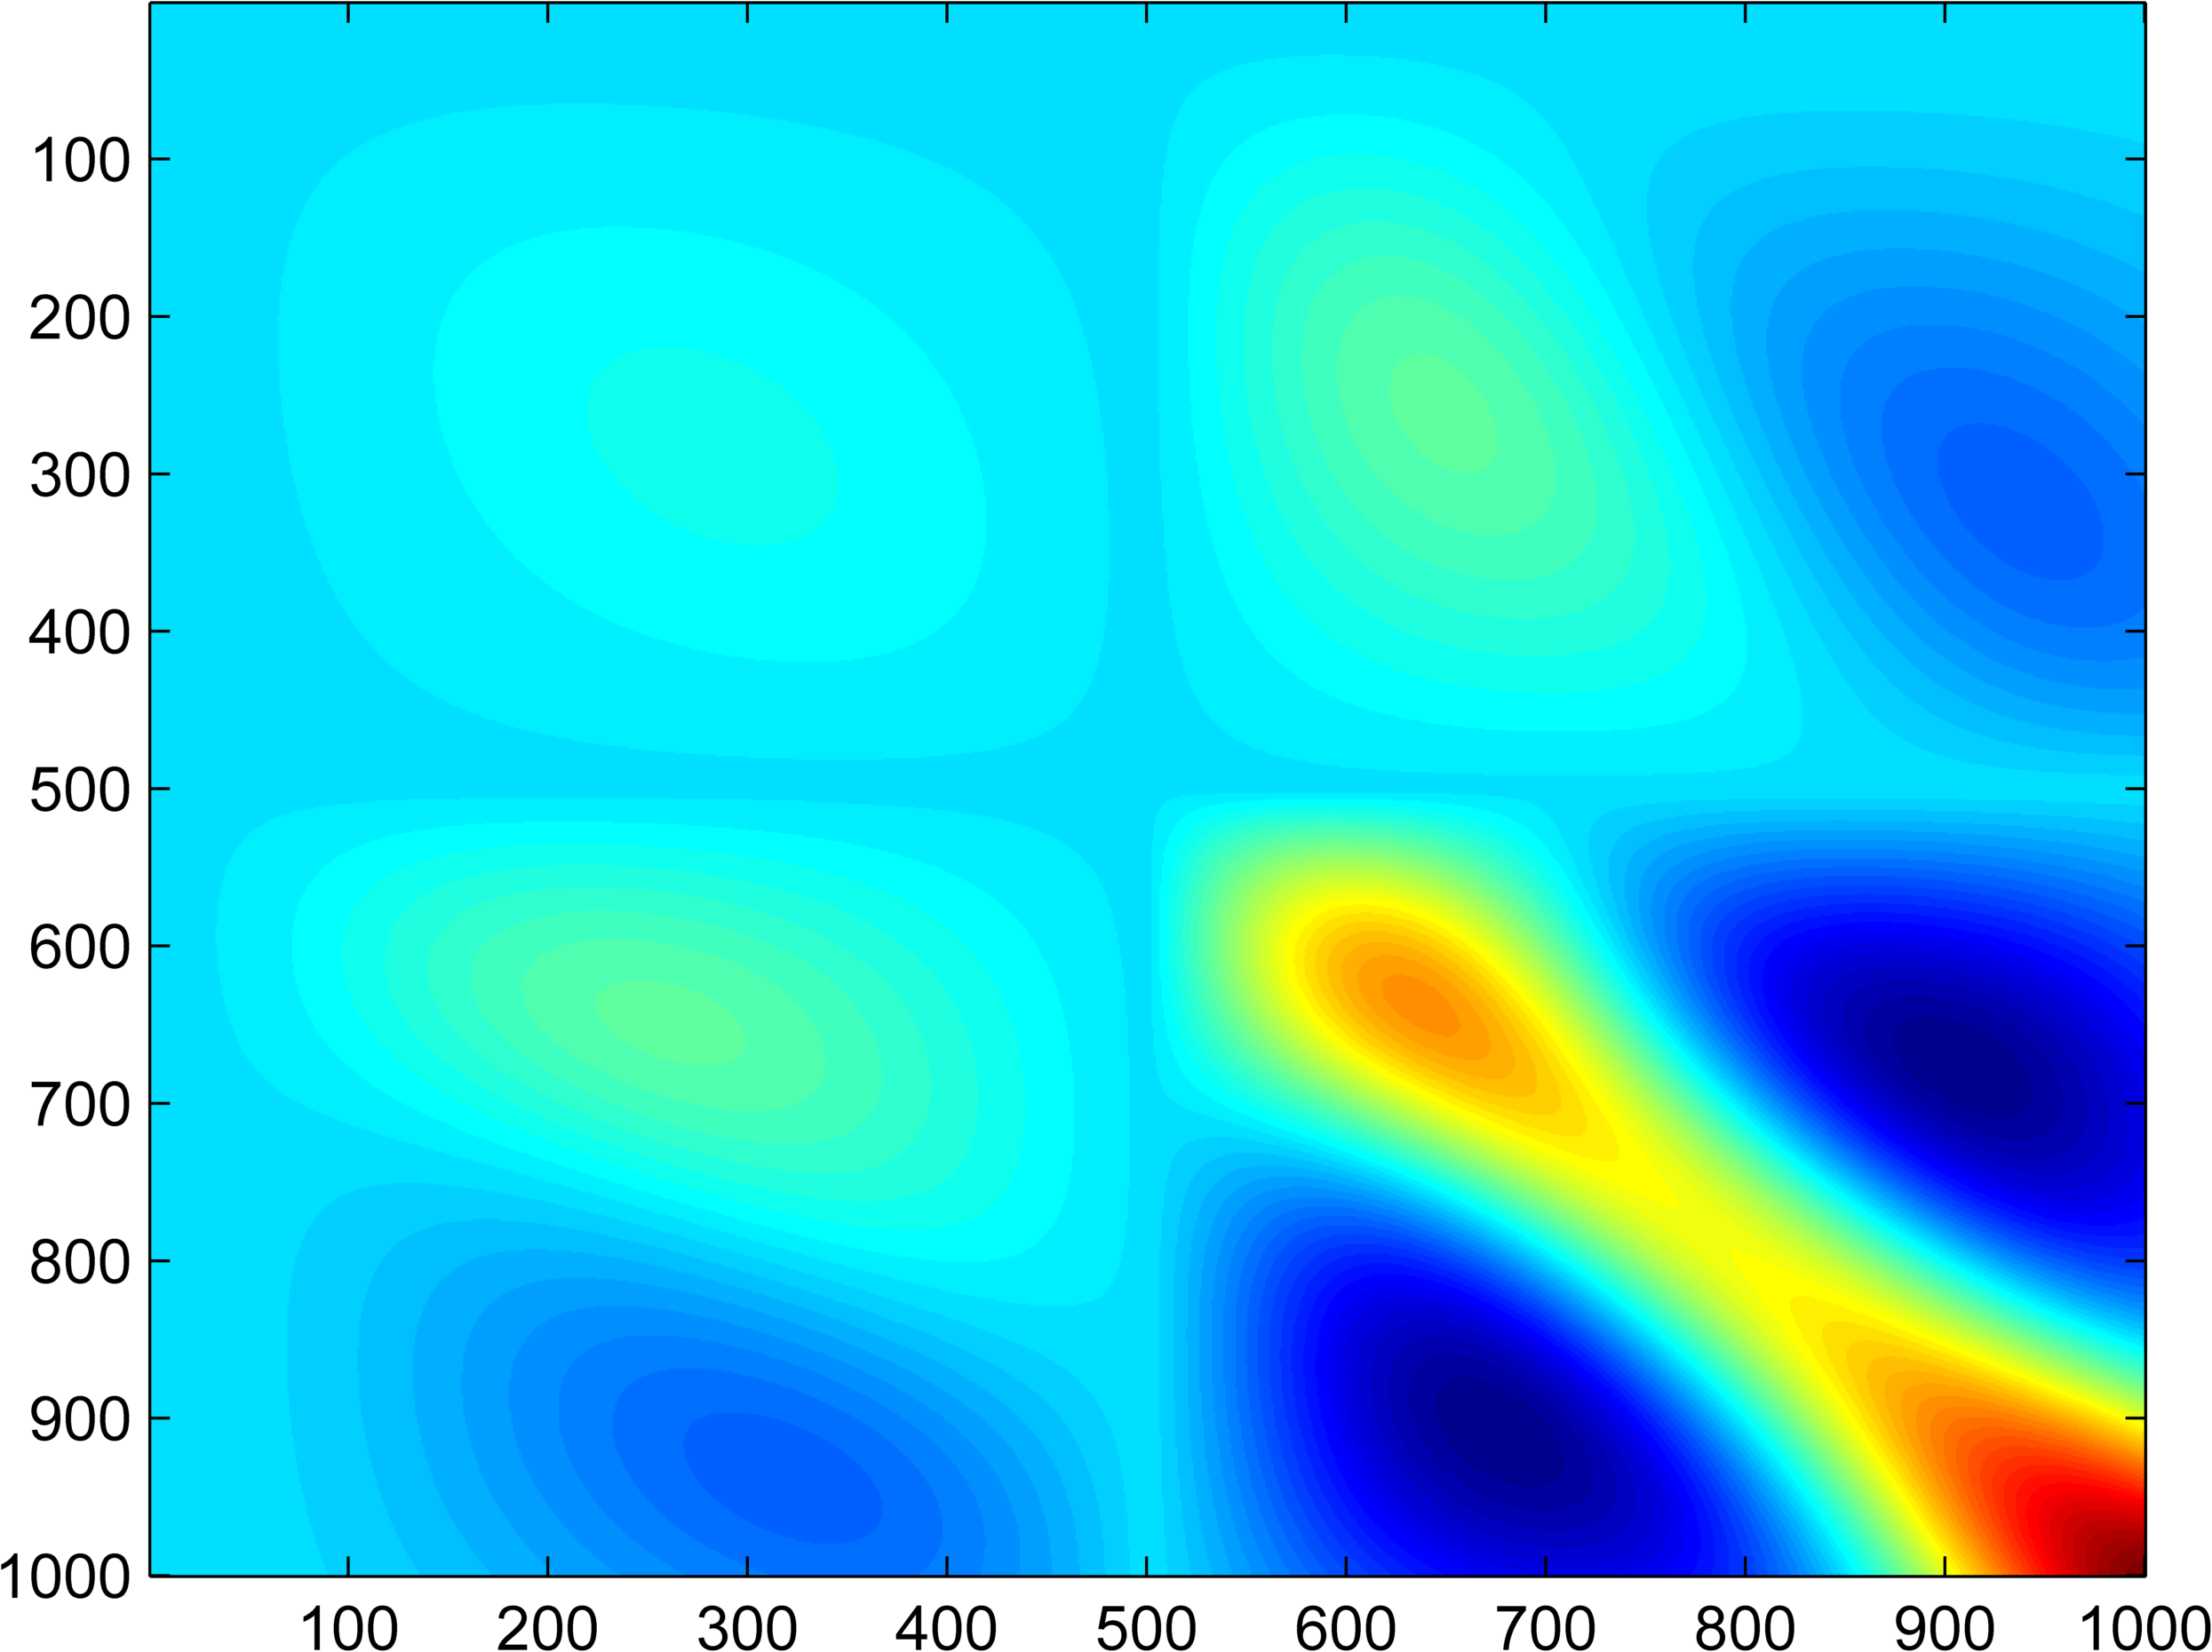
\includegraphics[width=0.45\textwidth]{images/kPredMultipleOutputIntegral}}\quad
  \subfigure[Distributed multi-output covariance matrix for fig: \ref{subfig:drawsIntegralRelationship} the cross-diagonal terms (blue) are zero due to independence between experts]
  {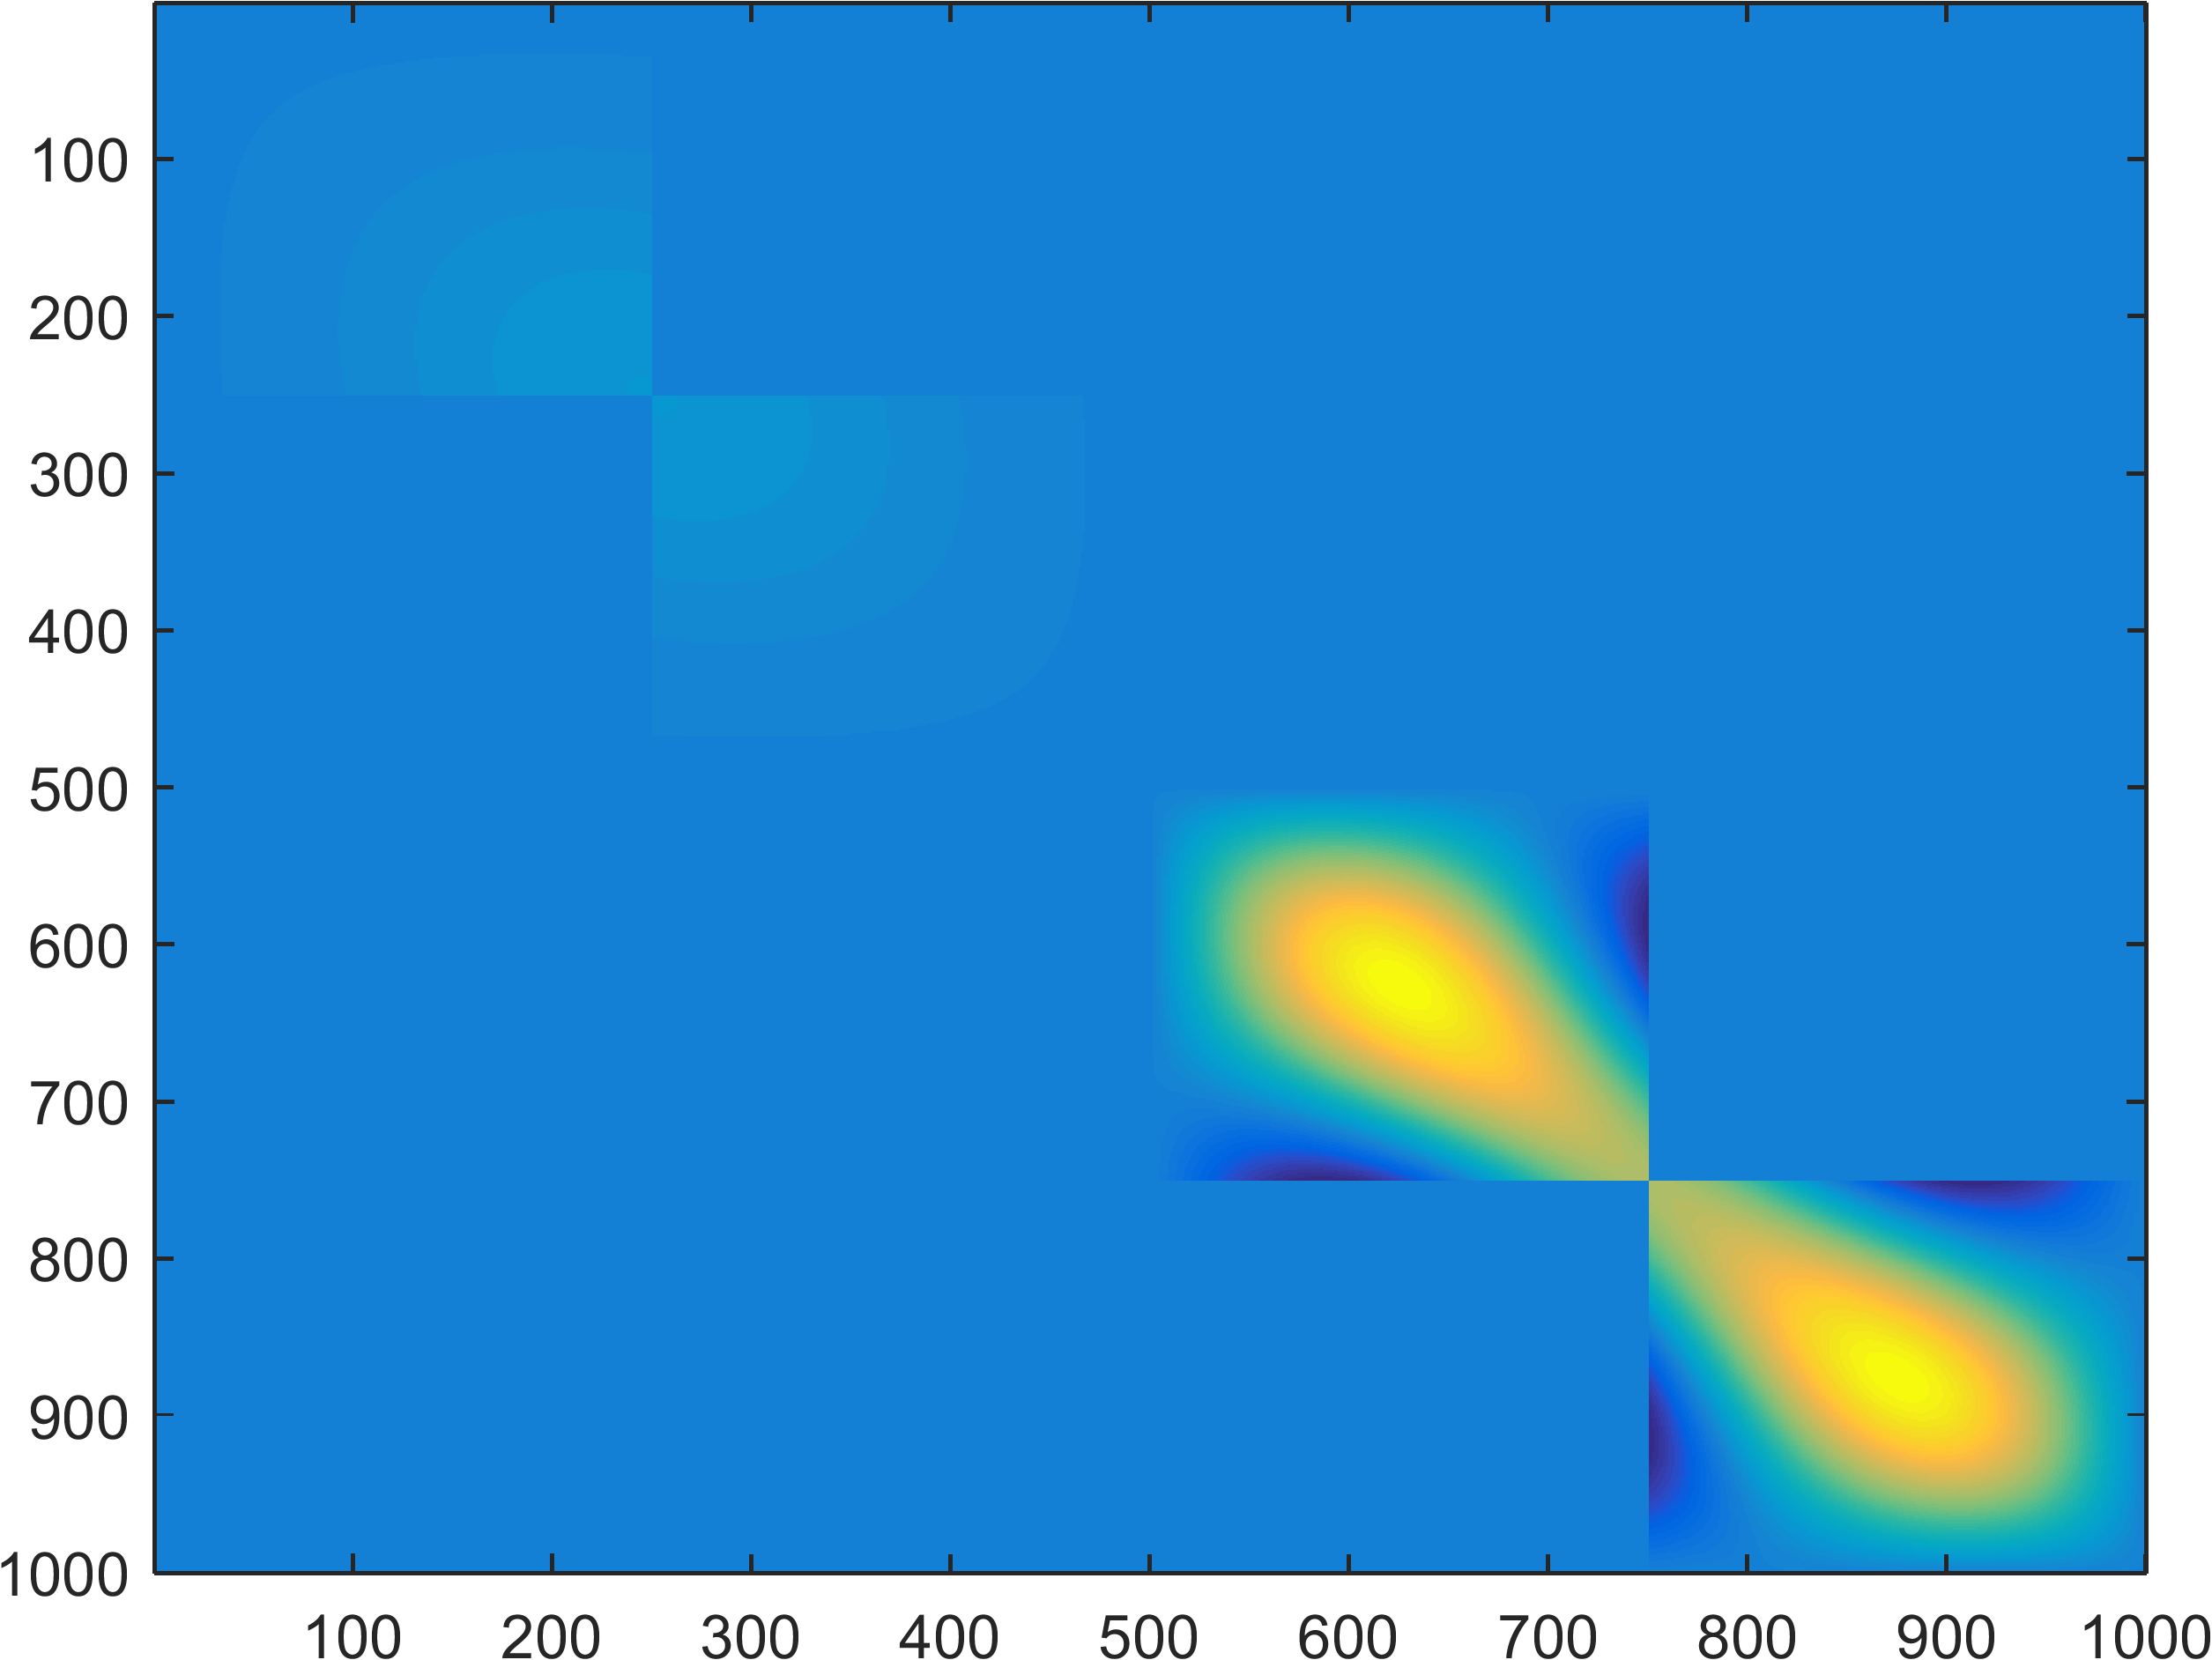
\includegraphics[width=0.45\textwidth]{images/distributedFullKernelMatrix}\label{subfig:distributedFullKernelMatrix}}
  \caption{Distributed approximation of covariance matrix for Gaussian Process Regression}
\end{figure}

If we partition the dataset into M subsets such as $\mathcal{D}^{(i)} = {X^{(i)}, y^{(i)}}, i = 1, \ldots M$. 

\begin{align}\label{eq:dGPNLML}
    \log p(y| X, \theta) \approx \sum_{k=1}^{M} \log p_{k}(y^{(i)}| X^{(i)}, \theta)
 \end{align}

The above equation \ref{eq:dGPNLML} describes the formulation for marginal likelihood. Due to the independence assumption the marginal likelihood can be written as a sum of individual likelihoods and then can be optimized to find the best-fit hyperparameters. After learning the hyperparameters we can combine the predictions of local experts to give mean and variance predictions. The robust Bayesian Commitee Machine (rBCM) model combines the various experts using their confidence on the prediction point \cite{deisenroth2015distributed}. In such manner experts which have high confidence at the prediction points get more weight when compared to experts with low confidence. 

\begin{equation}\label{eq:meanDGP}
    m(Y_{*}) = (Cov(X_{*}))^{-2}\sum \beta_{k}\sigma_{k}^{-2}m_{k}(X_{*})
\end{equation}

\begin{equation}
    (Cov_((Y_{*}))^{^-2} = \sum_{k} \beta_{k}\sigma_{k}^{-2} + (1- \sum_{k} \beta_{k})\sigma^{-2}_{**}
\end{equation}

In the above equations \(m_{k}(X_{*})\) and \(\sigma_{k}\) are the mean and covariance predictions from expert \(k\) at point \(X_{*}\). \(\sigma_{**}\) is the auto-covariance of the prior at prediction points \(X_{*}\). \(\beta_{k}\) determines the influence of experts on the final predictions \cite{DBLP:journals/corr/CaoF14} and is given as \(\beta_{k} = \frac{1}{2}(\log\sigma_{**}^{-2} - \log\sigma_{k}^{-2})\).  

\section{Experiments}\label{sec:experiments}
\noindent We empirically assess the performance of distributed Gaussian Process and Variational Inference with respect to the training time and accuracy. We start with a synthetic dataset where we try to learn the model over derivative relationship and compare the two inference techniques. We then evaluate the improvement on real world flight-test dataset.

The basic toolbox used for this paper is GPML provided with \cite{Rasmussen2005}, we generate covariance functions to handle relationships as described in equations \ref{eq:exactJointCovariance} using the ``Symbolic Math Toolbox" in MATLAB 2014b. Variational inference is wrapped from gpStuff toolbox \cite{Vanhatalo:2013:GBM:2567709.2502617} and distributed GP is inspired from \cite{deisenroth2015distributed}. All experiments were performed on an Intel quad-core processor with 4Gb RAM.
  
\subsection{Experiments on Theoretical Data}\label{sub:experimentsSyntheticData}
We consider a derivative relationship between two output functions as described in equation \ref{eq:physicalRelation}. Such that 

\begin{equation*}\label{eq:derivativeEquation}
   g(f, x) = \frac{\partial f}{\partial x} 
\end{equation*}

Since the differential relationship \(g(.)\) is linear in nature we use the equation \ref{eq:exactJointCovariance} to calculate the auto- and cross-covariance functions as shown in table \ref{tab:differentialCovariances}.

\begin{table}[h]
\renewcommand{\arraystretch}{1.5}
\caption{Auto- and cross-covariance functions for a differential relationship.}\label{tab:differentialCovariances} \centering
\begin{tabular}{|c|c|c|}
  \hline
  Initial Covariance & \(K_{22}\) & \(\sigma ^{2}exp(\frac{-1}{2}\frac{d^{2}}{l^{2}})\) \\
  \hline
  Cross-Covariance & \(K_{12}\) &  \(\sigma ^{2}\frac{d}{l^{2}}exp(\frac{-1}{2}\frac{d^{2}}{l^{2}})\) \\
  \hline
  Auto-covariance & \(K_{11}\) & \(\sigma ^{2}\frac{d^{2}-l^{2}}{l^{4}}exp(\frac{-1}{2}\frac{d^{2}}{l^{2}})\) \\
  \hline
\end{tabular}
\end{table}

Data is generated from equations \ref{eq:experimentalSET}, a random function is drawn from GP to get \(f_{2}\) whose derivative is then calculated to generate \(f_{1}\). \(y_{1}\) and \(y_{2}\) are then calculated by adding noise according the the equations \ref{eq:experimentalSET}. 10,000 points are generated for both the outputs \(y_{1}\) and \(y_{2}\). Values of \(y_{2}\) are masked in the region \(x \in [0, 0.3]\) the remaining points now constitute our training dataset. 

\begin{equation*}
f_{2} \sim  GP[0, K_{SE}(0.1, 1)]
\end{equation*}
\begin{equation*}
\sigma_{n2} \sim \mathcal{N}[0, 0.2]
\end{equation*}
\begin{equation}\label{eq:experimentalSET}
\sigma_{n1} \sim \mathcal{N}[0, 2]
\end{equation}

\(K_{SE}(0.1, 1)\) means squared exponential kernel with length scale 0.1 and variance as 1.

\begin{figure*}[!ht]
  \centering
  \subfigure[Independent fit for two GP's mean is represented by solid black line. 2\(\Sigma\) confidence band is represented by light red for \(f_{1}\) and light blue for \(f_{2}\).The dashed black line represents the true latent function values; noisy data is denoted by blue dots. Experiment was run on 10,000 points but only 100 data points are plotted to increase readibility. Inference is performed using variational inference algorithm and equidistant 100 inducing points. We can observe the huge difference between the real data and the predicted mean values at zone with no data.]
  {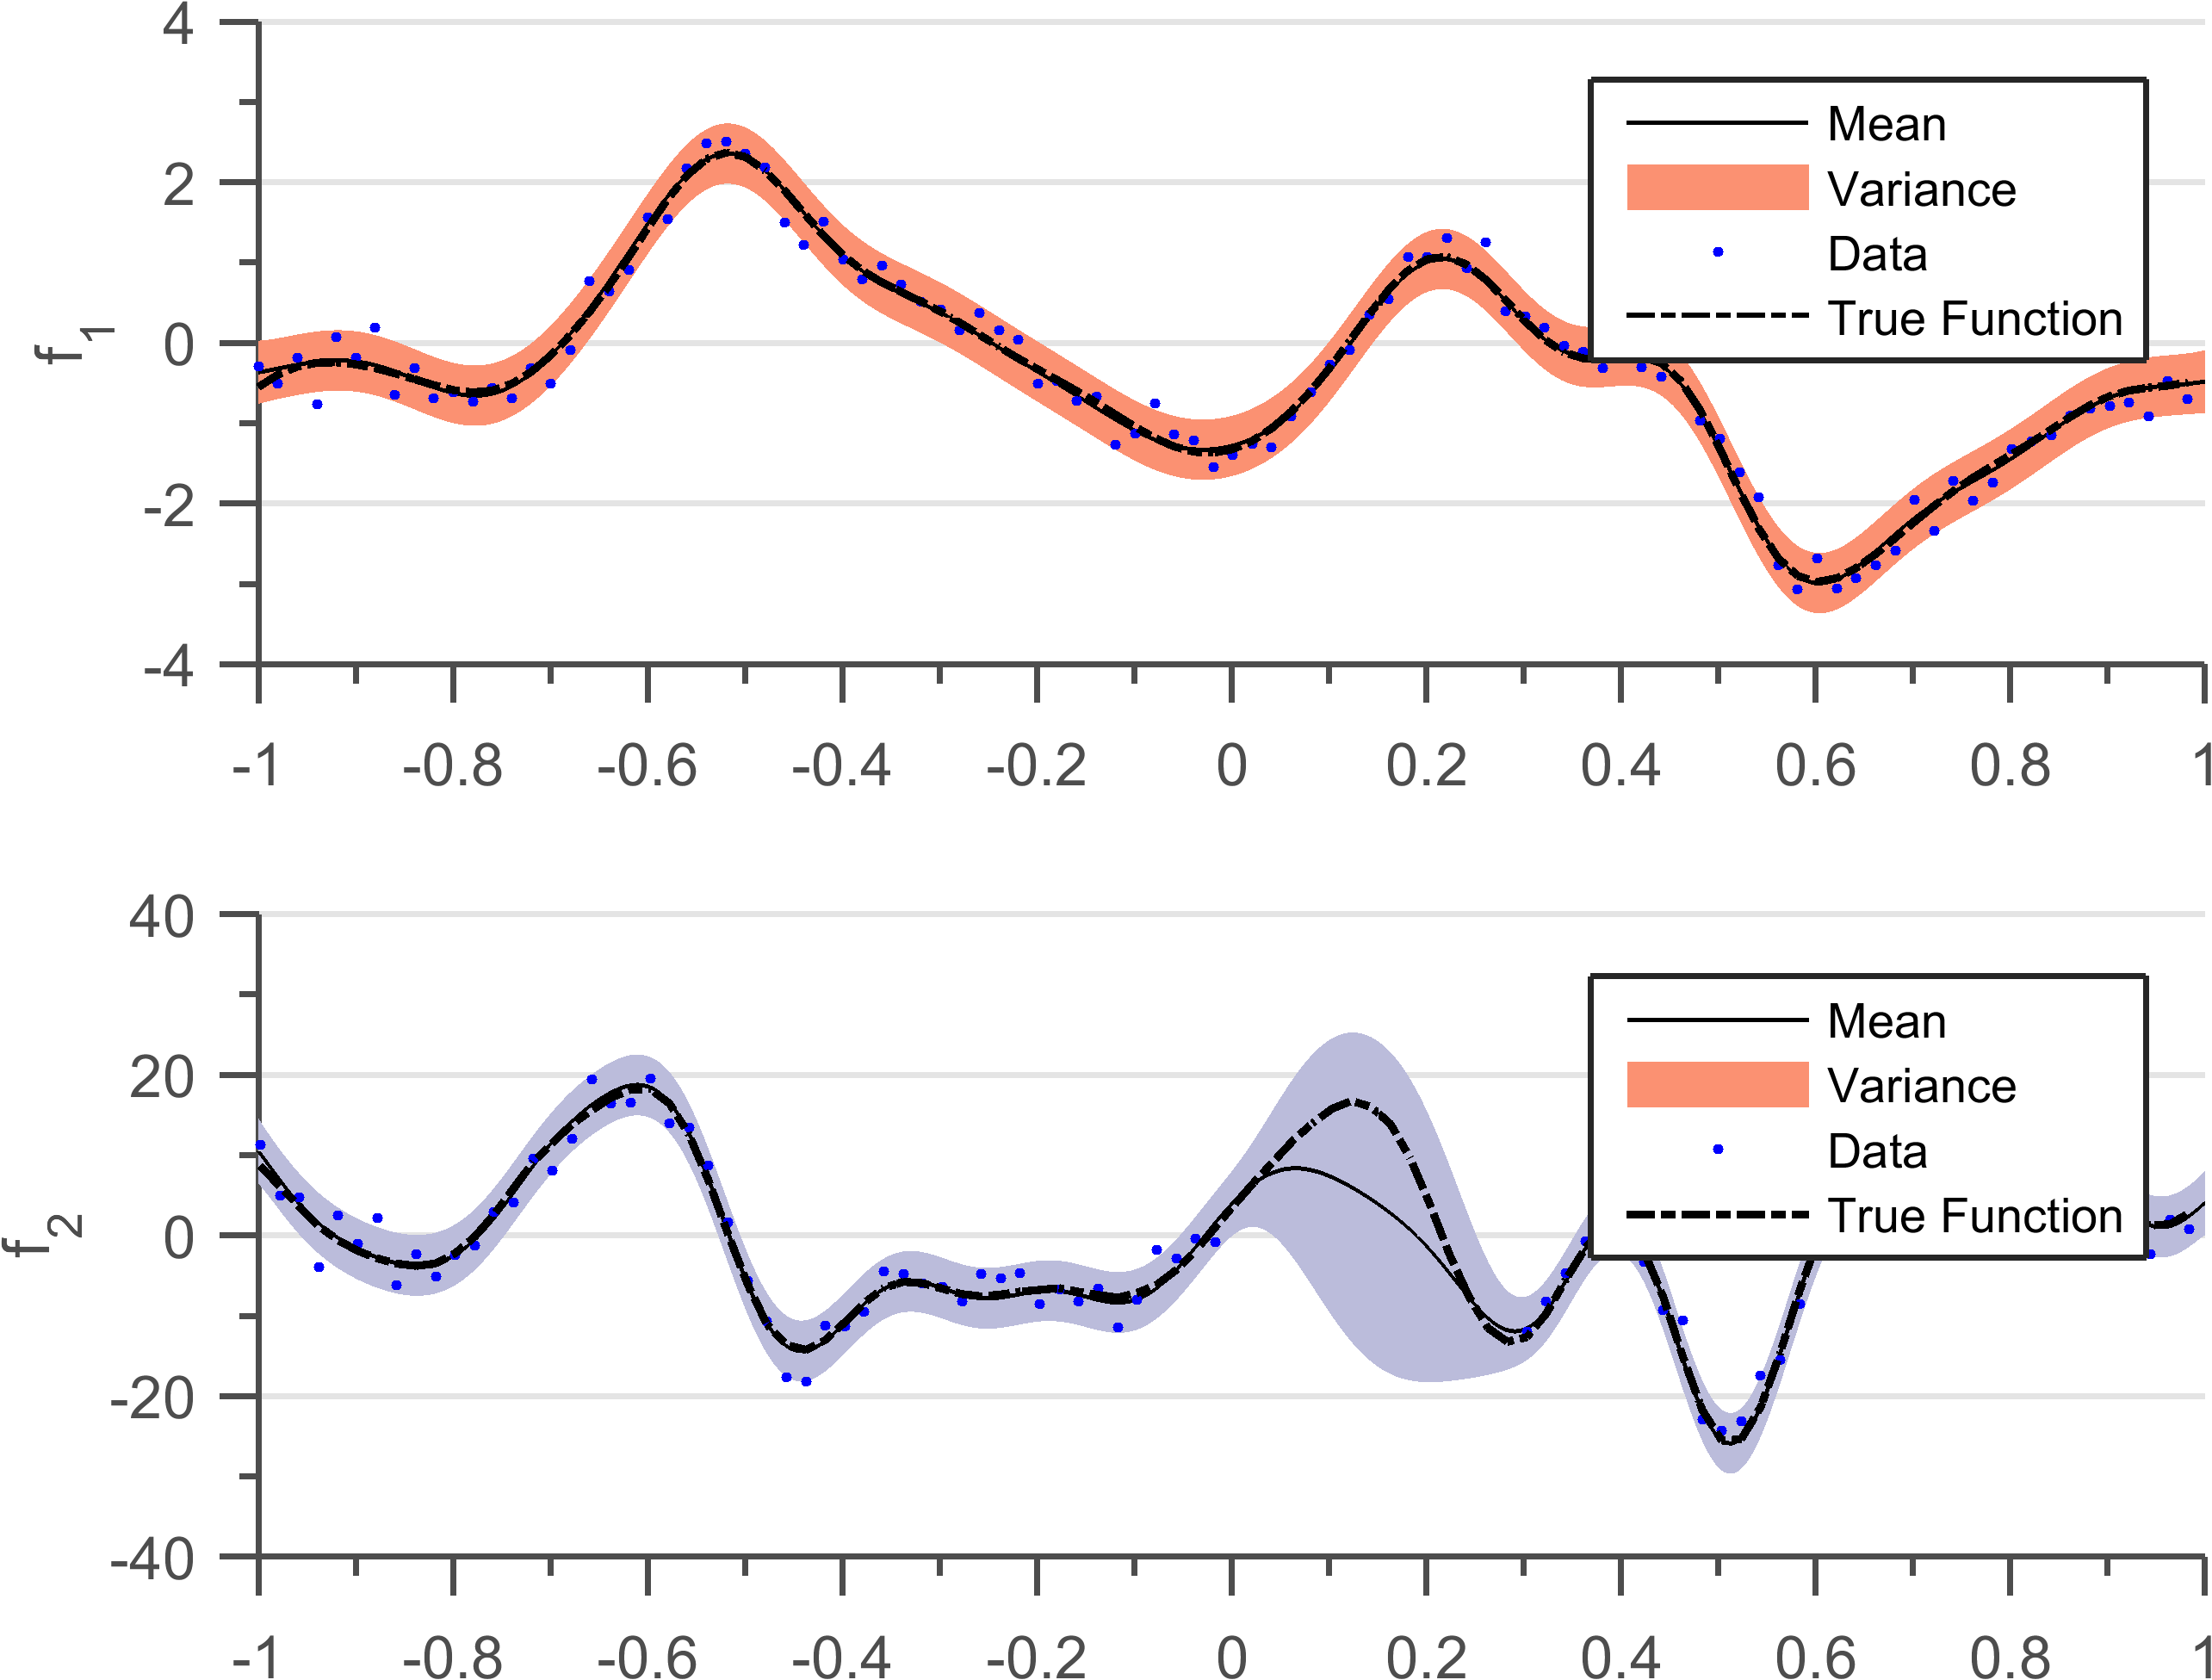
\includegraphics[width=0.48\textwidth]{images/independentFitRelatedGP}\label{subfig:independentFitRelatedGP}}\quad
  \subfigure[Joint multi-output GP's for two outputs, mean is represented by solid black line. 2\(\Sigma\) confidence band is represented by light red for \(f_{1}\) and light blue for \(f_{2}\).The dashed black line represents the true latent function values; noisy data is denoted by blue dots. Experiment was run on 10,000 points but only 100 data points are plotted to increase readibility. Inference is performed using variational inference algorithm and equidistant 100 inducing points. We can observe the improved prediction between zone with no data because information is being shared between the two outputs.]
  {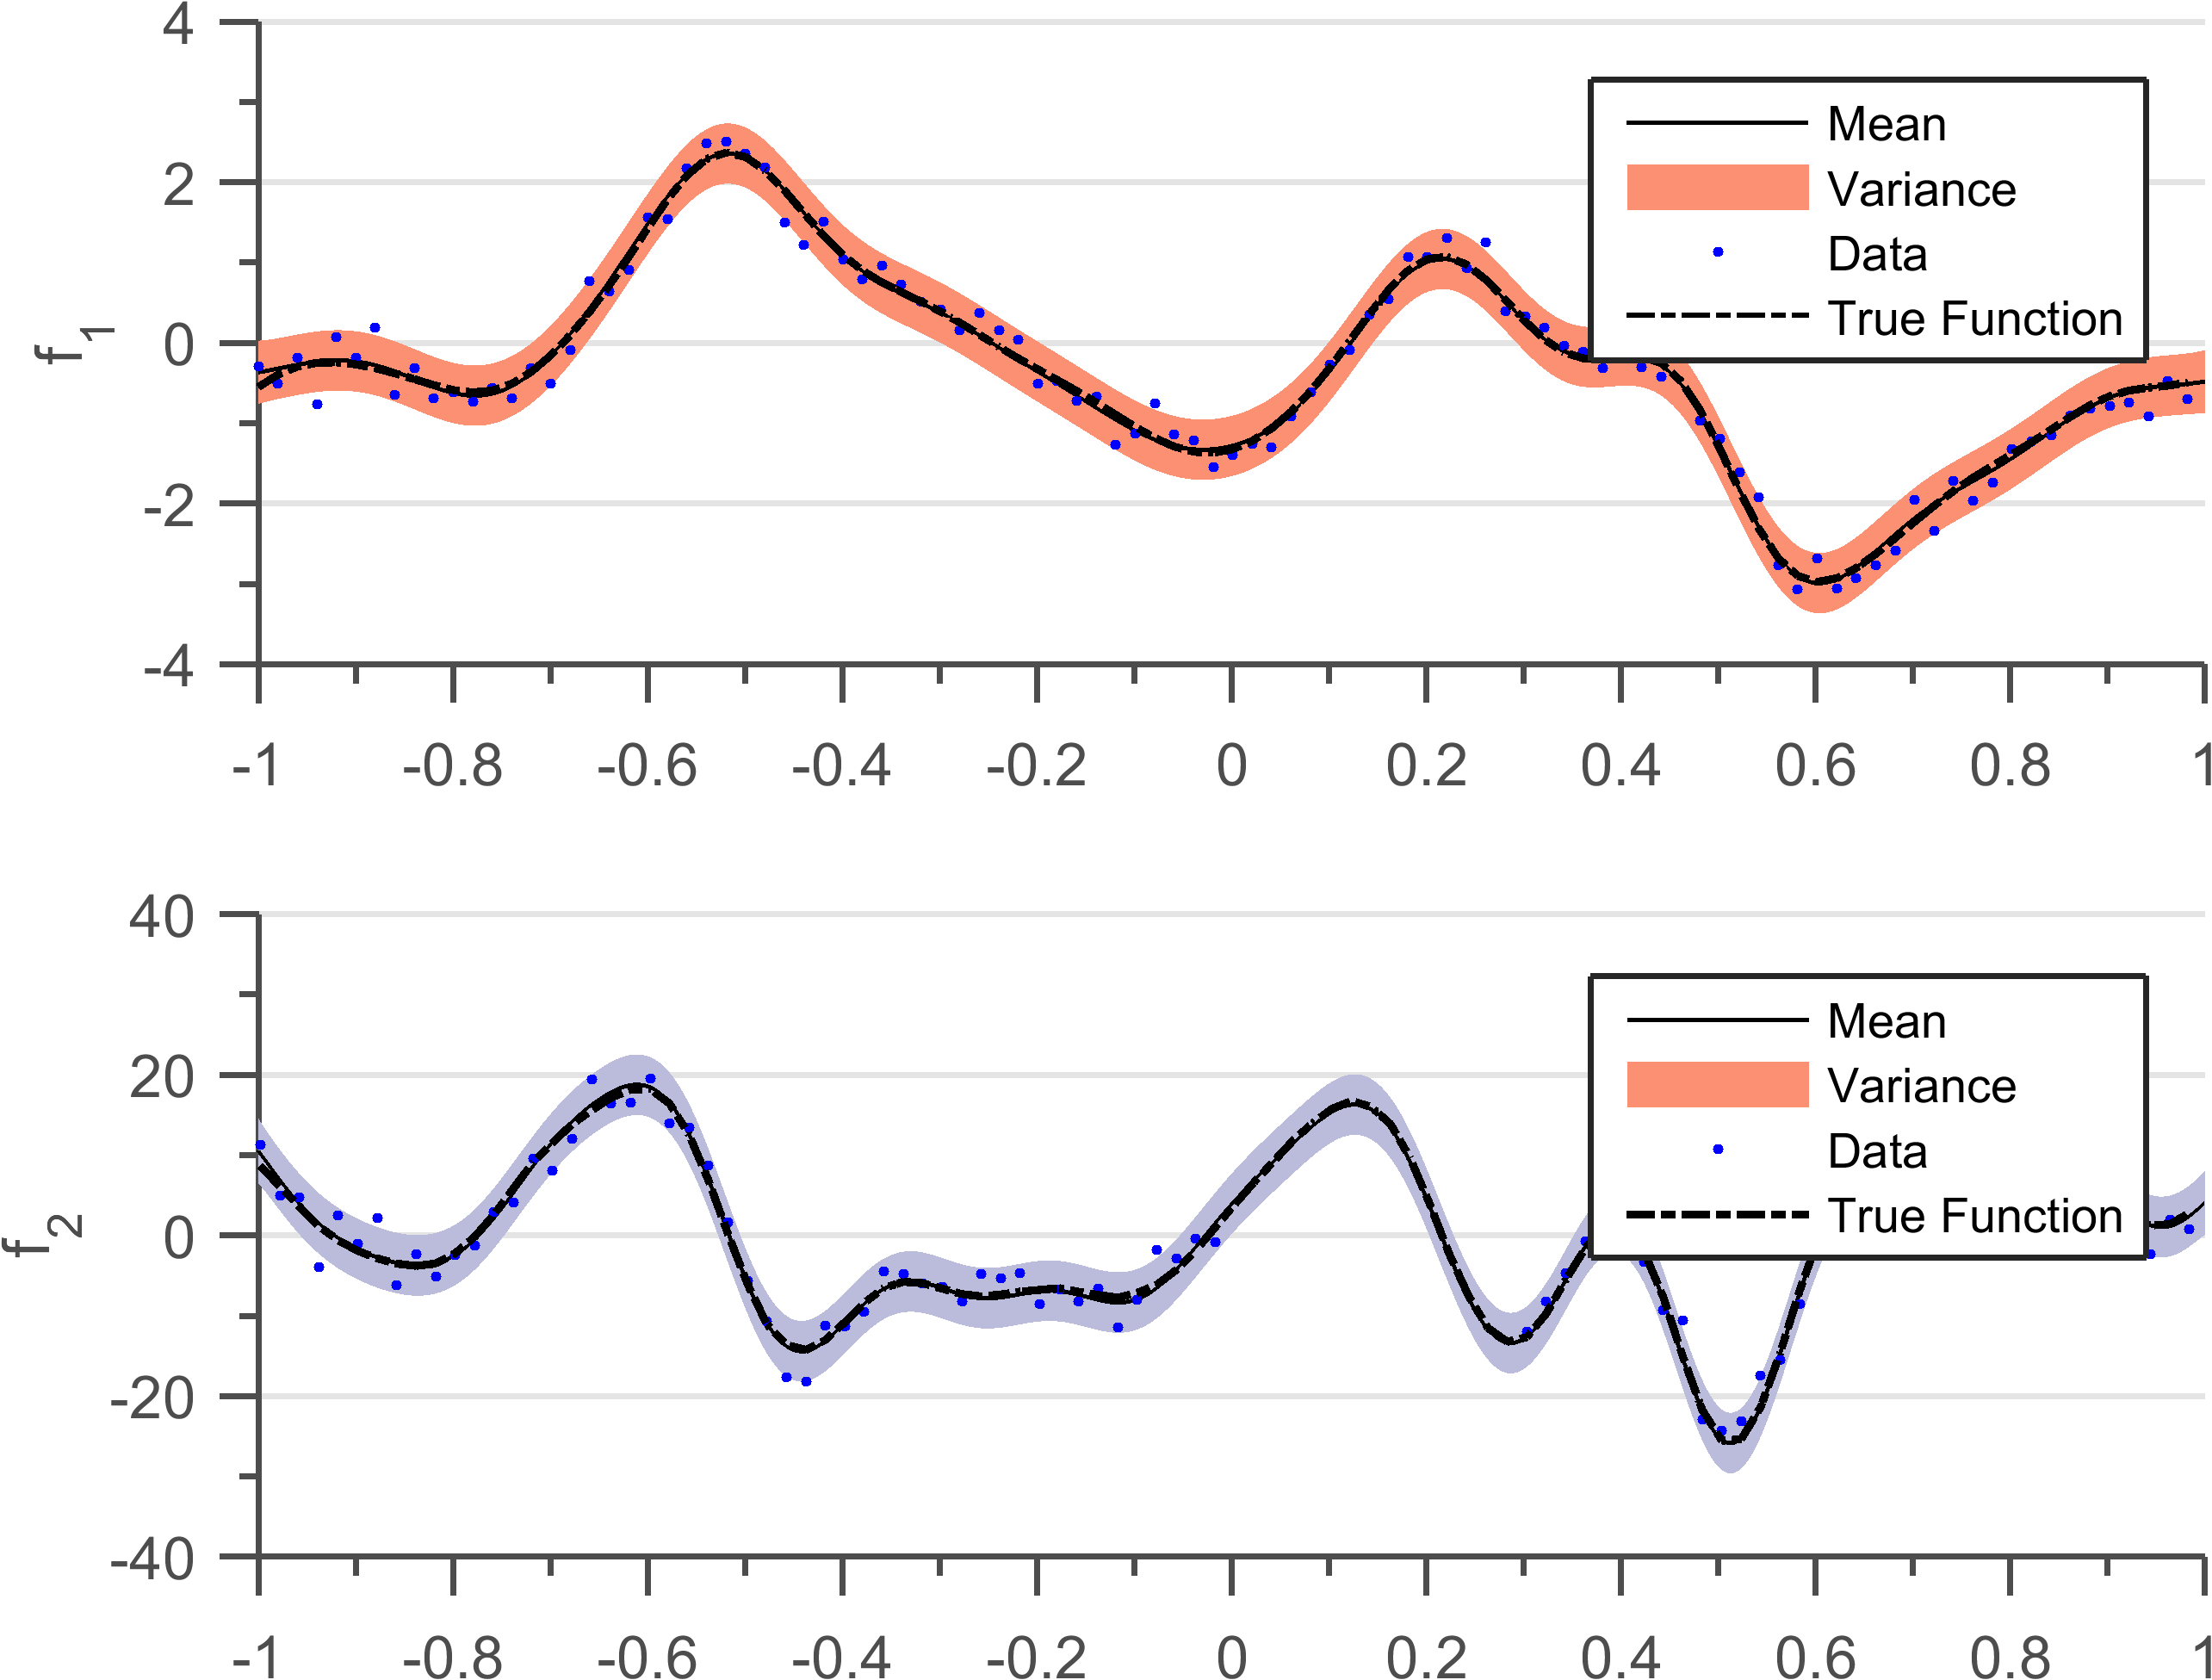
\includegraphics[width=0.48\textwidth]{images/dependentFitRelatedGP}\label{subfig:dependentFitRelatedGP}}
  \caption{Experimental results for differential relationship while using variational approximation}\label{fig:derivativeGP}
\end{figure*}

Figure \ref{fig:derivativeGP} shows comparison between an independent fit GP and a joint multi-output GP whose outputs are related through a derivative relationship described in equation \ref{eq:derivativeEquation}. For figure \ref{subfig:independentFitRelatedGP} using variational inference algorithm we optimize the lower bound of log-marginal likelihood, for independent GP's on \(y_{1}\) and \(y_{2}\). For figure \ref{subfig:dependentFitRelatedGP} using variational inference we optimize the same lower bound but with a joint-covariance approach as described in section \ref{sec:varMOGP} using \(y_{1}\), \(y_{2}\) and \(g(.)\). We settled on using 100 equidistant inducing points for this exercise \cite{icpram16Ankit} and have only optimized the hyperparameters to learn the model. 

Figure \ref{subfig:independentFitRelatedGP} shows the independent fit of two GP for the differential relationship, while figure \ref{subfig:dependentFitRelatedGP} shows the joint GP fit. The GP model with joint-covariance gives better prediction even in absence of data of \(y_{2}\) for \(x \in [0, 0.3]\).

\begin{figure*}[!ht]
  \centering
  \subfigure[Comparison of time to calculate negative log marginal likelihood for a Full GP, Variational inference and Distributed GP with increasing number of datapoints. We observe for datapoints greater that 10e5 the distributed GP algorithm starts outperforming variational inference]
  {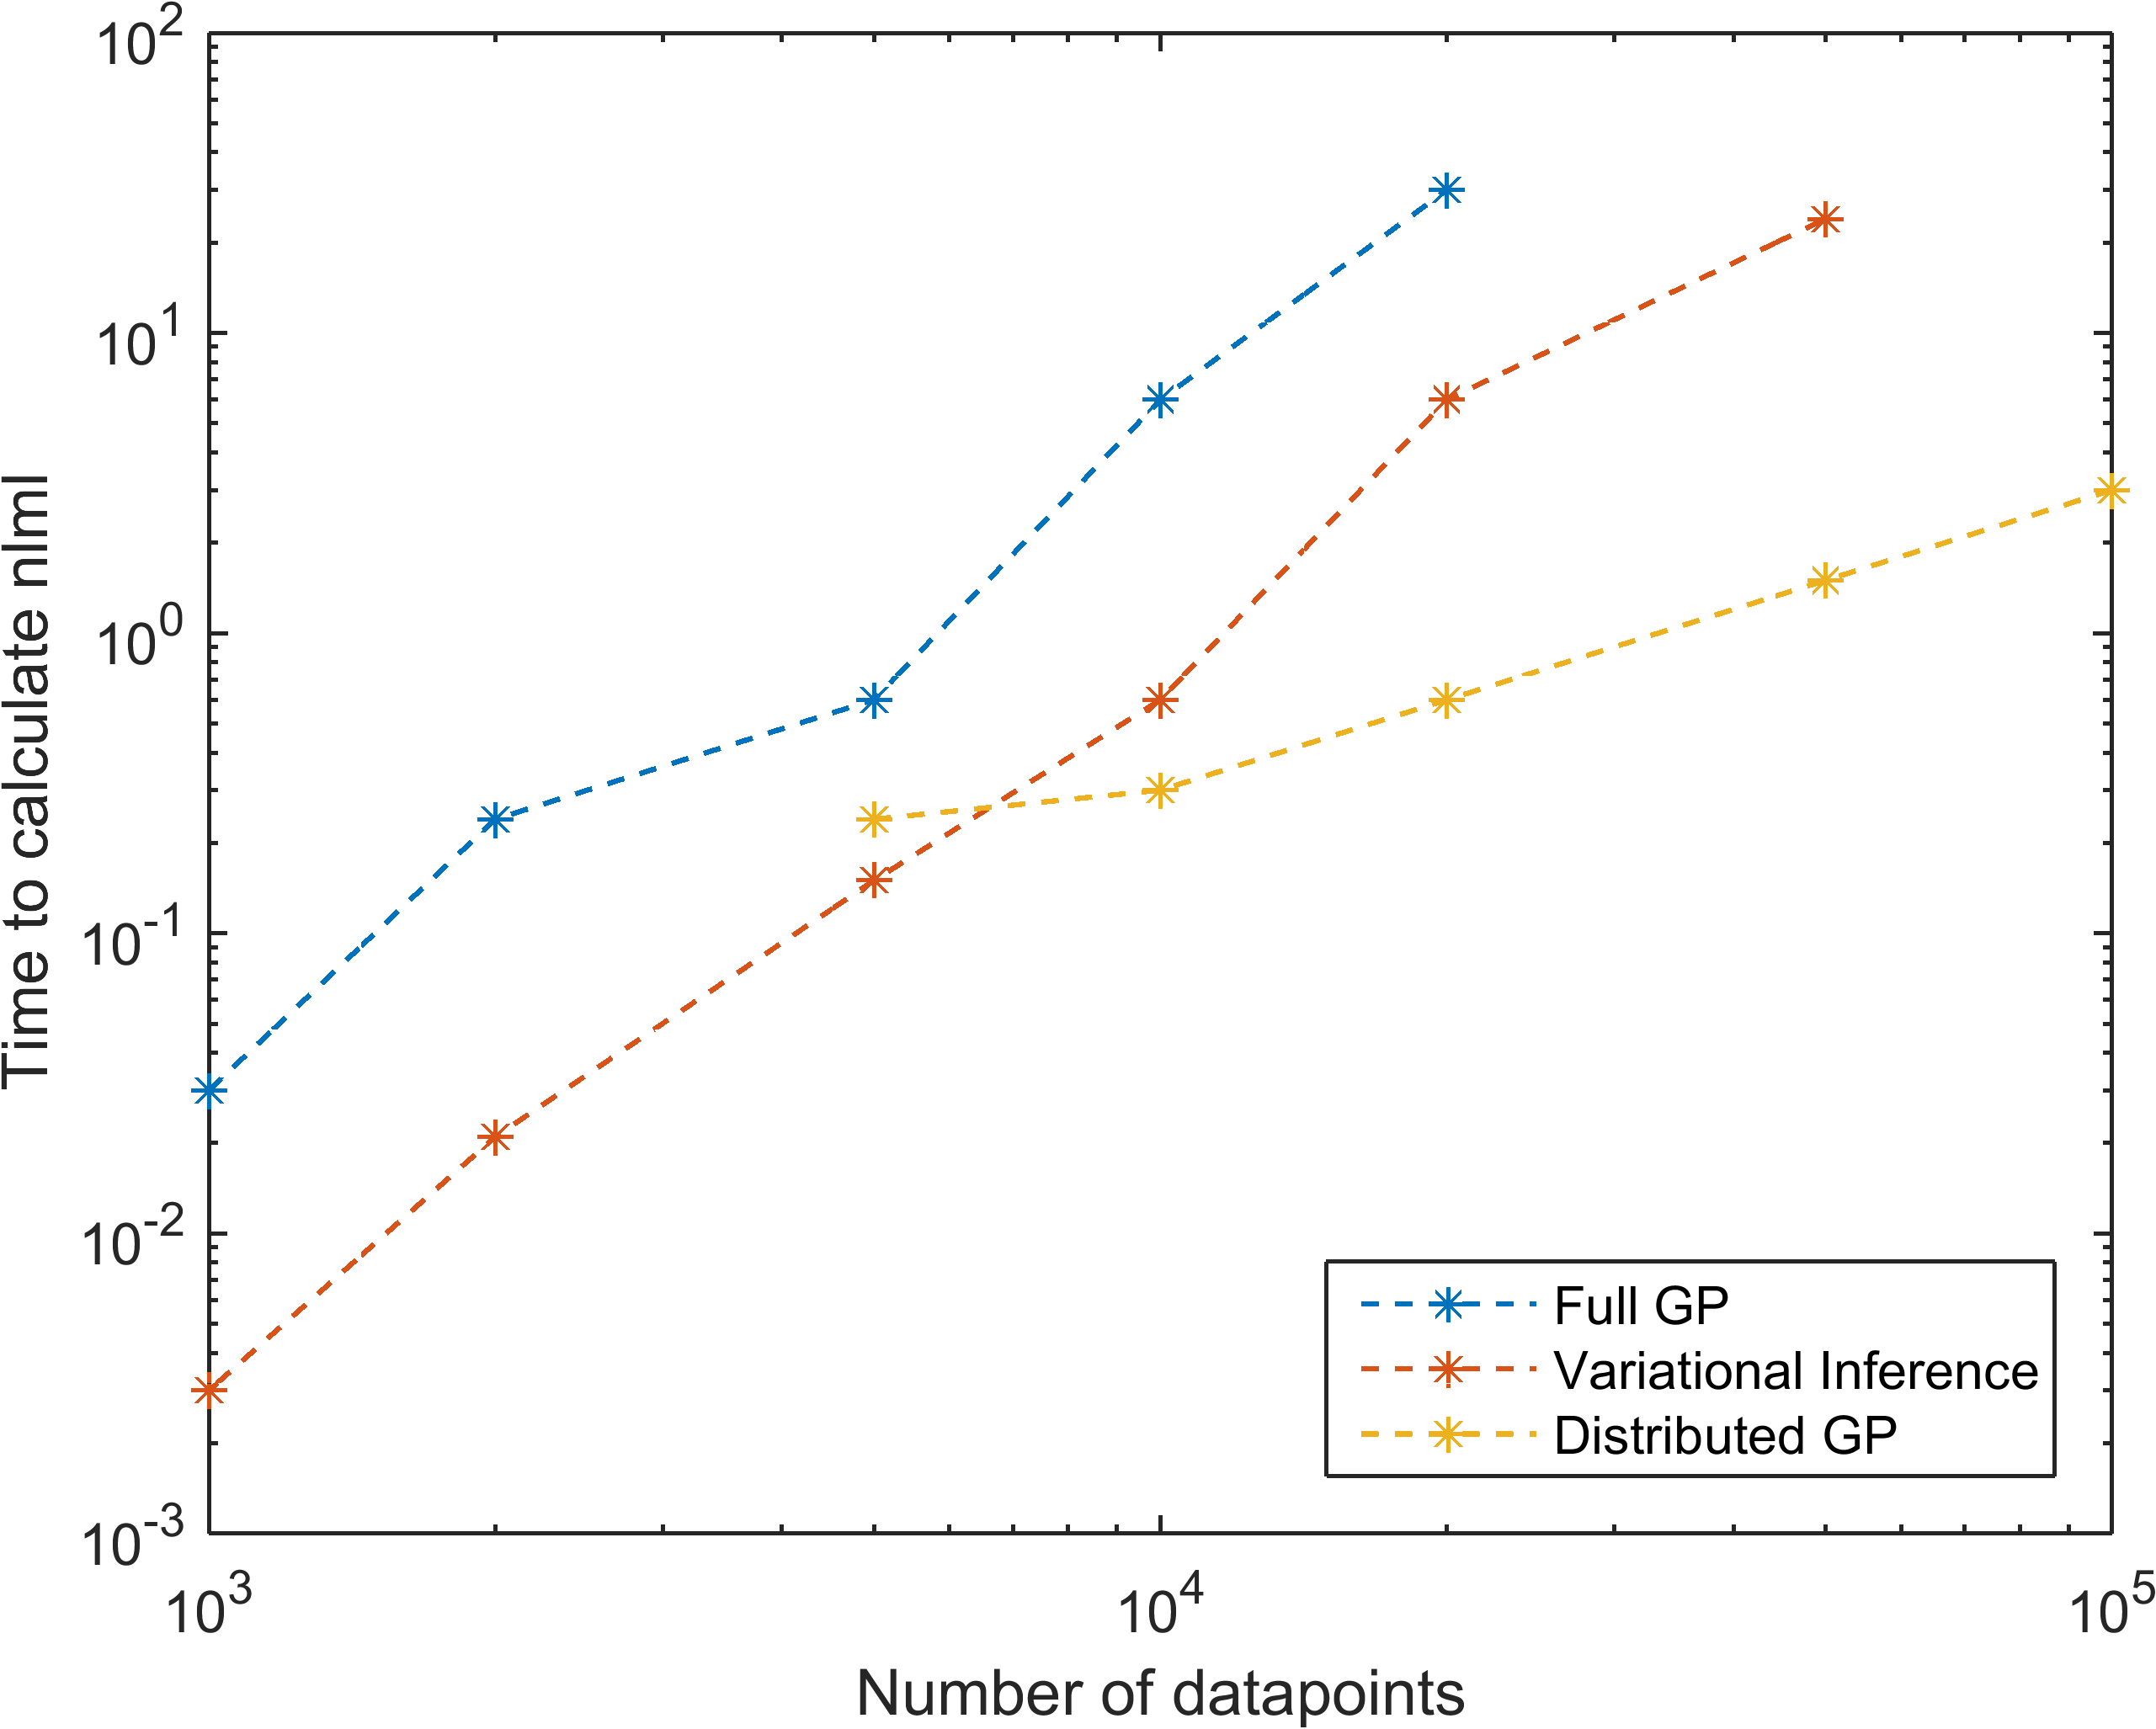
\includegraphics[width=0.48\textwidth]{images/comparisonOfRunTimes}\label{subfig:comparisonOfRunTimes}}\quad
  
  \subfigure[Comparison of RMSE for variational inference and distributed GP algorithm. We observe for datapoints greater that 10e4 the distributed GP algorithm starts outperforming variational inference.]
  {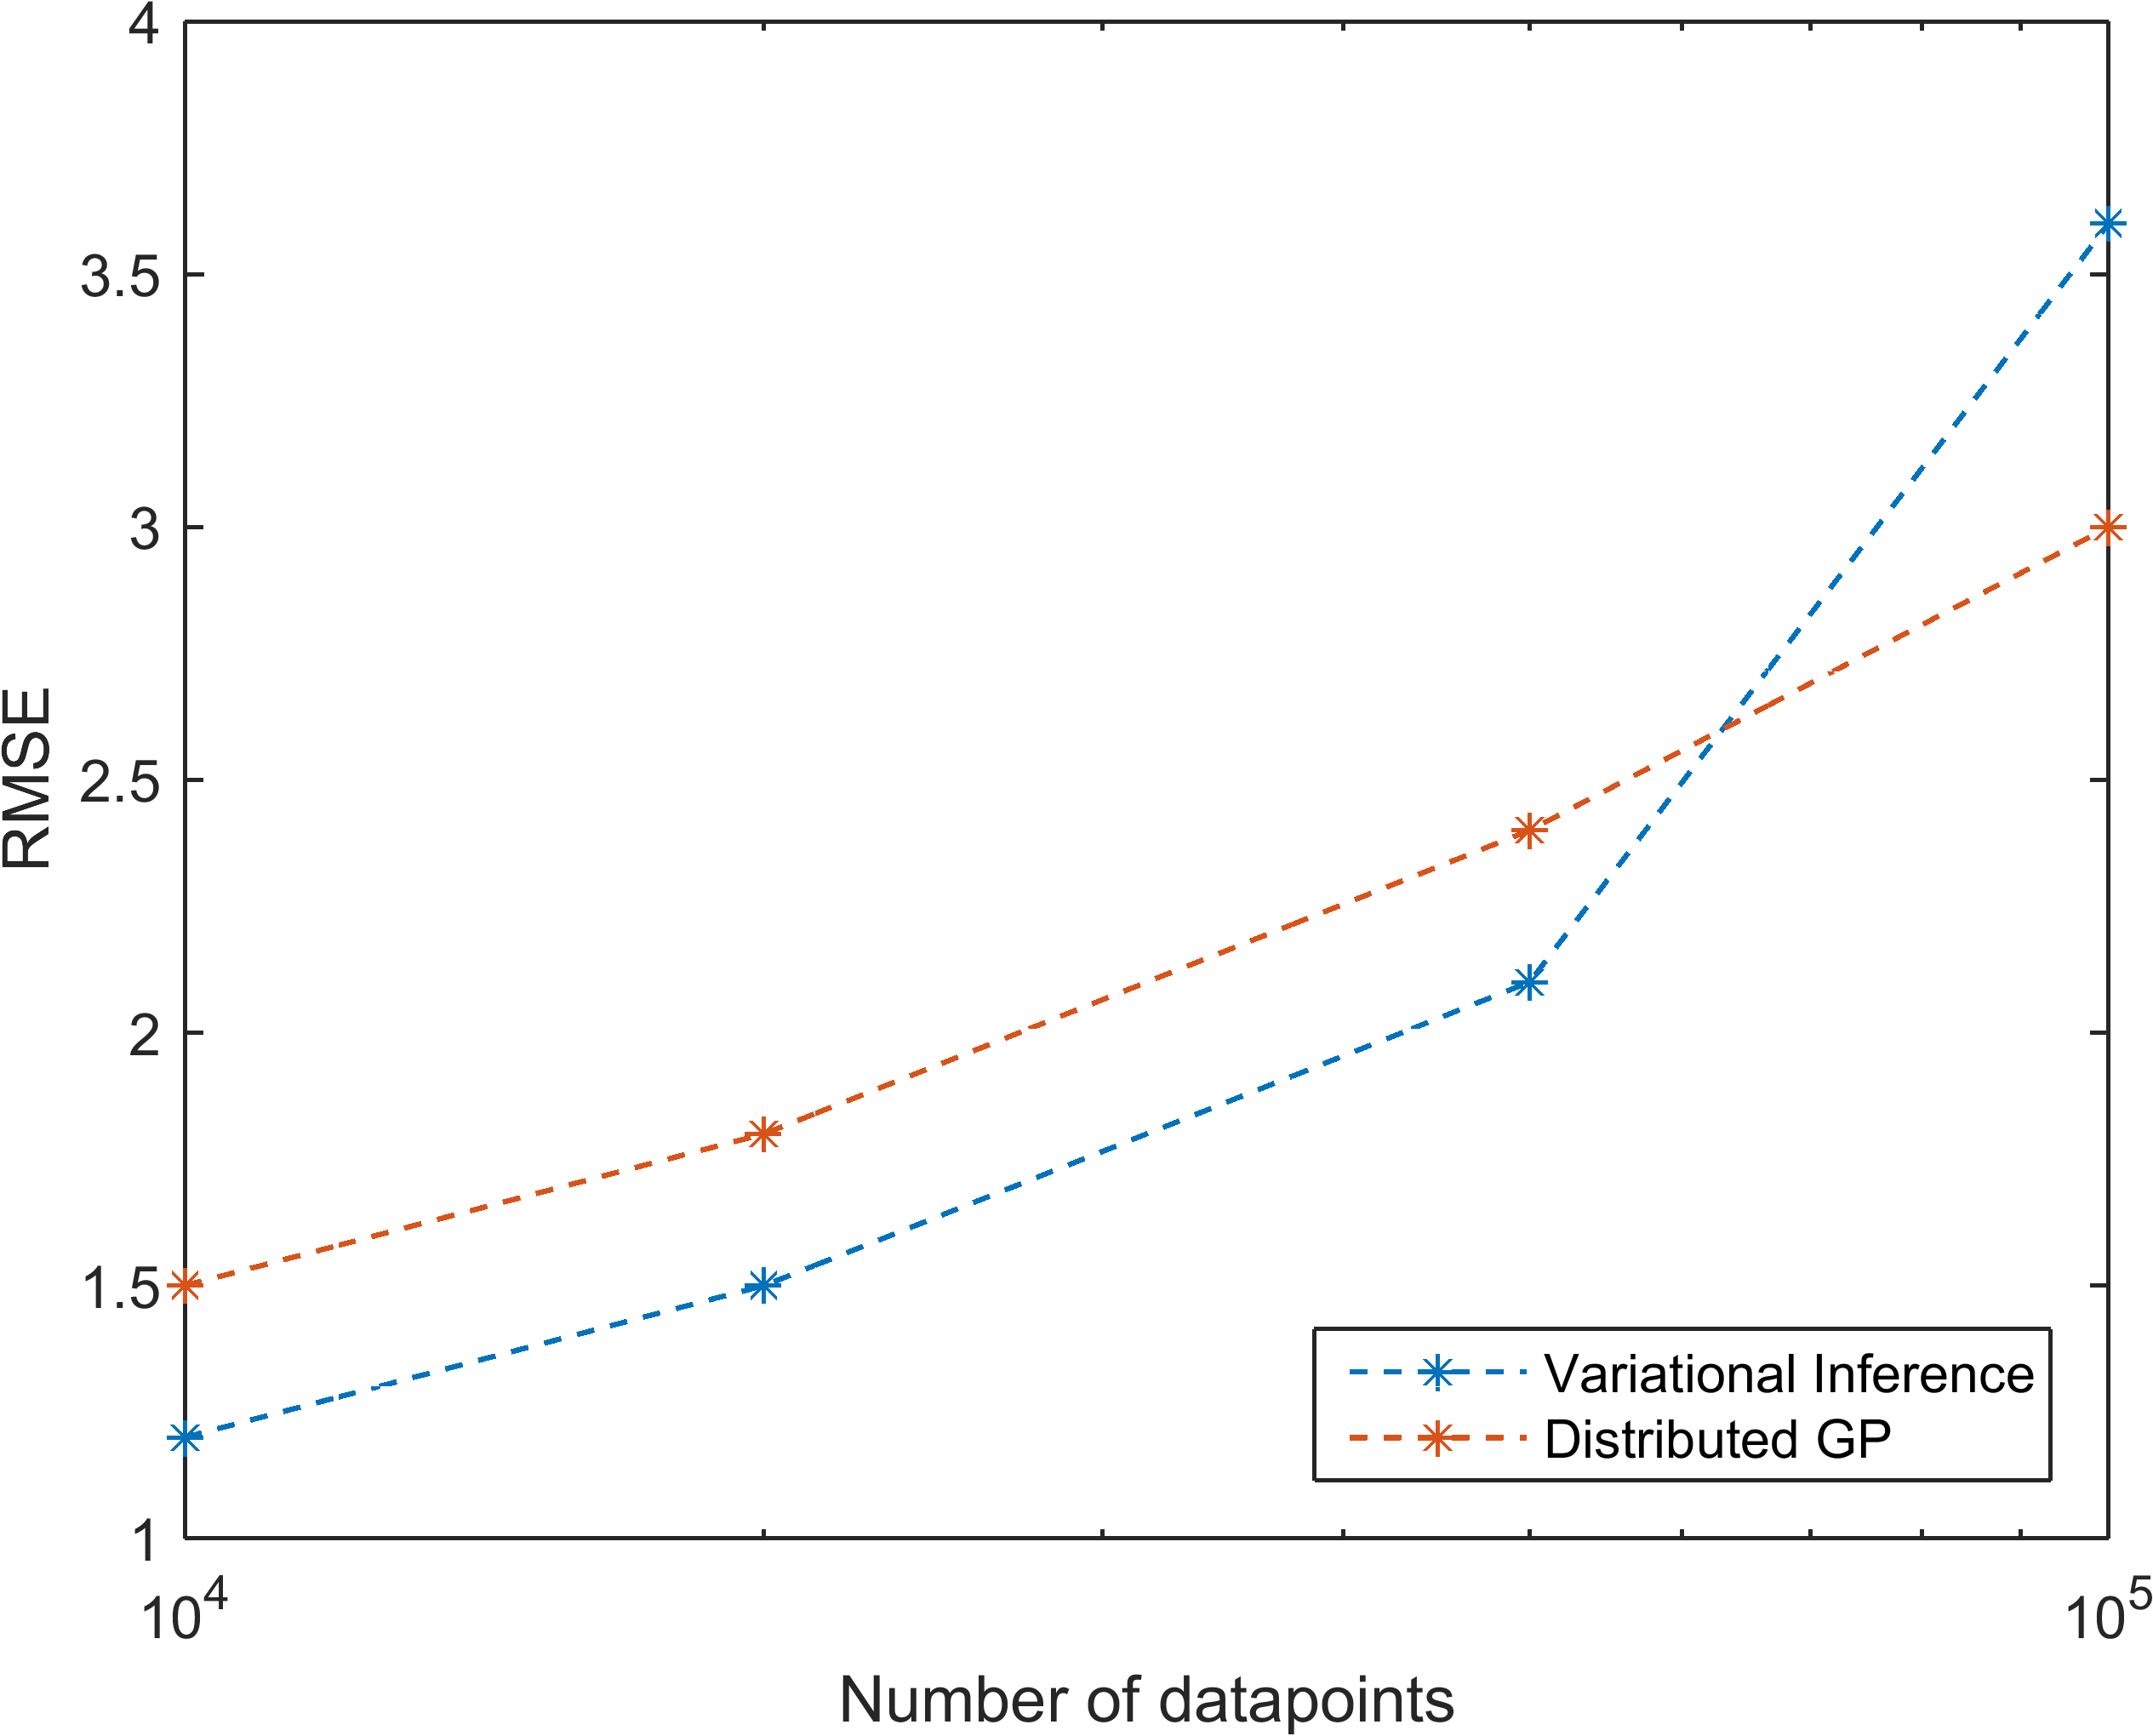
\includegraphics[width=0.48\textwidth]{images/comparisonOfRMSE}\label{subfig:comparisonOfRMSE}}
  \caption{Comparison of run time and RMSE between distributed GP and Variational Inference}\label{fig:comparisonOfDGPvsVARGP}
\end{figure*}

For the second experiment we compare the Root Mean Squared Error (RMSE) and run-times of distributed GP and Variational Inference algorithms while performing approximate inference. We progressively generate from 10e3 to 10e5 data-points according to the equations \ref{eq:experimentalSET} and \ref{eq:derivativeEquation}. We separated 75\% of the data as training set and 25\% of the data as the test set, the training and test sets were chosen randomly. The variational inference relationship kernel as described in section \ref{sec:varMOGP} with 100 equidistant inducing points was used. We learn the optimal values of hyper-parameters for all the sets of training data. The distributed GP algorithm as described in section \ref{sec:dMOGP} was used with randomly chosen 512 points per expert. We learn the optimal values of hyper-parameters for all the sets of training data. The accuracy is plotted as RMSE values with respect to the test set. The runtime is defined as time taken to calculate negative log marginal likelihood equations \ref{eq:lowerBoundMultiVarNLML} and  \ref{eq:dGPNLML}. The RMSE values are calculated for only the dependent output \(y_{1}\) and then plotted in the figure \ref{subfig:comparisonOfRunTimes}. 

In figure \ref{subfig:comparisonOfRunTimes} the time to calculate negative log-marginal likelihood with increasing number of training points is calculated. As expected the full GP takes more time when compared to variational inference or distributed GP algorithms. The Variational inference algorithm has better run-time till 10e4 data-points after that distributed GP takes lesser time. 
In figure \ref{subfig:comparisonOfRMSE} the RMSE error with test set is compared between the variational inference and distributed GP algorithm. Here too the variational inference algorithm performs better lesser number of datapoints but distributed GP starts performing better when we reach more than 10e4 datapoints. 

One thing to note is that we have fixed the number and position of inducing points while performing this experiment. While a more optimized set of inducing points will have better results, for datasets of the order 10e5 distributed GP algorithm starts outperforming variational inference. Moreover, upon observing figure \ref{subfig:distributedFullKernelMatrix} we can say that the covariance matrix in a joint GP setting is not diagonal in nature and hence an approximation technique which can compensate between low-rank approximation and diagonal approximation should be investigated \cite{march2015askit}.

\subsection{Experiments on Flight Test Data}\label{subsec:expFlightLoadsData}
We perform experiments on flight loads data produced during flight test phase at Airbus. Loads are measured across the wing span using strain gauges. Shear load \(T_{z}\) and bending moment \(M_{x}\) as described in figure \ref{fig:wingLoadDiagram} are used as two outputs for this exercise. \(\eta\) or point of action of forces and angle of attack \(\alpha\) are the two inputs. The aircraft is in quasi-equillibrium in all conditions and there are no dynamic effects observed throughout this dataset. All data is normalized according to airbus policy.

\begin{figure}
\centering
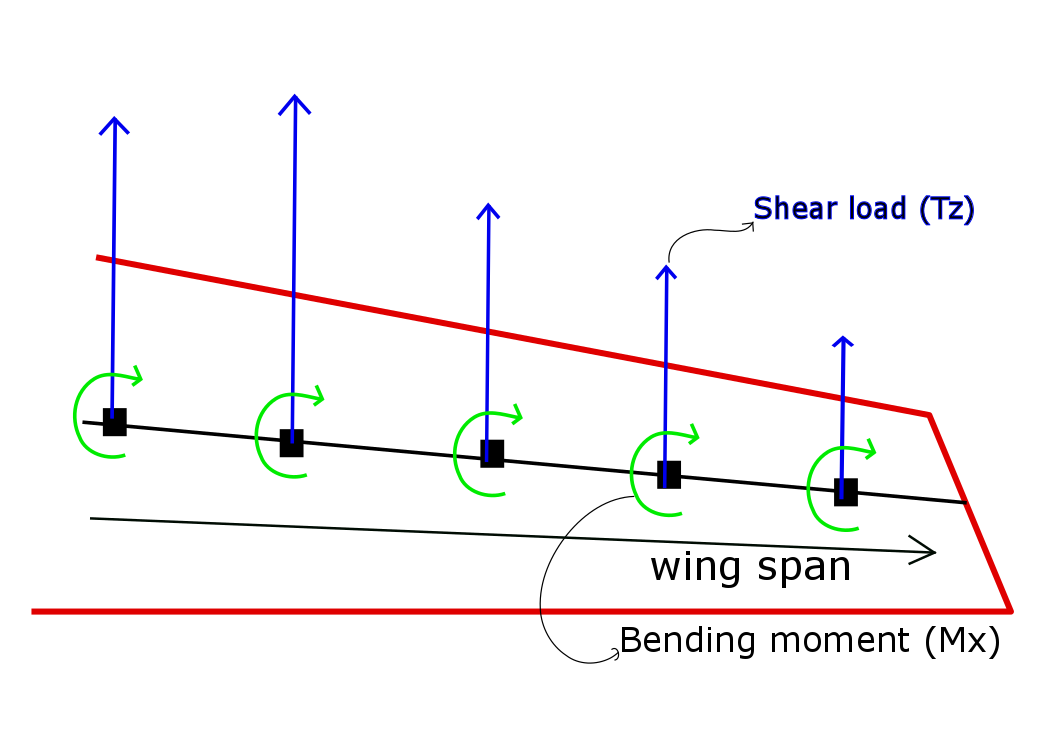
\includegraphics[width=0.5\columnwidth]{images/wingLoadDiagram.png}
\caption{Wing Load Diagram}
\label{fig:wingLoadDiagram}
\end{figure}


The relation between \(T_{z}\) and \(M_{x}\) can be written as:
\begin{equation}\label{eq:relationTzMx}
\centering
M_{x}(\eta, \alpha) = \int_{\eta}^{\eta_{edge}} T_{Z}(x, \alpha)(x-\eta)dx
\end{equation}.


The equation \ref{eq:relationTzMx} is applicable for the \(\eta\) axis. Here, \(\eta_{edge}\) denotes the edge of the wing span. The forces are measured at 5 points on the wing span and at 8800 points on the \(\alpha\) dimension. We compare plots of relationship-imposed multioutput GP and independent GP. Then we compare the measures of negative-log marginal likelihood and RMSE for varying number of inducing points.

\begin{figure*}[!t]
  \centering
  \subfigure[2\(\sigma\) confidence interval and mean of the dependent GP are represented in red shade and solid red line. 2\(\sigma\) confidence interval and mean of the independent GP are represented in blue shade and solid blue line. Experiment was run on 8800 data points Noisy data is denoted by circles only 1 \(\alpha\) step is plotted. Confidence interval improves upon adding the relationship kernel.]
  {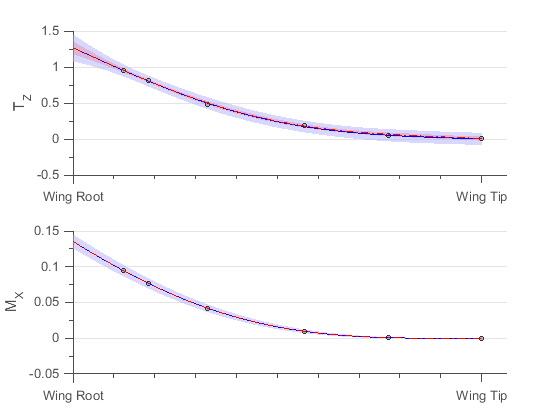
\includegraphics[width=0.48\textwidth]{images/experimental_plots.png}\label{subfig:experimental_plot}}\quad
  
  \subfigure[Progression of RMSE and log-likelihood upon increasing number of inducing points. Top plot shows the value of mean and variance of negative log-marginal likelihood. The bottom figure in blue shows the mean and variance of root mean squared error. 10 sets of experiments were run on 75\% of the data as training set and 25\% of the data as the test set, the training and test sets were chosen randomly.]
  {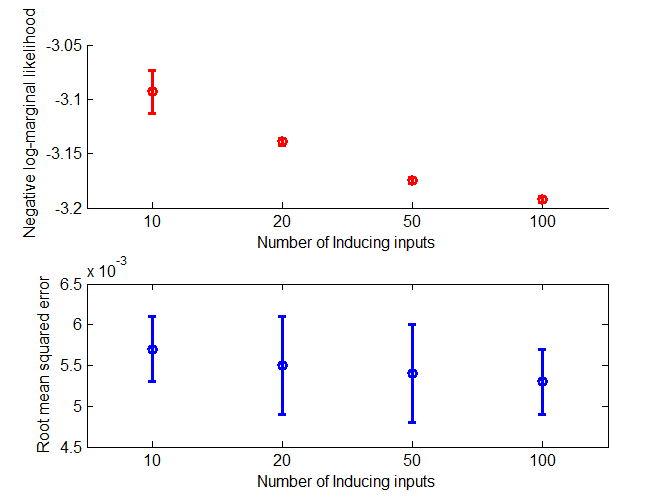
\includegraphics[width=0.48\textwidth]{images/experimental_output_nlml_error.png}\label{subfig:experimental_nlml_error}}
  \caption{Experimental results for aircraft flight loads}
\end{figure*}

Figure \ref{subfig:experimental_plot} shows the independent (blue shade) and joint fit (red shade) of two GP. The top figure shows \(T_{Z}\) with the variance of dependent GP plotted in red and variance of independent GP plotted in blue. Bottom figure shows plots for \(M_{X}\). Since the number of input points is less than 10e5 we use variational inference. 100 inducing points in the input space are used to learn and plot the figure. The variance of red is smaller than that of blue showing the improvement in confidence when imposing relationships in the GP architecture. The relationship between \(T_{Z}\) and \(M_{X}\) gives rise to better confidence during the loads prediction. This added information is very useful when identifying faulty sensor data since equation \ref{eq:relationTzMx} will push data points which do not satisfy the relationship out of the tight confidence interval.

Figure \ref{subfig:experimental_nlml_error} shows improvement in the negative log-marginal likelihood and RMSE plots upon increasing number of inducing points. 10 sets of experiments were run on 75\% of the data as training set and 25\% of the data as the test set, the training and test sets were chosen randomly. We learn the optimal values of hyper-parameters and inducing points for all the 10 sets of experiments of training data. Finally, RMSE values are evaluated with respect to the test set and negative log-marginal likelihood are evaluated for each learned model. The RMSE and log-likelihood improve upon increasing the number of inducing points. 
   

%%% Local Variables: 
%%% mode: latex
%%% TeX-master: "isae-report-template"
%%% End: 

